\documentclass[twoside]{book}

% Packages required by doxygen
\usepackage{fixltx2e}
\usepackage{calc}
\usepackage{doxygen}
\usepackage[export]{adjustbox} % also loads graphicx
\usepackage{graphicx}
\usepackage[utf8]{inputenc}
\usepackage{makeidx}
\usepackage{multicol}
\usepackage{multirow}
\PassOptionsToPackage{warn}{textcomp}
\usepackage{textcomp}
\usepackage[nointegrals]{wasysym}
\usepackage[table]{xcolor}

% Font selection
\usepackage[T1]{fontenc}
\usepackage[scaled=.90]{helvet}
\usepackage{courier}
\usepackage{amssymb}
\usepackage{sectsty}
\renewcommand{\familydefault}{\sfdefault}
\allsectionsfont{%
  \fontseries{bc}\selectfont%
  \color{darkgray}%
}
\renewcommand{\DoxyLabelFont}{%
  \fontseries{bc}\selectfont%
  \color{darkgray}%
}
\newcommand{\+}{\discretionary{\mbox{\scriptsize$\hookleftarrow$}}{}{}}

% Page & text layout
\usepackage{geometry}
\geometry{%
  a4paper,%
  top=2.5cm,%
  bottom=2.5cm,%
  left=2.5cm,%
  right=2.5cm%
}
\tolerance=750
\hfuzz=15pt
\hbadness=750
\setlength{\emergencystretch}{15pt}
\setlength{\parindent}{0cm}
\setlength{\parskip}{3ex plus 2ex minus 2ex}
\makeatletter
\renewcommand{\paragraph}{%
  \@startsection{paragraph}{4}{0ex}{-1.0ex}{1.0ex}{%
    \normalfont\normalsize\bfseries\SS@parafont%
  }%
}
\renewcommand{\subparagraph}{%
  \@startsection{subparagraph}{5}{0ex}{-1.0ex}{1.0ex}{%
    \normalfont\normalsize\bfseries\SS@subparafont%
  }%
}
\makeatother

% Headers & footers
\usepackage{fancyhdr}
\pagestyle{fancyplain}
\fancyhead[LE]{\fancyplain{}{\bfseries\thepage}}
\fancyhead[CE]{\fancyplain{}{}}
\fancyhead[RE]{\fancyplain{}{\bfseries\leftmark}}
\fancyhead[LO]{\fancyplain{}{\bfseries\rightmark}}
\fancyhead[CO]{\fancyplain{}{}}
\fancyhead[RO]{\fancyplain{}{\bfseries\thepage}}
\fancyfoot[LE]{\fancyplain{}{}}
\fancyfoot[CE]{\fancyplain{}{}}
\fancyfoot[RE]{\fancyplain{}{\bfseries\scriptsize Generated by Doxygen }}
\fancyfoot[LO]{\fancyplain{}{\bfseries\scriptsize Generated by Doxygen }}
\fancyfoot[CO]{\fancyplain{}{}}
\fancyfoot[RO]{\fancyplain{}{}}
\renewcommand{\footrulewidth}{0.4pt}
\renewcommand{\chaptermark}[1]{%
  \markboth{#1}{}%
}
\renewcommand{\sectionmark}[1]{%
  \markright{\thesection\ #1}%
}

% Indices & bibliography
\usepackage{natbib}
\usepackage[titles]{tocloft}
\setcounter{tocdepth}{3}
\setcounter{secnumdepth}{5}
\makeindex

% Hyperlinks (required, but should be loaded last)
\usepackage{ifpdf}
\ifpdf
  \usepackage[pdftex,pagebackref=true]{hyperref}
\else
  \usepackage[ps2pdf,pagebackref=true]{hyperref}
\fi
\hypersetup{%
  colorlinks=true,%
  linkcolor=blue,%
  citecolor=blue,%
  unicode%
}

% Custom commands
\newcommand{\clearemptydoublepage}{%
  \newpage{\pagestyle{empty}\cleardoublepage}%
}

\usepackage{caption}
\captionsetup{labelsep=space,justification=centering,font={bf},singlelinecheck=off,skip=4pt,position=top}

%===== C O N T E N T S =====

\begin{document}

% Titlepage & ToC
\hypersetup{pageanchor=false,
             bookmarksnumbered=true,
             pdfencoding=unicode
            }
\pagenumbering{alph}
\begin{titlepage}
\vspace*{7cm}
\begin{center}%
{\Large B\+K\+Engine \\[1ex]\large v1.\+3 }\\
\vspace*{1cm}
{\large Generated by Doxygen 1.8.13}\\
\end{center}
\end{titlepage}
\clearemptydoublepage
\pagenumbering{roman}
\tableofcontents
\clearemptydoublepage
\pagenumbering{arabic}
\hypersetup{pageanchor=true}

%--- Begin generated contents ---
\chapter{Hierarchical Index}
\section{Class Hierarchy}
This inheritance list is sorted roughly, but not completely, alphabetically\+:\begin{DoxyCompactList}
\item \contentsline{section}{bkengine\+:\+:Button}{\pageref{classbkengine_1_1Button}}{}
\item \contentsline{section}{bkengine\+:\+:Buttons}{\pageref{classbkengine_1_1Buttons}}{}
\item \contentsline{section}{bkengine\+:\+:Color}{\pageref{structbkengine_1_1Color}}{}
\item \contentsline{section}{bkengine\+:\+:Core}{\pageref{classbkengine_1_1Core}}{}
\item \contentsline{section}{bkengine\+:\+:Event}{\pageref{classbkengine_1_1Event}}{}
\item \contentsline{section}{bkengine\+:\+:Event\+Interface}{\pageref{classbkengine_1_1EventInterface}}{}
\begin{DoxyCompactList}
\item \contentsline{section}{bkengine\+:\+:S\+D\+L\+Event\+Interface}{\pageref{classbkengine_1_1SDLEventInterface}}{}
\end{DoxyCompactList}
\item \contentsline{section}{bkengine\+:\+:Fonts}{\pageref{classbkengine_1_1Fonts}}{}
\item \contentsline{section}{bkengine\+:\+:Game\+Serializer}{\pageref{classbkengine_1_1GameSerializer}}{}
\item \contentsline{section}{bkengine\+:\+:Key}{\pageref{classbkengine_1_1Key}}{}
\item \contentsline{section}{bkengine\+:\+:Keyboard\+Event}{\pageref{structbkengine_1_1KeyboardEvent}}{}
\item \contentsline{section}{bkengine\+:\+:Keys}{\pageref{classbkengine_1_1Keys}}{}
\item \contentsline{section}{bkengine\+:\+:Location}{\pageref{structbkengine_1_1Location}}{}
\item \contentsline{section}{bkengine\+:\+:Logger}{\pageref{classbkengine_1_1Logger}}{}
\item \contentsline{section}{bkengine\+:\+:Motion\+Event}{\pageref{structbkengine_1_1MotionEvent}}{}
\item \contentsline{section}{bkengine\+:\+:Mouse\+Event}{\pageref{structbkengine_1_1MouseEvent}}{}
\item \contentsline{section}{bkengine\+:\+:Rect}{\pageref{structbkengine_1_1Rect}}{}
\item \contentsline{section}{bkengine\+:\+:Relative\+Coordinates}{\pageref{classbkengine_1_1RelativeCoordinates}}{}
\item S\+DL\begin{DoxyCompactList}
\item \contentsline{section}{S\+D\+L\+Mock}{\pageref{classSDLMock}}{}
\end{DoxyCompactList}
\item \contentsline{section}{bkengine\+:\+:Serializable}{\pageref{classbkengine_1_1Serializable}}{}
\begin{DoxyCompactList}
\item \contentsline{section}{bkengine\+:\+:Animation}{\pageref{classbkengine_1_1Animation}}{}
\item \contentsline{section}{bkengine\+:\+:Element}{\pageref{classbkengine_1_1Element}}{}
\begin{DoxyCompactList}
\item \contentsline{section}{bkengine\+:\+:Entity}{\pageref{classbkengine_1_1Entity}}{}
\end{DoxyCompactList}
\item \contentsline{section}{bkengine\+:\+:Game}{\pageref{classbkengine_1_1Game}}{}
\item \contentsline{section}{bkengine\+:\+:Scene}{\pageref{classbkengine_1_1Scene}}{}
\item \contentsline{section}{bkengine\+:\+:Texture}{\pageref{classbkengine_1_1Texture}}{}
\begin{DoxyCompactList}
\item \contentsline{section}{Texture\+Mock}{\pageref{classTextureMock}}{}
\end{DoxyCompactList}
\end{DoxyCompactList}
\item \contentsline{section}{bkengine\+:\+:Serializer}{\pageref{classbkengine_1_1Serializer}}{}
\item \contentsline{section}{bkengine\+:\+:Settings\+Interface}{\pageref{classbkengine_1_1SettingsInterface}}{}
\begin{DoxyCompactList}
\item \contentsline{section}{bkengine\+:\+:I\+N\+I\+Settings\+Interface}{\pageref{classbkengine_1_1INISettingsInterface}}{}
\end{DoxyCompactList}
\item \contentsline{section}{bkengine\+:\+:Size}{\pageref{structbkengine_1_1Size}}{}
\item \contentsline{section}{bkengine\+:\+:Storage}{\pageref{classbkengine_1_1Storage}}{}
\item Test\begin{DoxyCompactList}
\item \contentsline{section}{Core\+Test}{\pageref{classCoreTest}}{}
\item \contentsline{section}{Texture\+Test}{\pageref{classTextureTest}}{}
\end{DoxyCompactList}
\item \contentsline{section}{bkengine\+:\+:Texture\+Wrapper}{\pageref{classbkengine_1_1TextureWrapper}}{}
\item \contentsline{section}{bkengine\+:\+:Timer}{\pageref{classbkengine_1_1Timer}}{}
\item \contentsline{section}{bkengine\+:\+:Wheel\+Event}{\pageref{structbkengine_1_1WheelEvent}}{}
\item \contentsline{section}{bkengine\+:\+:Window\+Event}{\pageref{structbkengine_1_1WindowEvent}}{}
\end{DoxyCompactList}

\chapter{Class Index}
\section{Class List}
Here are the classes, structs, unions and interfaces with brief descriptions\+:\begin{DoxyCompactList}
\item\contentsline{section}{\hyperlink{classbkengine_1_1Animation}{bkengine\+::\+Animation} }{\pageref{classbkengine_1_1Animation}}{}
\item\contentsline{section}{\hyperlink{classbkengine_1_1Button}{bkengine\+::\+Button} }{\pageref{classbkengine_1_1Button}}{}
\item\contentsline{section}{\hyperlink{classbkengine_1_1Buttons}{bkengine\+::\+Buttons} }{\pageref{classbkengine_1_1Buttons}}{}
\item\contentsline{section}{\hyperlink{structbkengine_1_1Color}{bkengine\+::\+Color} }{\pageref{structbkengine_1_1Color}}{}
\item\contentsline{section}{\hyperlink{classbkengine_1_1Core}{bkengine\+::\+Core} }{\pageref{classbkengine_1_1Core}}{}
\item\contentsline{section}{\hyperlink{classCoreTest}{Core\+Test} }{\pageref{classCoreTest}}{}
\item\contentsline{section}{\hyperlink{classbkengine_1_1Element}{bkengine\+::\+Element} }{\pageref{classbkengine_1_1Element}}{}
\item\contentsline{section}{\hyperlink{classbkengine_1_1Entity}{bkengine\+::\+Entity} }{\pageref{classbkengine_1_1Entity}}{}
\item\contentsline{section}{\hyperlink{classbkengine_1_1Event}{bkengine\+::\+Event} }{\pageref{classbkengine_1_1Event}}{}
\item\contentsline{section}{\hyperlink{classbkengine_1_1EventInterface}{bkengine\+::\+Event\+Interface} }{\pageref{classbkengine_1_1EventInterface}}{}
\item\contentsline{section}{\hyperlink{classbkengine_1_1Fonts}{bkengine\+::\+Fonts} }{\pageref{classbkengine_1_1Fonts}}{}
\item\contentsline{section}{\hyperlink{classbkengine_1_1Game}{bkengine\+::\+Game} }{\pageref{classbkengine_1_1Game}}{}
\item\contentsline{section}{\hyperlink{classbkengine_1_1GameSerializer}{bkengine\+::\+Game\+Serializer} }{\pageref{classbkengine_1_1GameSerializer}}{}
\item\contentsline{section}{\hyperlink{classbkengine_1_1INISettingsInterface}{bkengine\+::\+I\+N\+I\+Settings\+Interface} }{\pageref{classbkengine_1_1INISettingsInterface}}{}
\item\contentsline{section}{\hyperlink{classbkengine_1_1Key}{bkengine\+::\+Key} }{\pageref{classbkengine_1_1Key}}{}
\item\contentsline{section}{\hyperlink{structbkengine_1_1KeyboardEvent}{bkengine\+::\+Keyboard\+Event} }{\pageref{structbkengine_1_1KeyboardEvent}}{}
\item\contentsline{section}{\hyperlink{classbkengine_1_1Keys}{bkengine\+::\+Keys} }{\pageref{classbkengine_1_1Keys}}{}
\item\contentsline{section}{\hyperlink{structbkengine_1_1Location}{bkengine\+::\+Location} }{\pageref{structbkengine_1_1Location}}{}
\item\contentsline{section}{\hyperlink{classbkengine_1_1Logger}{bkengine\+::\+Logger} }{\pageref{classbkengine_1_1Logger}}{}
\item\contentsline{section}{\hyperlink{structbkengine_1_1MotionEvent}{bkengine\+::\+Motion\+Event} }{\pageref{structbkengine_1_1MotionEvent}}{}
\item\contentsline{section}{\hyperlink{structbkengine_1_1MouseEvent}{bkengine\+::\+Mouse\+Event} }{\pageref{structbkengine_1_1MouseEvent}}{}
\item\contentsline{section}{\hyperlink{structbkengine_1_1Rect}{bkengine\+::\+Rect} }{\pageref{structbkengine_1_1Rect}}{}
\item\contentsline{section}{\hyperlink{classbkengine_1_1RelativeCoordinates}{bkengine\+::\+Relative\+Coordinates} }{\pageref{classbkengine_1_1RelativeCoordinates}}{}
\item\contentsline{section}{\hyperlink{classbkengine_1_1Scene}{bkengine\+::\+Scene} }{\pageref{classbkengine_1_1Scene}}{}
\item\contentsline{section}{\hyperlink{classbkengine_1_1SDLEventInterface}{bkengine\+::\+S\+D\+L\+Event\+Interface} }{\pageref{classbkengine_1_1SDLEventInterface}}{}
\item\contentsline{section}{\hyperlink{classSDLMock}{S\+D\+L\+Mock} }{\pageref{classSDLMock}}{}
\item\contentsline{section}{\hyperlink{classbkengine_1_1Serializable}{bkengine\+::\+Serializable} }{\pageref{classbkengine_1_1Serializable}}{}
\item\contentsline{section}{\hyperlink{classbkengine_1_1Serializer}{bkengine\+::\+Serializer} }{\pageref{classbkengine_1_1Serializer}}{}
\item\contentsline{section}{\hyperlink{classbkengine_1_1SettingsInterface}{bkengine\+::\+Settings\+Interface} }{\pageref{classbkengine_1_1SettingsInterface}}{}
\item\contentsline{section}{\hyperlink{structbkengine_1_1Size}{bkengine\+::\+Size} }{\pageref{structbkengine_1_1Size}}{}
\item\contentsline{section}{\hyperlink{classbkengine_1_1Storage}{bkengine\+::\+Storage} }{\pageref{classbkengine_1_1Storage}}{}
\item\contentsline{section}{\hyperlink{classbkengine_1_1Texture}{bkengine\+::\+Texture} }{\pageref{classbkengine_1_1Texture}}{}
\item\contentsline{section}{\hyperlink{classTextureMock}{Texture\+Mock} }{\pageref{classTextureMock}}{}
\item\contentsline{section}{\hyperlink{classTextureTest}{Texture\+Test} }{\pageref{classTextureTest}}{}
\item\contentsline{section}{\hyperlink{classbkengine_1_1TextureWrapper}{bkengine\+::\+Texture\+Wrapper} }{\pageref{classbkengine_1_1TextureWrapper}}{}
\item\contentsline{section}{\hyperlink{classbkengine_1_1Timer}{bkengine\+::\+Timer} }{\pageref{classbkengine_1_1Timer}}{}
\item\contentsline{section}{\hyperlink{structbkengine_1_1WheelEvent}{bkengine\+::\+Wheel\+Event} }{\pageref{structbkengine_1_1WheelEvent}}{}
\item\contentsline{section}{\hyperlink{structbkengine_1_1WindowEvent}{bkengine\+::\+Window\+Event} }{\pageref{structbkengine_1_1WindowEvent}}{}
\end{DoxyCompactList}

\chapter{Class Documentation}
\hypertarget{classbkengine_1_1Animation}{}\section{bkengine\+:\+:Animation Class Reference}
\label{classbkengine_1_1Animation}\index{bkengine\+::\+Animation@{bkengine\+::\+Animation}}
Inheritance diagram for bkengine\+:\+:Animation\+:\begin{figure}[H]
\begin{center}
\leavevmode
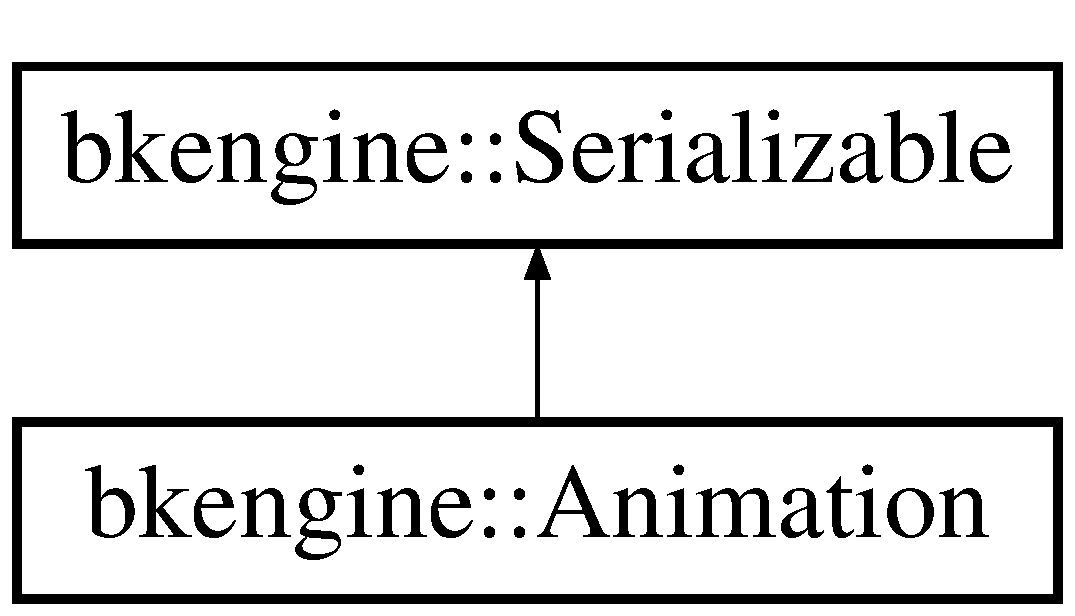
\includegraphics[height=2.000000cm]{classbkengine_1_1Animation}
\end{center}
\end{figure}
\subsection*{Public Member Functions}
\begin{DoxyCompactItemize}
\item 
\mbox{\Hypertarget{classbkengine_1_1Animation_af822f84e07cf2258dbaa85875c08f875}\label{classbkengine_1_1Animation_af822f84e07cf2258dbaa85875c08f875}} 
{\footnotesize template$<$typename T $>$ }\\void {\bfseries add\+Image} (const std\+::string \&path, const \hyperlink{structbkengine_1_1Rect}{Rect} \&clip=\hyperlink{structbkengine_1_1Rect}{Rect}(), const \hyperlink{structbkengine_1_1Rect}{Rect} \&size=\hyperlink{structbkengine_1_1Rect}{Rect}())
\item 
\mbox{\Hypertarget{classbkengine_1_1Animation_a856a210f9d966d910287690a6dbecb23}\label{classbkengine_1_1Animation_a856a210f9d966d910287690a6dbecb23}} 
{\footnotesize template$<$typename T $>$ }\\void {\bfseries add\+Text} (const std\+::string \&font\+Name, const std\+::string \&text, const \hyperlink{structbkengine_1_1Rect}{Rect} \&size, const \hyperlink{structbkengine_1_1Color}{Color} \&color=\hyperlink{structbkengine_1_1Color}{Color}(), Text\+Quality quality=Text\+Quality\+::\+S\+O\+L\+ID)
\item 
\mbox{\Hypertarget{classbkengine_1_1Animation_a1f322fcb75e0128ae9a61580291c5637}\label{classbkengine_1_1Animation_a1f322fcb75e0128ae9a61580291c5637}} 
{\footnotesize template$<$typename T $>$ }\\void {\bfseries add\+Texture} (const T \&texture)
\item 
\mbox{\Hypertarget{classbkengine_1_1Animation_a44c346878aafe731e46f303d518affe0}\label{classbkengine_1_1Animation_a44c346878aafe731e46f303d518affe0}} 
{\footnotesize template$<$typename T $>$ }\\void {\bfseries add\+Texture} (std\+::shared\+\_\+ptr$<$ T $>$ texture)
\item 
\mbox{\Hypertarget{classbkengine_1_1Animation_a41a3d19e22693a3cf8d82309d6ef9580}\label{classbkengine_1_1Animation_a41a3d19e22693a3cf8d82309d6ef9580}} 
bool {\bfseries has\+Texture} (unsigned int index) const
\item 
\mbox{\Hypertarget{classbkengine_1_1Animation_a949c440102e5e9c419829992d7902df8}\label{classbkengine_1_1Animation_a949c440102e5e9c419829992d7902df8}} 
\hyperlink{classbkengine_1_1Texture}{Texture} \& {\bfseries get\+Next\+Texture} ()
\item 
\mbox{\Hypertarget{classbkengine_1_1Animation_a89e013f462bfe414f152e256ea810ca8}\label{classbkengine_1_1Animation_a89e013f462bfe414f152e256ea810ca8}} 
\hyperlink{classbkengine_1_1Texture}{Texture} \& {\bfseries get\+Current\+Texture} ()
\item 
\mbox{\Hypertarget{classbkengine_1_1Animation_a88b2acdb20e401e8552556564c12616b}\label{classbkengine_1_1Animation_a88b2acdb20e401e8552556564c12616b}} 
std\+::string {\bfseries get\+Name} () const
\item 
\mbox{\Hypertarget{classbkengine_1_1Animation_a822b375e03043c1e4304b052caadac2f}\label{classbkengine_1_1Animation_a822b375e03043c1e4304b052caadac2f}} 
{\bfseries Animation} (const std\+::string \&descr=\char`\"{}\char`\"{}, unsigned int frame\+Delta=1)
\item 
\mbox{\Hypertarget{classbkengine_1_1Animation_a512e289acbec4df552208d155412e4e1}\label{classbkengine_1_1Animation_a512e289acbec4df552208d155412e4e1}} 
void {\bfseries inc\+Frame\+Count} ()
\item 
\mbox{\Hypertarget{classbkengine_1_1Animation_ae70c8cb0878bf32a2486b69d34ee0fa7}\label{classbkengine_1_1Animation_ae70c8cb0878bf32a2486b69d34ee0fa7}} 
void {\bfseries set\+Frames\+Per\+Texture} (unsigned int frames)
\item 
\mbox{\Hypertarget{classbkengine_1_1Animation_a903eb4b61b8c7bc72bbedbdba4cbb501}\label{classbkengine_1_1Animation_a903eb4b61b8c7bc72bbedbdba4cbb501}} 
void {\bfseries reset} ()
\item 
\mbox{\Hypertarget{classbkengine_1_1Animation_ac55679938c88e9477e298973bcb43022}\label{classbkengine_1_1Animation_ac55679938c88e9477e298973bcb43022}} 
virtual void {\bfseries setup\+Textures} ()
\item 
\mbox{\Hypertarget{classbkengine_1_1Animation_a06d0f816e562efcc53a52db8463a683a}\label{classbkengine_1_1Animation_a06d0f816e562efcc53a52db8463a683a}} 
virtual void {\bfseries setup\+Environment} ()
\item 
\mbox{\Hypertarget{classbkengine_1_1Animation_a53f49f65aad3c3c442a8212862400c84}\label{classbkengine_1_1Animation_a53f49f65aad3c3c442a8212862400c84}} 
virtual void {\bfseries deserialize} (const Json\+::\+Value \&) override
\item 
\mbox{\Hypertarget{classbkengine_1_1Animation_a089b67a89dbf3529cbcc48a7ea84dd85}\label{classbkengine_1_1Animation_a089b67a89dbf3529cbcc48a7ea84dd85}} 
virtual Json\+::\+Value {\bfseries serialize} () const override
\item 
\mbox{\Hypertarget{classbkengine_1_1Animation_a99fce2e0d0de7f16c3015c59447956cb}\label{classbkengine_1_1Animation_a99fce2e0d0de7f16c3015c59447956cb}} 
{\footnotesize template$<$typename T $>$ }\\void {\bfseries add\+Image} (const std\+::string \&path, const \hyperlink{structbkengine_1_1Rect}{Rect} \&size, const \hyperlink{structbkengine_1_1Rect}{Rect} \&clip)
\item 
\mbox{\Hypertarget{classbkengine_1_1Animation_a96db630ab68419582cae430efb7cf0ed}\label{classbkengine_1_1Animation_a96db630ab68419582cae430efb7cf0ed}} 
{\footnotesize template$<$typename T $>$ }\\void {\bfseries add\+Text} (const std\+::string \&font\+Name, const std\+::string \&text, const \hyperlink{structbkengine_1_1Rect}{Rect} \&size, const \hyperlink{structbkengine_1_1Color}{Color} \&color, Text\+Quality quality)
\item 
\mbox{\Hypertarget{classbkengine_1_1Animation_a1f322fcb75e0128ae9a61580291c5637}\label{classbkengine_1_1Animation_a1f322fcb75e0128ae9a61580291c5637}} 
{\footnotesize template$<$typename T $>$ }\\void {\bfseries add\+Texture} (const T \&texture)
\item 
\mbox{\Hypertarget{classbkengine_1_1Animation_a44c346878aafe731e46f303d518affe0}\label{classbkengine_1_1Animation_a44c346878aafe731e46f303d518affe0}} 
{\footnotesize template$<$typename T $>$ }\\void {\bfseries add\+Texture} (std\+::shared\+\_\+ptr$<$ T $>$ texture)
\end{DoxyCompactItemize}


\subsection{Detailed Description}


Definition at line 16 of file Animation.\+h.



The documentation for this class was generated from the following files\+:\begin{DoxyCompactItemize}
\item 
/home/skaupper/dev/\+B\+K\+Engine/include/bkengine/Animation.\+h\item 
/home/skaupper/dev/\+B\+K\+Engine/include/bkengine/templates/Animation\+\_\+templates.\+h\item 
/home/skaupper/dev/\+B\+K\+Engine/src/Animation.\+cpp\end{DoxyCompactItemize}

\hypertarget{classbkengine_1_1Button}{}\section{bkengine\+:\+:Button Class Reference}
\label{classbkengine_1_1Button}\index{bkengine\+::\+Button@{bkengine\+::\+Button}}
\subsection*{Public Member Functions}
\begin{DoxyCompactItemize}
\item 
\mbox{\Hypertarget{classbkengine_1_1Button_a07d94c1cf55fc36edd123b02217af399}\label{classbkengine_1_1Button_a07d94c1cf55fc36edd123b02217af399}} 
{\bfseries Button} (const std\+::string \&button\+String)
\item 
\mbox{\Hypertarget{classbkengine_1_1Button_ac7c2bc4c54d0cc9fefd082c9d6c575dd}\label{classbkengine_1_1Button_ac7c2bc4c54d0cc9fefd082c9d6c575dd}} 
bool {\bfseries operator==} (const \hyperlink{classbkengine_1_1Button}{Button} \&) const
\item 
\mbox{\Hypertarget{classbkengine_1_1Button_a9436026b1ecd0705629ef795ce43e345}\label{classbkengine_1_1Button_a9436026b1ecd0705629ef795ce43e345}} 
bool {\bfseries operator!=} (const \hyperlink{classbkengine_1_1Button}{Button} \&) const
\item 
\mbox{\Hypertarget{classbkengine_1_1Button_a77b7b58ddc9879eb051d0e3de651a2bb}\label{classbkengine_1_1Button_a77b7b58ddc9879eb051d0e3de651a2bb}} 
{\bfseries operator const std\+::string} () const
\item 
\mbox{\Hypertarget{classbkengine_1_1Button_af83d858e8e6f0f7fe868a65ac7a08fa6}\label{classbkengine_1_1Button_af83d858e8e6f0f7fe868a65ac7a08fa6}} 
std\+::string {\bfseries to\+String} ()
\end{DoxyCompactItemize}


\subsection{Detailed Description}


Definition at line 169 of file Keys.\+h.



The documentation for this class was generated from the following files\+:\begin{DoxyCompactItemize}
\item 
/home/skaupper/dev/\+B\+K\+Engine/include/bkengine/Keys.\+h\item 
/home/skaupper/dev/\+B\+K\+Engine/src/Keys.\+cpp\end{DoxyCompactItemize}

\hypertarget{classbkengine_1_1Buttons}{}\section{bkengine\+:\+:Buttons Class Reference}
\label{classbkengine_1_1Buttons}\index{bkengine\+::\+Buttons@{bkengine\+::\+Buttons}}
\subsection*{Static Public Attributes}
\begin{DoxyCompactItemize}
\item 
\mbox{\Hypertarget{classbkengine_1_1Buttons_ab1fddb89d67c630a0f7d617905ca7277}\label{classbkengine_1_1Buttons_ab1fddb89d67c630a0f7d617905ca7277}} 
static \hyperlink{classbkengine_1_1Button}{Button} {\bfseries U\+N\+K\+N\+O\+WN}
\item 
\mbox{\Hypertarget{classbkengine_1_1Buttons_a63338fac460ba72b47d48e31fb0a19fe}\label{classbkengine_1_1Buttons_a63338fac460ba72b47d48e31fb0a19fe}} 
static \hyperlink{classbkengine_1_1Button}{Button} {\bfseries L\+E\+FT}
\item 
\mbox{\Hypertarget{classbkengine_1_1Buttons_a4017a23786d5f14a2fe54ed6bde537c7}\label{classbkengine_1_1Buttons_a4017a23786d5f14a2fe54ed6bde537c7}} 
static \hyperlink{classbkengine_1_1Button}{Button} {\bfseries R\+I\+G\+HT}
\item 
\mbox{\Hypertarget{classbkengine_1_1Buttons_a753d46b26d0911ed56d9cb46ae7e385a}\label{classbkengine_1_1Buttons_a753d46b26d0911ed56d9cb46ae7e385a}} 
static \hyperlink{classbkengine_1_1Button}{Button} {\bfseries M\+I\+D\+D\+LE}
\item 
\mbox{\Hypertarget{classbkengine_1_1Buttons_a7d39cae81f36e23e27a270115f08e703}\label{classbkengine_1_1Buttons_a7d39cae81f36e23e27a270115f08e703}} 
static \hyperlink{classbkengine_1_1Button}{Button} {\bfseries S\+P\+E\+C\+I\+AL}
\end{DoxyCompactItemize}


\subsection{Detailed Description}


Definition at line 184 of file Keys.\+h.



The documentation for this class was generated from the following files\+:\begin{DoxyCompactItemize}
\item 
/home/skaupper/dev/\+B\+K\+Engine/include/bkengine/Keys.\+h\item 
/home/skaupper/dev/\+B\+K\+Engine/src/Keys.\+cpp\end{DoxyCompactItemize}

\hypertarget{structbkengine_1_1Color}{}\section{bkengine\+:\+:Color Struct Reference}
\label{structbkengine_1_1Color}\index{bkengine\+::\+Color@{bkengine\+::\+Color}}
\subsection*{Public Member Functions}
\begin{DoxyCompactItemize}
\item 
\mbox{\Hypertarget{structbkengine_1_1Color_a5dd1068a86959dfc7a25930148b24d08}\label{structbkengine_1_1Color_a5dd1068a86959dfc7a25930148b24d08}} 
{\bfseries Color} (uint8\+\_\+t r, uint8\+\_\+t g, uint8\+\_\+t b)
\item 
\mbox{\Hypertarget{structbkengine_1_1Color_ab8f3c9a331a6573972030dab578e20a2}\label{structbkengine_1_1Color_ab8f3c9a331a6573972030dab578e20a2}} 
{\bfseries Color} (uint8\+\_\+t r, uint8\+\_\+t g, uint8\+\_\+t b, uint8\+\_\+t a)
\item 
\mbox{\Hypertarget{structbkengine_1_1Color_abb8258c40a757066e26538b6c4be9ed0}\label{structbkengine_1_1Color_abb8258c40a757066e26538b6c4be9ed0}} 
std\+::string {\bfseries to\+String} () const
\item 
\mbox{\Hypertarget{structbkengine_1_1Color_ac87cb4e25b3c6f87fa7a713fc757114b}\label{structbkengine_1_1Color_ac87cb4e25b3c6f87fa7a713fc757114b}} 
bool {\bfseries operator==} (const \hyperlink{structbkengine_1_1Color}{Color} \&c) const
\item 
\mbox{\Hypertarget{structbkengine_1_1Color_acbf042e3979d8e6c6a62d7871d04303c}\label{structbkengine_1_1Color_acbf042e3979d8e6c6a62d7871d04303c}} 
bool {\bfseries operator$<$} (const \hyperlink{structbkengine_1_1Color}{Color} \&c) const
\end{DoxyCompactItemize}
\subsection*{Public Attributes}
\begin{DoxyCompactItemize}
\item 
\mbox{\Hypertarget{structbkengine_1_1Color_ae1a6df2184f20c5407a09dfbd4427b09}\label{structbkengine_1_1Color_ae1a6df2184f20c5407a09dfbd4427b09}} 
uint8\+\_\+t {\bfseries r}
\item 
\mbox{\Hypertarget{structbkengine_1_1Color_adf6701cc0f56d6c473237411ec1b5b2e}\label{structbkengine_1_1Color_adf6701cc0f56d6c473237411ec1b5b2e}} 
uint8\+\_\+t {\bfseries g}
\item 
\mbox{\Hypertarget{structbkengine_1_1Color_aafbce92f95824ea1cf56f1766c2480fb}\label{structbkengine_1_1Color_aafbce92f95824ea1cf56f1766c2480fb}} 
uint8\+\_\+t {\bfseries b}
\item 
\mbox{\Hypertarget{structbkengine_1_1Color_a062d260f16319d1865efe4151a58c109}\label{structbkengine_1_1Color_a062d260f16319d1865efe4151a58c109}} 
uint8\+\_\+t {\bfseries a}
\end{DoxyCompactItemize}
\subsection*{Static Public Attributes}
\begin{DoxyCompactItemize}
\item 
\mbox{\Hypertarget{structbkengine_1_1Color_a6f7dc225ef0b3dde655cbf925cad882d}\label{structbkengine_1_1Color_a6f7dc225ef0b3dde655cbf925cad882d}} 
static \hyperlink{structbkengine_1_1Color}{Color} {\bfseries B\+L\+A\+CK}
\item 
\mbox{\Hypertarget{structbkengine_1_1Color_aafb827ace5780d74f0c513ce92077853}\label{structbkengine_1_1Color_aafb827ace5780d74f0c513ce92077853}} 
static \hyperlink{structbkengine_1_1Color}{Color} {\bfseries W\+H\+I\+TE}
\item 
\mbox{\Hypertarget{structbkengine_1_1Color_abe0e77f1bd12cb0e98b4d5650009942c}\label{structbkengine_1_1Color_abe0e77f1bd12cb0e98b4d5650009942c}} 
static \hyperlink{structbkengine_1_1Color}{Color} {\bfseries R\+ED}
\item 
\mbox{\Hypertarget{structbkengine_1_1Color_a190dca9187728f879cd3487b24499baf}\label{structbkengine_1_1Color_a190dca9187728f879cd3487b24499baf}} 
static \hyperlink{structbkengine_1_1Color}{Color} {\bfseries L\+I\+ME}
\item 
\mbox{\Hypertarget{structbkengine_1_1Color_a5a1557101e389271fe14dceef583799a}\label{structbkengine_1_1Color_a5a1557101e389271fe14dceef583799a}} 
static \hyperlink{structbkengine_1_1Color}{Color} {\bfseries B\+L\+UE}
\item 
\mbox{\Hypertarget{structbkengine_1_1Color_ad7b2412aba74d8d4b5e6d6dc7627264d}\label{structbkengine_1_1Color_ad7b2412aba74d8d4b5e6d6dc7627264d}} 
static \hyperlink{structbkengine_1_1Color}{Color} {\bfseries Y\+E\+L\+L\+OW}
\item 
\mbox{\Hypertarget{structbkengine_1_1Color_aac281bf6e998aeef6f7e7c0c7df8dc34}\label{structbkengine_1_1Color_aac281bf6e998aeef6f7e7c0c7df8dc34}} 
static \hyperlink{structbkengine_1_1Color}{Color} {\bfseries C\+Y\+AN}
\item 
\mbox{\Hypertarget{structbkengine_1_1Color_a5db67dc17b725499d542d194cf1d475e}\label{structbkengine_1_1Color_a5db67dc17b725499d542d194cf1d475e}} 
static \hyperlink{structbkengine_1_1Color}{Color} {\bfseries M\+A\+G\+E\+N\+TA}
\item 
\mbox{\Hypertarget{structbkengine_1_1Color_a353855e6e05cd5ec048f658aa1906687}\label{structbkengine_1_1Color_a353855e6e05cd5ec048f658aa1906687}} 
static \hyperlink{structbkengine_1_1Color}{Color} {\bfseries S\+I\+L\+V\+ER}
\item 
\mbox{\Hypertarget{structbkengine_1_1Color_a6cba9bfb74c16863201155f01da97461}\label{structbkengine_1_1Color_a6cba9bfb74c16863201155f01da97461}} 
static \hyperlink{structbkengine_1_1Color}{Color} {\bfseries G\+R\+AY}
\item 
\mbox{\Hypertarget{structbkengine_1_1Color_a3f0f92edddf69f742cf4751e91276bcd}\label{structbkengine_1_1Color_a3f0f92edddf69f742cf4751e91276bcd}} 
static \hyperlink{structbkengine_1_1Color}{Color} {\bfseries M\+A\+R\+O\+ON}
\item 
\mbox{\Hypertarget{structbkengine_1_1Color_a84035523724f908034a9e3e893058bfb}\label{structbkengine_1_1Color_a84035523724f908034a9e3e893058bfb}} 
static \hyperlink{structbkengine_1_1Color}{Color} {\bfseries O\+L\+I\+VE}
\item 
\mbox{\Hypertarget{structbkengine_1_1Color_a5b9aafb544d41992e367b065e6595143}\label{structbkengine_1_1Color_a5b9aafb544d41992e367b065e6595143}} 
static \hyperlink{structbkengine_1_1Color}{Color} {\bfseries G\+R\+E\+EN}
\item 
\mbox{\Hypertarget{structbkengine_1_1Color_a130287f8f4e91c9c567ea0cc27f5f012}\label{structbkengine_1_1Color_a130287f8f4e91c9c567ea0cc27f5f012}} 
static \hyperlink{structbkengine_1_1Color}{Color} {\bfseries P\+U\+R\+P\+LE}
\item 
\mbox{\Hypertarget{structbkengine_1_1Color_a9853aa37a061c26fe3544489f2c93869}\label{structbkengine_1_1Color_a9853aa37a061c26fe3544489f2c93869}} 
static \hyperlink{structbkengine_1_1Color}{Color} {\bfseries T\+E\+AL}
\item 
\mbox{\Hypertarget{structbkengine_1_1Color_abf2353c34e494cbfc1176f915112be8e}\label{structbkengine_1_1Color_abf2353c34e494cbfc1176f915112be8e}} 
static \hyperlink{structbkengine_1_1Color}{Color} {\bfseries N\+A\+VY}
\end{DoxyCompactItemize}


\subsection{Detailed Description}


Definition at line 56 of file Misc.\+h.



The documentation for this struct was generated from the following files\+:\begin{DoxyCompactItemize}
\item 
/home/skaupper/dev/\+B\+K\+Engine/include/bkengine/Misc.\+h\item 
/home/skaupper/dev/\+B\+K\+Engine/src/Misc.\+cpp\end{DoxyCompactItemize}

\hypertarget{classbkengine_1_1Core}{}\section{bkengine\+:\+:Core Class Reference}
\label{classbkengine_1_1Core}\index{bkengine\+::\+Core@{bkengine\+::\+Core}}
\subsection*{Public Member Functions}
\begin{DoxyCompactItemize}
\item 
bool \hyperlink{classbkengine_1_1Core_a9328f09fc3ddd00de43f1dfe93f77c74}{set\+Icon} (const std\+::string \&icon\+Path)
\begin{DoxyCompactList}\small\item\em Sets the window icon of the current window. \end{DoxyCompactList}\item 
void \hyperlink{classbkengine_1_1Core_a6c510c45e9463399359664965918b431}{set\+Window\+Title} (const std\+::string \&window\+Title)
\begin{DoxyCompactList}\small\item\em Sets the window title of the current window. \end{DoxyCompactList}\item 
void \hyperlink{classbkengine_1_1Core_a88b8c671689df472845515953b5b7b2d}{resize\+Window} (int width, int height)
\begin{DoxyCompactList}\small\item\em Resizes the current window. \end{DoxyCompactList}\item 
\hyperlink{structbkengine_1_1Size}{Size} \hyperlink{classbkengine_1_1Core_a5238bcd142db1cb5a15cd3d6733a92da}{get\+True\+Window\+Size} () const
\begin{DoxyCompactList}\small\item\em Queries the current size of the window. \end{DoxyCompactList}\item 
std\+::string \hyperlink{classbkengine_1_1Core_a9fa654f1b1391876dbf77349f979e106}{get\+True\+Window\+Title} () const
\begin{DoxyCompactList}\small\item\em Queries the current title of the window. \end{DoxyCompactList}\item 
\hyperlink{structbkengine_1_1Size}{Size} \hyperlink{classbkengine_1_1Core_a92e101c1e579bd2bc7fee001de816d6f}{get\+Window\+Size} () const
\begin{DoxyCompactList}\small\item\em Returns the window size requested at window creation. \end{DoxyCompactList}\item 
std\+::string \hyperlink{classbkengine_1_1Core_a0c42cf916f6232e384ea6d7f326becd9}{get\+Window\+Title} () const
\begin{DoxyCompactList}\small\item\em Returns the window title requested at window creation. \end{DoxyCompactList}\item 
S\+D\+L\+\_\+\+Renderer $\ast$ \hyperlink{classbkengine_1_1Core_ae60422517185c5e03e754765af0806bb}{get\+Renderer} () const
\begin{DoxyCompactList}\small\item\em Returns the S\+DL renderer used by the current window. \end{DoxyCompactList}\item 
bool \hyperlink{classbkengine_1_1Core_a05f45aa1489fe4c7c2ebd4506b838a32}{init\+Environment} ()
\begin{DoxyCompactList}\small\item\em Initializes all (directly) underlying frameworks like {\bfseries S\+D\+L2}, S\+D\+L2\+\_\+ttf$\ast$$\ast$, {\bfseries S\+D\+L2\+\_\+image} and {\bfseries S\+D\+L2\+\_\+mixer}. \end{DoxyCompactList}\end{DoxyCompactItemize}
\subsection*{Static Public Member Functions}
\begin{DoxyCompactItemize}
\item 
\mbox{\Hypertarget{classbkengine_1_1Core_ad5185a24e7bada8bc8ee70b6c27b7c45}\label{classbkengine_1_1Core_ad5185a24e7bada8bc8ee70b6c27b7c45}} 
static bool \hyperlink{classbkengine_1_1Core_ad5185a24e7bada8bc8ee70b6c27b7c45}{init\+Deps} ()
\begin{DoxyCompactList}\small\item\em Initializes all interfaces. \end{DoxyCompactList}\item 
static \hyperlink{classbkengine_1_1Core}{Core} $\ast$ \hyperlink{classbkengine_1_1Core_a6d89a3e61f9a485ce2ff6586c340e94b}{get\+Instance} ()
\begin{DoxyCompactList}\small\item\em Returns the instance of \hyperlink{classbkengine_1_1Core}{Core} created with \hyperlink{classbkengine_1_1Core_a8b809ebbd1348ae9b59d49388e7a18f0}{Core\+::create\+Instance}. \end{DoxyCompactList}\item 
static \hyperlink{classbkengine_1_1Core}{Core} $\ast$ \hyperlink{classbkengine_1_1Core_a8b809ebbd1348ae9b59d49388e7a18f0}{create\+Instance} (int width, int height, const std\+::string \&window\+Title)
\begin{DoxyCompactList}\small\item\em Creates a single instance of \hyperlink{classbkengine_1_1Core}{Core} with the given parameter. \end{DoxyCompactList}\item 
static void \hyperlink{classbkengine_1_1Core_a629951e5dec1e2c3f387790bd9ebb920}{register\+Cleanup} (std\+::function$<$ void()$>$ cleanup\+Function)
\begin{DoxyCompactList}\small\item\em Registers a cleanup callback which is called when \hyperlink{classbkengine_1_1Core_a7d6ca7943e0aa8d8d33a151fdc131f6e}{Core\+::quit} is called. \end{DoxyCompactList}\item 
static void \hyperlink{classbkengine_1_1Core_a7d6ca7943e0aa8d8d33a151fdc131f6e}{quit} ()
\begin{DoxyCompactList}\small\item\em Cleanup all members and dependencies initialized at the creation of \hyperlink{classbkengine_1_1Core}{Core} and calls all functions registered with \hyperlink{classbkengine_1_1Core_a629951e5dec1e2c3f387790bd9ebb920}{Core\+::register\+Cleanup}. \end{DoxyCompactList}\end{DoxyCompactItemize}


\subsection{Detailed Description}


Definition at line 15 of file Core.\+h.



\subsection{Member Function Documentation}
\mbox{\Hypertarget{classbkengine_1_1Core_a8b809ebbd1348ae9b59d49388e7a18f0}\label{classbkengine_1_1Core_a8b809ebbd1348ae9b59d49388e7a18f0}} 
\index{bkengine\+::\+Core@{bkengine\+::\+Core}!create\+Instance@{create\+Instance}}
\index{create\+Instance@{create\+Instance}!bkengine\+::\+Core@{bkengine\+::\+Core}}
\subsubsection{\texorpdfstring{create\+Instance()}{createInstance()}}
{\footnotesize\ttfamily \hyperlink{classbkengine_1_1Core}{Core} $\ast$ Core\+::create\+Instance (\begin{DoxyParamCaption}\item[{int}]{width,  }\item[{int}]{height,  }\item[{const std\+::string \&}]{window\+Title }\end{DoxyParamCaption})\hspace{0.3cm}{\ttfamily [static]}}



Creates a single instance of \hyperlink{classbkengine_1_1Core}{Core} with the given parameter. 

If a instance has already been created it will be destroyed before creating a new one. If an error occurs while creating renderer and window a {\ttfamily nullptr} is returned.


\begin{DoxyParams}[1]{Parameters}
\mbox{\tt in}  & {\em width} & Specifies the width of the window to be created. \\
\hline
\mbox{\tt in}  & {\em height} & Specifies the height of the window to be created. \\
\hline
\mbox{\tt in}  & {\em window\+Title} & Specifies the title of the window to be created.\\
\hline
\end{DoxyParams}
\begin{DoxyReturn}{Returns}
A pointer to an instance of \hyperlink{classbkengine_1_1Core}{Core} or {\ttfamily nullptr} if an error occurred.
\end{DoxyReturn}
\begin{DoxySeeAlso}{See also}
\hyperlink{classbkengine_1_1Core_a6d89a3e61f9a485ce2ff6586c340e94b}{Core\+::get\+Instance} 
\end{DoxySeeAlso}


Definition at line 143 of file Core.\+cpp.

\mbox{\Hypertarget{classbkengine_1_1Core_a6d89a3e61f9a485ce2ff6586c340e94b}\label{classbkengine_1_1Core_a6d89a3e61f9a485ce2ff6586c340e94b}} 
\index{bkengine\+::\+Core@{bkengine\+::\+Core}!get\+Instance@{get\+Instance}}
\index{get\+Instance@{get\+Instance}!bkengine\+::\+Core@{bkengine\+::\+Core}}
\subsubsection{\texorpdfstring{get\+Instance()}{getInstance()}}
{\footnotesize\ttfamily \hyperlink{classbkengine_1_1Core}{Core} $\ast$ Core\+::get\+Instance (\begin{DoxyParamCaption}{ }\end{DoxyParamCaption})\hspace{0.3cm}{\ttfamily [static]}}



Returns the instance of \hyperlink{classbkengine_1_1Core}{Core} created with \hyperlink{classbkengine_1_1Core_a8b809ebbd1348ae9b59d49388e7a18f0}{Core\+::create\+Instance}. 

Note\+: This method does not guarantee any validity check of the returned pointer!

\begin{DoxyReturn}{Returns}
The value of the static {\itshape instance} variable which contains either {\ttfamily nullptr} if no instance has been created yet or a pointer to \hyperlink{classbkengine_1_1Core}{Core}. 
\end{DoxyReturn}


Definition at line 138 of file Core.\+cpp.

\mbox{\Hypertarget{classbkengine_1_1Core_ae60422517185c5e03e754765af0806bb}\label{classbkengine_1_1Core_ae60422517185c5e03e754765af0806bb}} 
\index{bkengine\+::\+Core@{bkengine\+::\+Core}!get\+Renderer@{get\+Renderer}}
\index{get\+Renderer@{get\+Renderer}!bkengine\+::\+Core@{bkengine\+::\+Core}}
\subsubsection{\texorpdfstring{get\+Renderer()}{getRenderer()}}
{\footnotesize\ttfamily S\+D\+L\+\_\+\+Renderer $\ast$ Core\+::get\+Renderer (\begin{DoxyParamCaption}{ }\end{DoxyParamCaption}) const}



Returns the S\+DL renderer used by the current window. 

The renderer is created by \hyperlink{classbkengine_1_1Core_a8b809ebbd1348ae9b59d49388e7a18f0}{Core\+::create\+Instance}.~\newline
Note\+: This method does not guarantee any validity check of the returned pointer!~\newline
Note\+: This method may or may not be changed or dropped in the future during the introduction of separate graphical interfaces!

\begin{DoxyReturn}{Returns}
A pointer to an S\+DL renderer used by the current window. 
\end{DoxyReturn}


Definition at line 249 of file Core.\+cpp.

\mbox{\Hypertarget{classbkengine_1_1Core_a5238bcd142db1cb5a15cd3d6733a92da}\label{classbkengine_1_1Core_a5238bcd142db1cb5a15cd3d6733a92da}} 
\index{bkengine\+::\+Core@{bkengine\+::\+Core}!get\+True\+Window\+Size@{get\+True\+Window\+Size}}
\index{get\+True\+Window\+Size@{get\+True\+Window\+Size}!bkengine\+::\+Core@{bkengine\+::\+Core}}
\subsubsection{\texorpdfstring{get\+True\+Window\+Size()}{getTrueWindowSize()}}
{\footnotesize\ttfamily \hyperlink{structbkengine_1_1Rect}{Rect} Core\+::get\+True\+Window\+Size (\begin{DoxyParamCaption}{ }\end{DoxyParamCaption}) const}



Queries the current size of the window. 

Asks the underlying framework which owns the window for the current size.

\begin{DoxySeeAlso}{See also}
\hyperlink{classbkengine_1_1Core_a92e101c1e579bd2bc7fee001de816d6f}{Core\+::get\+Window\+Size} ~\newline
 \hyperlink{classbkengine_1_1Core_a88b8c671689df472845515953b5b7b2d}{Core\+::resize\+Window} 
\end{DoxySeeAlso}
\begin{DoxyReturn}{Returns}
A \hyperlink{structbkengine_1_1Size}{Size} object filled with the actual dimensions. 
\end{DoxyReturn}


Definition at line 227 of file Core.\+cpp.

\mbox{\Hypertarget{classbkengine_1_1Core_a9fa654f1b1391876dbf77349f979e106}\label{classbkengine_1_1Core_a9fa654f1b1391876dbf77349f979e106}} 
\index{bkengine\+::\+Core@{bkengine\+::\+Core}!get\+True\+Window\+Title@{get\+True\+Window\+Title}}
\index{get\+True\+Window\+Title@{get\+True\+Window\+Title}!bkengine\+::\+Core@{bkengine\+::\+Core}}
\subsubsection{\texorpdfstring{get\+True\+Window\+Title()}{getTrueWindowTitle()}}
{\footnotesize\ttfamily std\+::string Core\+::get\+True\+Window\+Title (\begin{DoxyParamCaption}{ }\end{DoxyParamCaption}) const}



Queries the current title of the window. 

Asks the underlying framework which owns the window for the current title.

\begin{DoxySeeAlso}{See also}
\hyperlink{classbkengine_1_1Core_a0c42cf916f6232e384ea6d7f326becd9}{Core\+::get\+Window\+Title} ~\newline
 \hyperlink{classbkengine_1_1Core_a6c510c45e9463399359664965918b431}{Core\+::set\+Window\+Title} 
\end{DoxySeeAlso}
\begin{DoxyReturn}{Returns}
The current window title as std\+::string. 
\end{DoxyReturn}


Definition at line 234 of file Core.\+cpp.

\mbox{\Hypertarget{classbkengine_1_1Core_a92e101c1e579bd2bc7fee001de816d6f}\label{classbkengine_1_1Core_a92e101c1e579bd2bc7fee001de816d6f}} 
\index{bkengine\+::\+Core@{bkengine\+::\+Core}!get\+Window\+Size@{get\+Window\+Size}}
\index{get\+Window\+Size@{get\+Window\+Size}!bkengine\+::\+Core@{bkengine\+::\+Core}}
\subsubsection{\texorpdfstring{get\+Window\+Size()}{getWindowSize()}}
{\footnotesize\ttfamily \hyperlink{structbkengine_1_1Rect}{Rect} Core\+::get\+Window\+Size (\begin{DoxyParamCaption}{ }\end{DoxyParamCaption}) const}



Returns the window size requested at window creation. 

In contrast to \hyperlink{classbkengine_1_1Core_a5238bcd142db1cb5a15cd3d6733a92da}{Core\+::get\+True\+Window\+Size} {\itshape get\+Window\+Size} returns the dimensions the user requested with a call to \hyperlink{classbkengine_1_1Core_a8b809ebbd1348ae9b59d49388e7a18f0}{Core\+::create\+Instance} resp. subsequent calls to \hyperlink{classbkengine_1_1Core_a88b8c671689df472845515953b5b7b2d}{Core\+::resize\+Window}.~\newline
Note\+: The returned values may or may not differ from the actual values.

\begin{DoxySeeAlso}{See also}
\hyperlink{classbkengine_1_1Core_a5238bcd142db1cb5a15cd3d6733a92da}{Core\+::get\+True\+Window\+Size} ~\newline
 \hyperlink{classbkengine_1_1Core_a88b8c671689df472845515953b5b7b2d}{Core\+::resize\+Window} 
\end{DoxySeeAlso}
\begin{DoxyReturn}{Returns}
A \hyperlink{structbkengine_1_1Size}{Size} object filled with the requested window dimensions. 
\end{DoxyReturn}


Definition at line 239 of file Core.\+cpp.

\mbox{\Hypertarget{classbkengine_1_1Core_a0c42cf916f6232e384ea6d7f326becd9}\label{classbkengine_1_1Core_a0c42cf916f6232e384ea6d7f326becd9}} 
\index{bkengine\+::\+Core@{bkengine\+::\+Core}!get\+Window\+Title@{get\+Window\+Title}}
\index{get\+Window\+Title@{get\+Window\+Title}!bkengine\+::\+Core@{bkengine\+::\+Core}}
\subsubsection{\texorpdfstring{get\+Window\+Title()}{getWindowTitle()}}
{\footnotesize\ttfamily std\+::string Core\+::get\+Window\+Title (\begin{DoxyParamCaption}{ }\end{DoxyParamCaption}) const}



Returns the window title requested at window creation. 

In contrast to \hyperlink{classbkengine_1_1Core_a9fa654f1b1391876dbf77349f979e106}{Core\+::get\+True\+Window\+Title} {\itshape get\+Window\+Title} returns the title the user requested with a call to \hyperlink{classbkengine_1_1Core_a8b809ebbd1348ae9b59d49388e7a18f0}{Core\+::create\+Instance} resp. subsequent calls to \hyperlink{classbkengine_1_1Core_a6c510c45e9463399359664965918b431}{Core\+::set\+Window\+Title}.~\newline
Note\+: The returned string may or may not differ from the actual title.

\begin{DoxySeeAlso}{See also}
\hyperlink{classbkengine_1_1Core_a9fa654f1b1391876dbf77349f979e106}{Core\+::get\+True\+Window\+Title} ~\newline
 \hyperlink{classbkengine_1_1Core_a6c510c45e9463399359664965918b431}{Core\+::set\+Window\+Title} 
\end{DoxySeeAlso}
\begin{DoxyReturn}{Returns}
The requested window title as std\+::string. 
\end{DoxyReturn}


Definition at line 244 of file Core.\+cpp.

\mbox{\Hypertarget{classbkengine_1_1Core_a05f45aa1489fe4c7c2ebd4506b838a32}\label{classbkengine_1_1Core_a05f45aa1489fe4c7c2ebd4506b838a32}} 
\index{bkengine\+::\+Core@{bkengine\+::\+Core}!init\+Environment@{init\+Environment}}
\index{init\+Environment@{init\+Environment}!bkengine\+::\+Core@{bkengine\+::\+Core}}
\subsubsection{\texorpdfstring{init\+Environment()}{initEnvironment()}}
{\footnotesize\ttfamily bool Core\+::init\+Environment (\begin{DoxyParamCaption}{ }\end{DoxyParamCaption})}



Initializes all (directly) underlying frameworks like {\bfseries S\+D\+L2}, S\+D\+L2\+\_\+ttf$\ast$$\ast$, {\bfseries S\+D\+L2\+\_\+image} and {\bfseries S\+D\+L2\+\_\+mixer}. 

You may want to call this method by yourself if your code relies on the initialized third party tools but you do not need a window or a renderer yet.~\newline
Note\+: {\itshape init\+Environment} will be called automatically at \hyperlink{classbkengine_1_1Core_a8b809ebbd1348ae9b59d49388e7a18f0}{Core\+::create\+Instance} if it has not been called by then.

\begin{DoxyReturn}{Returns}
{\ttfamily true} if initialization was successful otherwise {\ttfamily false}. 
\end{DoxyReturn}


Definition at line 163 of file Core.\+cpp.

\mbox{\Hypertarget{classbkengine_1_1Core_a7d6ca7943e0aa8d8d33a151fdc131f6e}\label{classbkengine_1_1Core_a7d6ca7943e0aa8d8d33a151fdc131f6e}} 
\index{bkengine\+::\+Core@{bkengine\+::\+Core}!quit@{quit}}
\index{quit@{quit}!bkengine\+::\+Core@{bkengine\+::\+Core}}
\subsubsection{\texorpdfstring{quit()}{quit()}}
{\footnotesize\ttfamily void Core\+::quit (\begin{DoxyParamCaption}{ }\end{DoxyParamCaption})\hspace{0.3cm}{\ttfamily [static]}}



Cleanup all members and dependencies initialized at the creation of \hyperlink{classbkengine_1_1Core}{Core} and calls all functions registered with \hyperlink{classbkengine_1_1Core_a629951e5dec1e2c3f387790bd9ebb920}{Core\+::register\+Cleanup}. 

\begin{DoxySeeAlso}{See also}
\hyperlink{classbkengine_1_1Core_a629951e5dec1e2c3f387790bd9ebb920}{Core\+::register\+Cleanup} 
\end{DoxySeeAlso}


Definition at line 67 of file Core.\+cpp.

\mbox{\Hypertarget{classbkengine_1_1Core_a629951e5dec1e2c3f387790bd9ebb920}\label{classbkengine_1_1Core_a629951e5dec1e2c3f387790bd9ebb920}} 
\index{bkengine\+::\+Core@{bkengine\+::\+Core}!register\+Cleanup@{register\+Cleanup}}
\index{register\+Cleanup@{register\+Cleanup}!bkengine\+::\+Core@{bkengine\+::\+Core}}
\subsubsection{\texorpdfstring{register\+Cleanup()}{registerCleanup()}}
{\footnotesize\ttfamily void Core\+::register\+Cleanup (\begin{DoxyParamCaption}\item[{std\+::function$<$ void()$>$}]{cleanup\+Function }\end{DoxyParamCaption})\hspace{0.3cm}{\ttfamily [static]}}



Registers a cleanup callback which is called when \hyperlink{classbkengine_1_1Core_a7d6ca7943e0aa8d8d33a151fdc131f6e}{Core\+::quit} is called. 

Can be used to deinitialize interfaces or static storages on exit.


\begin{DoxyParams}[1]{Parameters}
\mbox{\tt in}  & {\em cleanup\+Function} & Cleanup function to be called while \hyperlink{classbkengine_1_1Core_a7d6ca7943e0aa8d8d33a151fdc131f6e}{Core\+::quit}.\\
\hline
\end{DoxyParams}
\begin{DoxySeeAlso}{See also}
\hyperlink{classbkengine_1_1Core_a7d6ca7943e0aa8d8d33a151fdc131f6e}{Core\+::quit} 
\end{DoxySeeAlso}


Definition at line 62 of file Core.\+cpp.

\mbox{\Hypertarget{classbkengine_1_1Core_a88b8c671689df472845515953b5b7b2d}\label{classbkengine_1_1Core_a88b8c671689df472845515953b5b7b2d}} 
\index{bkengine\+::\+Core@{bkengine\+::\+Core}!resize\+Window@{resize\+Window}}
\index{resize\+Window@{resize\+Window}!bkengine\+::\+Core@{bkengine\+::\+Core}}
\subsubsection{\texorpdfstring{resize\+Window()}{resizeWindow()}}
{\footnotesize\ttfamily void Core\+::resize\+Window (\begin{DoxyParamCaption}\item[{int}]{width,  }\item[{int}]{height }\end{DoxyParamCaption})}



Resizes the current window. 

Requires that an window has already been created with \hyperlink{classbkengine_1_1Core_a8b809ebbd1348ae9b59d49388e7a18f0}{Core\+::create\+Instance}.


\begin{DoxyParams}[1]{Parameters}
\mbox{\tt in}  & {\em width} & New window width. \\
\hline
\mbox{\tt in}  & {\em height} & New window height.\\
\hline
\end{DoxyParams}
\begin{DoxySeeAlso}{See also}
\hyperlink{classbkengine_1_1Core_a92e101c1e579bd2bc7fee001de816d6f}{Core\+::get\+Window\+Size} ~\newline
 \hyperlink{classbkengine_1_1Core_a5238bcd142db1cb5a15cd3d6733a92da}{Core\+::get\+True\+Window\+Size} 
\end{DoxySeeAlso}


Definition at line 214 of file Core.\+cpp.

\mbox{\Hypertarget{classbkengine_1_1Core_a9328f09fc3ddd00de43f1dfe93f77c74}\label{classbkengine_1_1Core_a9328f09fc3ddd00de43f1dfe93f77c74}} 
\index{bkengine\+::\+Core@{bkengine\+::\+Core}!set\+Icon@{set\+Icon}}
\index{set\+Icon@{set\+Icon}!bkengine\+::\+Core@{bkengine\+::\+Core}}
\subsubsection{\texorpdfstring{set\+Icon()}{setIcon()}}
{\footnotesize\ttfamily bool Core\+::set\+Icon (\begin{DoxyParamCaption}\item[{const std\+::string \&}]{icon\+Path }\end{DoxyParamCaption})}



Sets the window icon of the current window. 

Requires that an window has already been created with \hyperlink{classbkengine_1_1Core_a8b809ebbd1348ae9b59d49388e7a18f0}{Core\+::create\+Instance} and {\itshape icon\+Path} refers to a suitable icon file.


\begin{DoxyParams}[1]{Parameters}
\mbox{\tt in}  & {\em icon\+Path} & Path to a .ico file. \\
\hline
\end{DoxyParams}
\begin{DoxyReturn}{Returns}
{\ttfamily true} if operation suceeded otherwise {\ttfamily false}. 
\end{DoxyReturn}


Definition at line 199 of file Core.\+cpp.

\mbox{\Hypertarget{classbkengine_1_1Core_a6c510c45e9463399359664965918b431}\label{classbkengine_1_1Core_a6c510c45e9463399359664965918b431}} 
\index{bkengine\+::\+Core@{bkengine\+::\+Core}!set\+Window\+Title@{set\+Window\+Title}}
\index{set\+Window\+Title@{set\+Window\+Title}!bkengine\+::\+Core@{bkengine\+::\+Core}}
\subsubsection{\texorpdfstring{set\+Window\+Title()}{setWindowTitle()}}
{\footnotesize\ttfamily void Core\+::set\+Window\+Title (\begin{DoxyParamCaption}\item[{const std\+::string \&}]{window\+Title }\end{DoxyParamCaption})}



Sets the window title of the current window. 

Requires that an window has already been created with \hyperlink{classbkengine_1_1Core_a8b809ebbd1348ae9b59d49388e7a18f0}{Core\+::create\+Instance}.


\begin{DoxyParams}[1]{Parameters}
\mbox{\tt in}  & {\em window\+Title} & Window title to be set.\\
\hline
\end{DoxyParams}
\begin{DoxySeeAlso}{See also}
\hyperlink{classbkengine_1_1Core_a0c42cf916f6232e384ea6d7f326becd9}{Core\+::get\+Window\+Title} ~\newline
 \hyperlink{classbkengine_1_1Core_a9fa654f1b1391876dbf77349f979e106}{Core\+::get\+True\+Window\+Title} 
\end{DoxySeeAlso}


Definition at line 221 of file Core.\+cpp.



The documentation for this class was generated from the following files\+:\begin{DoxyCompactItemize}
\item 
/home/skaupper/dev/\+B\+K\+Engine/include/bkengine/Core.\+h\item 
/home/skaupper/dev/\+B\+K\+Engine/src/Core.\+cpp\end{DoxyCompactItemize}

\hypertarget{classCoreTest}{}\section{Core\+Test Class Reference}
\label{classCoreTest}\index{Core\+Test@{Core\+Test}}
Inheritance diagram for Core\+Test\+:\begin{figure}[H]
\begin{center}
\leavevmode
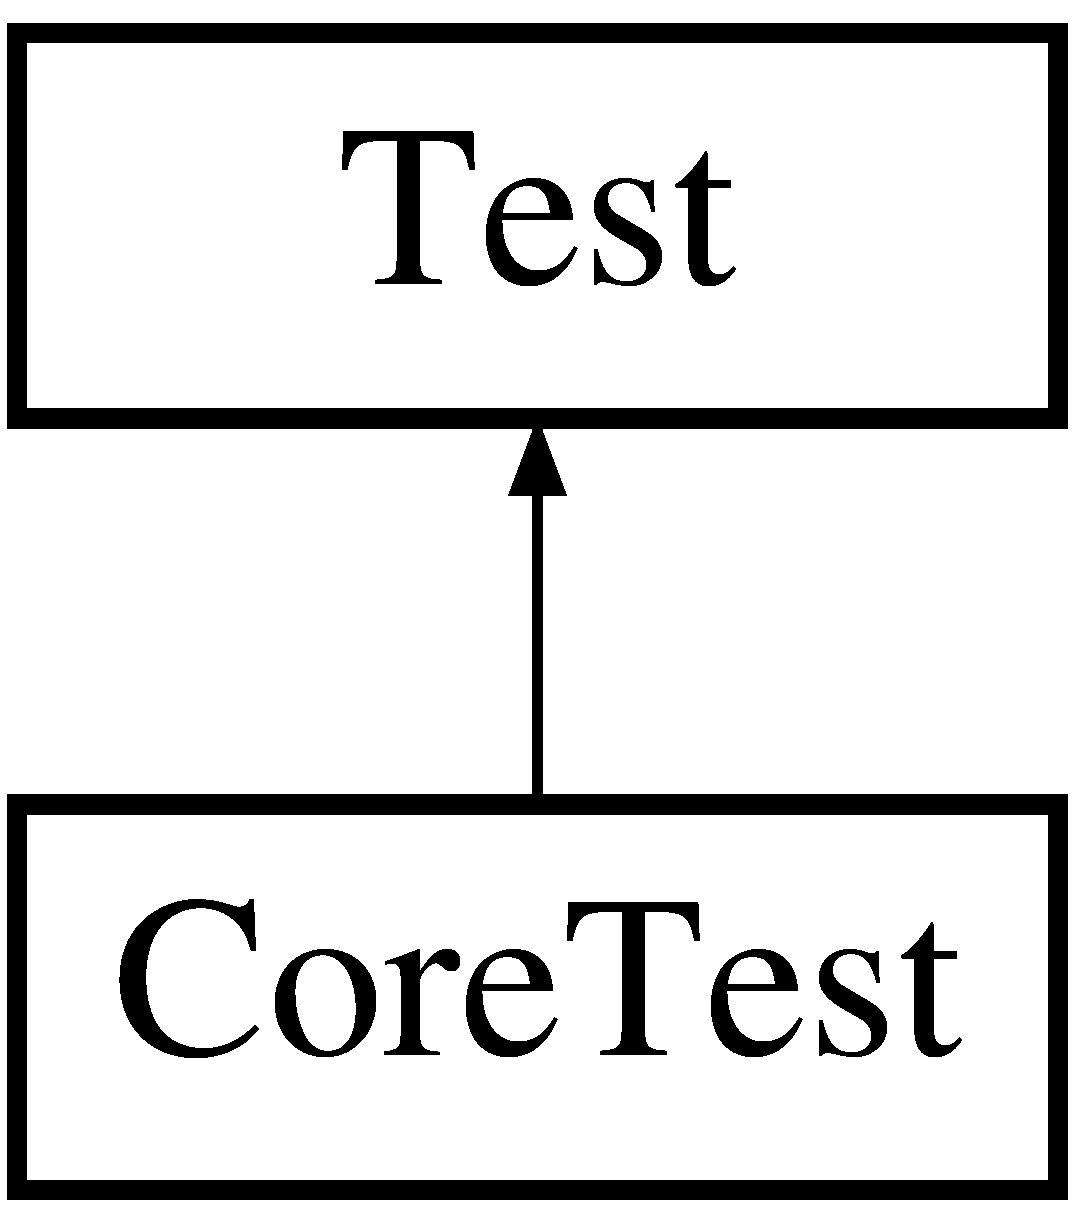
\includegraphics[height=2.000000cm]{classCoreTest}
\end{center}
\end{figure}
\subsection*{Public Member Functions}
\begin{DoxyCompactItemize}
\item 
\mbox{\Hypertarget{classCoreTest_a22a5fdd342d0595ba2569bb389c6828f}\label{classCoreTest_a22a5fdd342d0595ba2569bb389c6828f}} 
virtual void {\bfseries Set\+Up} ()
\item 
\mbox{\Hypertarget{classCoreTest_acc29a8f5c4eb93a6ff01637f81ec4fd9}\label{classCoreTest_acc29a8f5c4eb93a6ff01637f81ec4fd9}} 
virtual void {\bfseries Tear\+Down} ()
\end{DoxyCompactItemize}
\subsection*{Public Attributes}
\begin{DoxyCompactItemize}
\item 
\mbox{\Hypertarget{classCoreTest_a3c5a4de48beffb922c5af71827d33427}\label{classCoreTest_a3c5a4de48beffb922c5af71827d33427}} 
\hyperlink{classSDLMock}{S\+D\+L\+Mock} $\ast$ {\bfseries mock}
\end{DoxyCompactItemize}


\subsection{Detailed Description}


Definition at line 14 of file Core\+Test.\+h.



The documentation for this class was generated from the following file\+:\begin{DoxyCompactItemize}
\item 
/home/skaupper/dev/\+B\+K\+Engine/tests/Core\+Test.\+h\end{DoxyCompactItemize}

\hypertarget{classbkengine_1_1Element}{}\section{bkengine\+:\+:Element Class Reference}
\label{classbkengine_1_1Element}\index{bkengine\+::\+Element@{bkengine\+::\+Element}}
Inheritance diagram for bkengine\+:\+:Element\+:\begin{figure}[H]
\begin{center}
\leavevmode
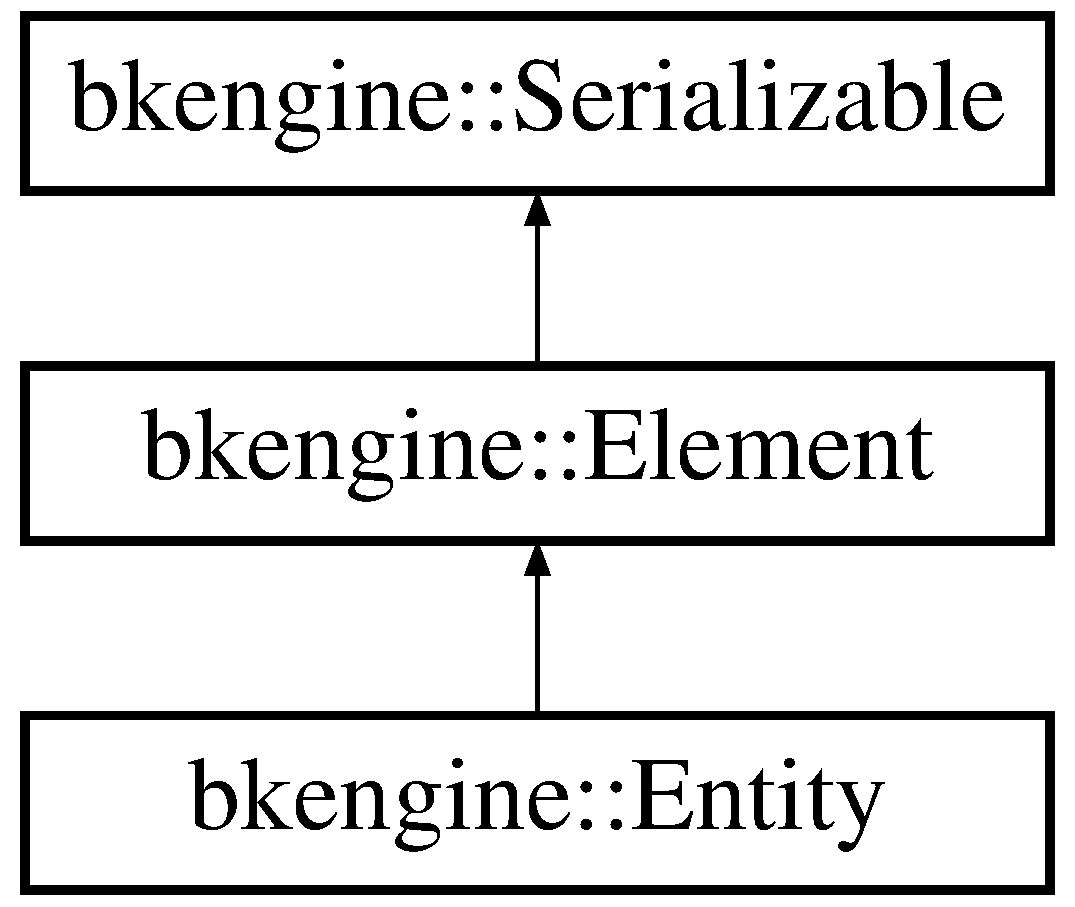
\includegraphics[height=3.000000cm]{classbkengine_1_1Element}
\end{center}
\end{figure}
\subsection*{Public Member Functions}
\begin{DoxyCompactItemize}
\item 
\mbox{\Hypertarget{classbkengine_1_1Element_aeef6831a59bc0362e9364209a96aecb3}\label{classbkengine_1_1Element_aeef6831a59bc0362e9364209a96aecb3}} 
void {\bfseries activate} (unsigned int index)
\item 
\mbox{\Hypertarget{classbkengine_1_1Element_ab2d7e750592b1f05034f2e2238e8f6da}\label{classbkengine_1_1Element_ab2d7e750592b1f05034f2e2238e8f6da}} 
void {\bfseries activate} (const std\+::string \&name)
\item 
\mbox{\Hypertarget{classbkengine_1_1Element_aeb0c71fe0902acf1ab112779b8aabbb7}\label{classbkengine_1_1Element_aeb0c71fe0902acf1ab112779b8aabbb7}} 
bool {\bfseries has\+Animation} (const std\+::string \&name) const
\item 
\mbox{\Hypertarget{classbkengine_1_1Element_aad72daffeb6d69723a01a66eab504d27}\label{classbkengine_1_1Element_aad72daffeb6d69723a01a66eab504d27}} 
bool {\bfseries has\+Animation} (unsigned int index) const
\item 
\mbox{\Hypertarget{classbkengine_1_1Element_a9b106b380f98527c0a06364e99e9701f}\label{classbkengine_1_1Element_a9b106b380f98527c0a06364e99e9701f}} 
void {\bfseries remove\+Animation} (const std\+::string \&name)
\item 
\mbox{\Hypertarget{classbkengine_1_1Element_ad12990a7920262d3011078140a1ce2cc}\label{classbkengine_1_1Element_ad12990a7920262d3011078140a1ce2cc}} 
void {\bfseries remove\+Animation} (unsigned int index)
\item 
\mbox{\Hypertarget{classbkengine_1_1Element_a56be6de0352ac3a0ca487b6f49fed84e}\label{classbkengine_1_1Element_a56be6de0352ac3a0ca487b6f49fed84e}} 
\hyperlink{classbkengine_1_1Animation}{Animation} \& {\bfseries get\+Animation} (const std\+::string \&name)
\item 
\mbox{\Hypertarget{classbkengine_1_1Element_aad7101318ccb2dd833491f1cdd07c13c}\label{classbkengine_1_1Element_aad7101318ccb2dd833491f1cdd07c13c}} 
\hyperlink{classbkengine_1_1Animation}{Animation} \& {\bfseries get\+Animation} (unsigned int index)
\item 
\mbox{\Hypertarget{classbkengine_1_1Element_a78aa2eaf1f376cd3f65278303efb1f30}\label{classbkengine_1_1Element_a78aa2eaf1f376cd3f65278303efb1f30}} 
\hyperlink{classbkengine_1_1Animation}{Animation} \& {\bfseries get\+Current\+Animation} ()
\item 
\mbox{\Hypertarget{classbkengine_1_1Element_a61332cf910adfc845cee4bb9342d09dc}\label{classbkengine_1_1Element_a61332cf910adfc845cee4bb9342d09dc}} 
{\footnotesize template$<$typename T $>$ }\\T \& {\bfseries add\+Animation} (const T \&)
\item 
\mbox{\Hypertarget{classbkengine_1_1Element_a38953a80531b2f444b61b7c400983bf1}\label{classbkengine_1_1Element_a38953a80531b2f444b61b7c400983bf1}} 
{\footnotesize template$<$typename T $>$ }\\T \& {\bfseries add\+Animation} (const std\+::shared\+\_\+ptr$<$ T $>$ \&)
\item 
\mbox{\Hypertarget{classbkengine_1_1Element_a32ae4ca339295c8f78c7e09297f74557}\label{classbkengine_1_1Element_a32ae4ca339295c8f78c7e09297f74557}} 
{\footnotesize template$<$typename T , typename... Params$>$ }\\T \& {\bfseries add\+Animation} (Params...)
\item 
\mbox{\Hypertarget{classbkengine_1_1Element_a8884f71bdf7e36f9354c74db725ab8e1}\label{classbkengine_1_1Element_a8884f71bdf7e36f9354c74db725ab8e1}} 
{\footnotesize template$<$typename T $>$ }\\T \& {\bfseries get\+Animation} (const std\+::string \&name)
\item 
\mbox{\Hypertarget{classbkengine_1_1Element_a459cbd687eb823c2de05923b85ba1a05}\label{classbkengine_1_1Element_a459cbd687eb823c2de05923b85ba1a05}} 
{\footnotesize template$<$typename T $>$ }\\T \& {\bfseries get\+Animation} (unsigned int index)
\item 
\mbox{\Hypertarget{classbkengine_1_1Element_aa35ae3f7cd4d10b3facdebee044ed7df}\label{classbkengine_1_1Element_aa35ae3f7cd4d10b3facdebee044ed7df}} 
{\footnotesize template$<$typename T $>$ }\\T \& {\bfseries get\+Current\+Animation} ()
\item 
\mbox{\Hypertarget{classbkengine_1_1Element_a4c356c014cd8e6e75c7299d30fd4f656}\label{classbkengine_1_1Element_a4c356c014cd8e6e75c7299d30fd4f656}} 
void {\bfseries apply\+Collision\+Box} (const \hyperlink{structbkengine_1_1Rect}{Rect} \&)
\item 
\mbox{\Hypertarget{classbkengine_1_1Element_a665948ae462526e85c3415bc4a787bf9}\label{classbkengine_1_1Element_a665948ae462526e85c3415bc4a787bf9}} 
\hyperlink{structbkengine_1_1Rect}{Rect} {\bfseries get\+Collision\+Box} () const
\item 
\mbox{\Hypertarget{classbkengine_1_1Element_ae1dc97b40cd57da416e872dda8dab6f0}\label{classbkengine_1_1Element_ae1dc97b40cd57da416e872dda8dab6f0}} 
void {\bfseries set\+Render\+Box} (const \hyperlink{structbkengine_1_1Rect}{Rect} \&)
\item 
\mbox{\Hypertarget{classbkengine_1_1Element_ae77ef65af18663617de94580af9105ca}\label{classbkengine_1_1Element_ae77ef65af18663617de94580af9105ca}} 
\hyperlink{structbkengine_1_1Rect}{Rect} {\bfseries get\+Render\+Box} () const
\item 
\mbox{\Hypertarget{classbkengine_1_1Element_a7ecc72f1f593b2b60e24f0aab04fcb30}\label{classbkengine_1_1Element_a7ecc72f1f593b2b60e24f0aab04fcb30}} 
std\+::string {\bfseries get\+Name} () const
\item 
\mbox{\Hypertarget{classbkengine_1_1Element_a7cc283a0caeba6d97159b1073f9b5051}\label{classbkengine_1_1Element_a7cc283a0caeba6d97159b1073f9b5051}} 
{\bfseries Element} (\hyperlink{classbkengine_1_1Scene}{Scene} $\ast$parent\+Scene=nullptr, const std\+::string \&name=\char`\"{}\char`\"{}, const \hyperlink{structbkengine_1_1Rect}{Rect} \&renderbox=\hyperlink{structbkengine_1_1Rect}{Rect}(), int collision\+Layer=-\/1)
\item 
\mbox{\Hypertarget{classbkengine_1_1Element_a11f523eef968855c8780e47e1dc7b977}\label{classbkengine_1_1Element_a11f523eef968855c8780e47e1dc7b977}} 
virtual void {\bfseries setup\+Environment} ()
\item 
\mbox{\Hypertarget{classbkengine_1_1Element_aafdd4a5e2af3f78c41cb5c429c72433f}\label{classbkengine_1_1Element_aafdd4a5e2af3f78c41cb5c429c72433f}} 
virtual void {\bfseries setup\+Animations} ()
\item 
\mbox{\Hypertarget{classbkengine_1_1Element_a9cd4b952fd8b635787896d7d62c303e3}\label{classbkengine_1_1Element_a9cd4b952fd8b635787896d7d62c303e3}} 
virtual void {\bfseries on\+Render} (const \hyperlink{structbkengine_1_1Rect}{Rect} \&parent\+Rect=\hyperlink{structbkengine_1_1Rect}{Rect}())
\item 
\mbox{\Hypertarget{classbkengine_1_1Element_ac366eebb8a84c35989fd347c988c0737}\label{classbkengine_1_1Element_ac366eebb8a84c35989fd347c988c0737}} 
virtual void {\bfseries on\+Loop} ()
\item 
\mbox{\Hypertarget{classbkengine_1_1Element_ab1ad430710a064b28a70b42e4b59a470}\label{classbkengine_1_1Element_ab1ad430710a064b28a70b42e4b59a470}} 
virtual bool {\bfseries on\+Event} (const \hyperlink{classbkengine_1_1Event}{Event} \&)
\item 
\mbox{\Hypertarget{classbkengine_1_1Element_a7ce83303f60b5f5b3d85e70ca58923fc}\label{classbkengine_1_1Element_a7ce83303f60b5f5b3d85e70ca58923fc}} 
void {\bfseries clear} ()
\item 
\mbox{\Hypertarget{classbkengine_1_1Element_a84c3ed3c1f65adcff1febfcaccb6dfbc}\label{classbkengine_1_1Element_a84c3ed3c1f65adcff1febfcaccb6dfbc}} 
virtual void {\bfseries deserialize} (const Json\+::\+Value \&) override
\item 
\mbox{\Hypertarget{classbkengine_1_1Element_a8c82eb831b009ca1c25637402c1d6c42}\label{classbkengine_1_1Element_a8c82eb831b009ca1c25637402c1d6c42}} 
virtual Json\+::\+Value {\bfseries serialize} () const override
\item 
\mbox{\Hypertarget{classbkengine_1_1Element_a6a35edffac23310366fe0013b6a22ae8}\label{classbkengine_1_1Element_a6a35edffac23310366fe0013b6a22ae8}} 
{\footnotesize template$<$typename T $>$ }\\T \& {\bfseries add\+Animation} (const T \&animation)
\item 
\mbox{\Hypertarget{classbkengine_1_1Element_a053bf20ca1e7914d5a51ed1fa84b1bf5}\label{classbkengine_1_1Element_a053bf20ca1e7914d5a51ed1fa84b1bf5}} 
{\footnotesize template$<$typename T $>$ }\\T \& {\bfseries add\+Animation} (const std\+::shared\+\_\+ptr$<$ T $>$ \&animation)
\item 
\mbox{\Hypertarget{classbkengine_1_1Element_a2f51235601148d0fa26d434f1c75d6e9}\label{classbkengine_1_1Element_a2f51235601148d0fa26d434f1c75d6e9}} 
{\footnotesize template$<$typename T , typename... Params$>$ }\\T \& {\bfseries add\+Animation} (Params... params)
\item 
\mbox{\Hypertarget{classbkengine_1_1Element_a405c00e434c1a27f79704b0ee58da4d4}\label{classbkengine_1_1Element_a405c00e434c1a27f79704b0ee58da4d4}} 
{\footnotesize template$<$typename T $>$ }\\T \& {\bfseries get\+Animation} (const std\+::string \&name)
\item 
\mbox{\Hypertarget{classbkengine_1_1Element_ab0c456bd25eaaa697d7485a46b1db5f4}\label{classbkengine_1_1Element_ab0c456bd25eaaa697d7485a46b1db5f4}} 
{\footnotesize template$<$typename T $>$ }\\T \& {\bfseries get\+Animation} (unsigned int index)
\item 
\mbox{\Hypertarget{classbkengine_1_1Element_acdf66af78486ded77d87edd4773b9157}\label{classbkengine_1_1Element_acdf66af78486ded77d87edd4773b9157}} 
{\footnotesize template$<$typename T $>$ }\\T \& {\bfseries get\+Current\+Animation} ()
\end{DoxyCompactItemize}
\subsection*{Friends}
\begin{DoxyCompactItemize}
\item 
\mbox{\Hypertarget{classbkengine_1_1Element_a032858ae1fe02d2d1170981c2af2d67c}\label{classbkengine_1_1Element_a032858ae1fe02d2d1170981c2af2d67c}} 
class {\bfseries Scene}
\end{DoxyCompactItemize}


\subsection{Detailed Description}


Definition at line 16 of file Element.\+h.



The documentation for this class was generated from the following files\+:\begin{DoxyCompactItemize}
\item 
/home/skaupper/dev/\+B\+K\+Engine/include/bkengine/Element.\+h\item 
/home/skaupper/dev/\+B\+K\+Engine/include/bkengine/templates/Element\+\_\+templates.\+h\item 
/home/skaupper/dev/\+B\+K\+Engine/src/Element.\+cpp\end{DoxyCompactItemize}

\hypertarget{classbkengine_1_1Entity}{}\section{bkengine\+:\+:Entity Class Reference}
\label{classbkengine_1_1Entity}\index{bkengine\+::\+Entity@{bkengine\+::\+Entity}}
Inheritance diagram for bkengine\+:\+:Entity\+:\begin{figure}[H]
\begin{center}
\leavevmode
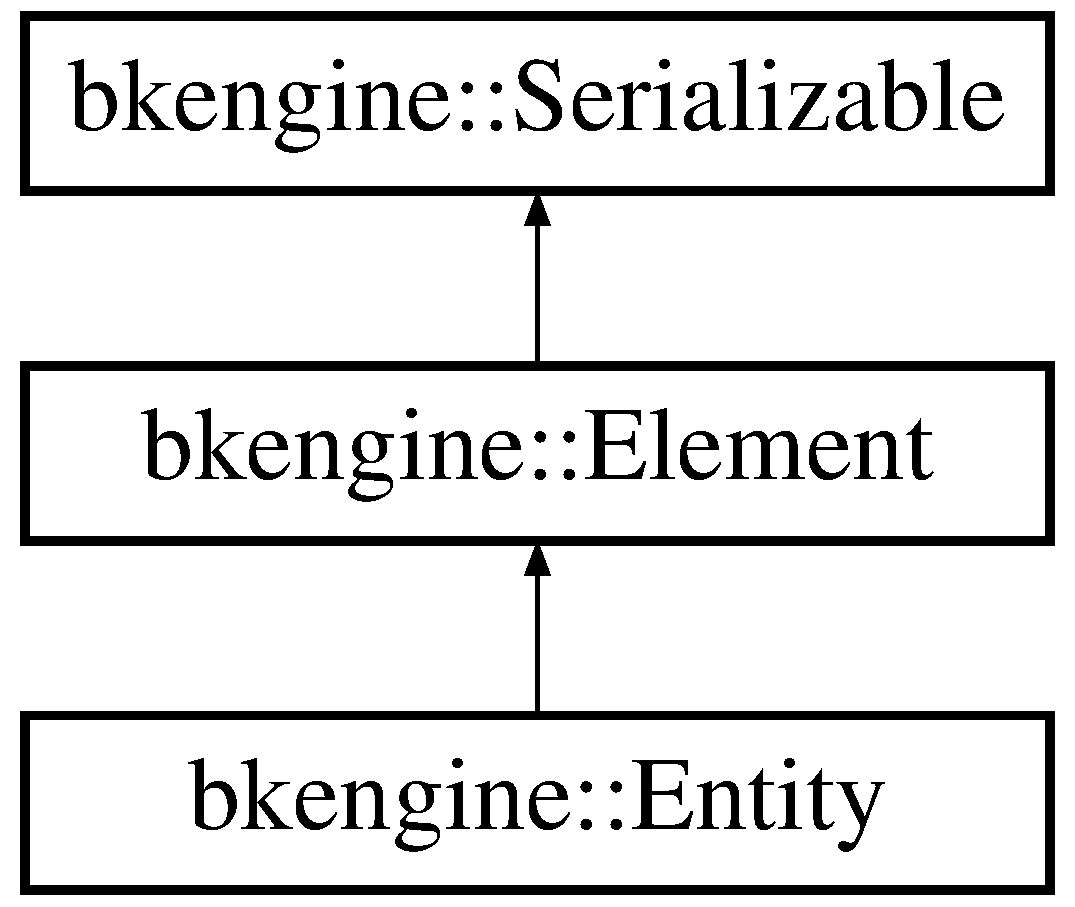
\includegraphics[height=3.000000cm]{classbkengine_1_1Entity}
\end{center}
\end{figure}
\subsection*{Public Member Functions}
\begin{DoxyCompactItemize}
\item 
\mbox{\Hypertarget{classbkengine_1_1Entity_a18c1a6a4603097391f9e64fd0494fd3a}\label{classbkengine_1_1Entity_a18c1a6a4603097391f9e64fd0494fd3a}} 
void {\bfseries move} (float x, float y)
\item 
\mbox{\Hypertarget{classbkengine_1_1Entity_a86f9bb9793c9eb5b51bbddbd5d00f1f7}\label{classbkengine_1_1Entity_a86f9bb9793c9eb5b51bbddbd5d00f1f7}} 
void {\bfseries move\+To} (float x, float y)
\item 
\mbox{\Hypertarget{classbkengine_1_1Entity_ada24ed7c2cda7f426493b053e61c7aad}\label{classbkengine_1_1Entity_ada24ed7c2cda7f426493b053e61c7aad}} 
bool {\bfseries collides\+With} ()
\item 
\mbox{\Hypertarget{classbkengine_1_1Entity_a0865cb6987b1c269cfeeef8e83156052}\label{classbkengine_1_1Entity_a0865cb6987b1c269cfeeef8e83156052}} 
virtual bool {\bfseries collides\+With} (const \hyperlink{classbkengine_1_1Element}{Element} \&other) const
\end{DoxyCompactItemize}


\subsection{Detailed Description}


Definition at line 11 of file Entity.\+h.



The documentation for this class was generated from the following files\+:\begin{DoxyCompactItemize}
\item 
/home/skaupper/dev/\+B\+K\+Engine/include/bkengine/Entity.\+h\item 
/home/skaupper/dev/\+B\+K\+Engine/src/Entity.\+cpp\end{DoxyCompactItemize}

\hypertarget{classbkengine_1_1Event}{}\section{bkengine\+:\+:Event Class Reference}
\label{classbkengine_1_1Event}\index{bkengine\+::\+Event@{bkengine\+::\+Event}}
\subsection*{Public Member Functions}
\begin{DoxyCompactItemize}
\item 
\mbox{\Hypertarget{classbkengine_1_1Event_ae8b35bf9237b74824194f87128e4fdab}\label{classbkengine_1_1Event_ae8b35bf9237b74824194f87128e4fdab}} 
{\bfseries Event} (const \hyperlink{classbkengine_1_1Event}{Event} \&event)
\item 
\mbox{\Hypertarget{classbkengine_1_1Event_af37245d358792cdef34ff4c76c74c022}\label{classbkengine_1_1Event_af37245d358792cdef34ff4c76c74c022}} 
\hyperlink{classbkengine_1_1Event}{Event} \& {\bfseries operator=} (const \hyperlink{classbkengine_1_1Event}{Event} \&event)
\end{DoxyCompactItemize}
\subsection*{Public Attributes}
\begin{DoxyCompactItemize}
\item 
\mbox{\Hypertarget{classbkengine_1_1Event_a8145facb5263afa33ca9f9e800ce5118}\label{classbkengine_1_1Event_a8145facb5263afa33ca9f9e800ce5118}} 
Event\+Type {\bfseries type} = Event\+Type\+::\+U\+N\+K\+N\+O\+WN
\item 
uint32\+\_\+t {\bfseries time\+Stamp}
\item 
\mbox{\Hypertarget{classbkengine_1_1Event_a05484dcb868d79f253c09976f924e751}\label{classbkengine_1_1Event_a05484dcb868d79f253c09976f924e751}} 
uint32\+\_\+t {\bfseries window\+Id} = 0
\item 
\mbox{\Hypertarget{classbkengine_1_1Event_aadc58f0db80bf22bcc5fca0e7fa18ad9}\label{classbkengine_1_1Event_aadc58f0db80bf22bcc5fca0e7fa18ad9}} 
\begin{tabbing}
xx\=xx\=xx\=xx\=xx\=xx\=xx\=xx\=xx\=\kill
union \{\\
\>\hyperlink{structbkengine_1_1KeyboardEvent}{KeyboardEvent} {\bfseries keyboard}\\
\>\hyperlink{structbkengine_1_1MouseEvent}{MouseEvent} {\bfseries mouse}\\
\>\hyperlink{structbkengine_1_1MotionEvent}{MotionEvent} {\bfseries motion}\\
\>\hyperlink{structbkengine_1_1WheelEvent}{WheelEvent} {\bfseries wheel}\\
\>\hyperlink{structbkengine_1_1WindowEvent}{WindowEvent} {\bfseries window}\\
\}; \\

\end{tabbing}\end{DoxyCompactItemize}


\subsection{Detailed Description}


Definition at line 87 of file Event.\+h.



\subsection{Member Data Documentation}
\mbox{\Hypertarget{classbkengine_1_1Event_a4d84f11e0495c24c8056653b33e62d3e}\label{classbkengine_1_1Event_a4d84f11e0495c24c8056653b33e62d3e}} 
\index{bkengine\+::\+Event@{bkengine\+::\+Event}!time\+Stamp@{time\+Stamp}}
\index{time\+Stamp@{time\+Stamp}!bkengine\+::\+Event@{bkengine\+::\+Event}}
\subsubsection{\texorpdfstring{time\+Stamp}{timeStamp}}
{\footnotesize\ttfamily uint32\+\_\+t bkengine\+::\+Event\+::time\+Stamp}

{\bfseries Initial value\+:}
\begin{DoxyCode}
= std::chrono::duration\_cast<std::chrono::seconds>
                                 (std::chrono::system\_clock::now().time\_since\_epoch()).count()
\end{DoxyCode}


Definition at line 96 of file Event.\+h.



The documentation for this class was generated from the following files\+:\begin{DoxyCompactItemize}
\item 
/home/skaupper/dev/\+B\+K\+Engine/include/bkengine/Event.\+h\item 
/home/skaupper/dev/\+B\+K\+Engine/src/Event.\+cpp\end{DoxyCompactItemize}

\hypertarget{classbkengine_1_1EventInterface}{}\section{bkengine\+:\+:Event\+Interface Class Reference}
\label{classbkengine_1_1EventInterface}\index{bkengine\+::\+Event\+Interface@{bkengine\+::\+Event\+Interface}}
Inheritance diagram for bkengine\+:\+:Event\+Interface\+:\begin{figure}[H]
\begin{center}
\leavevmode
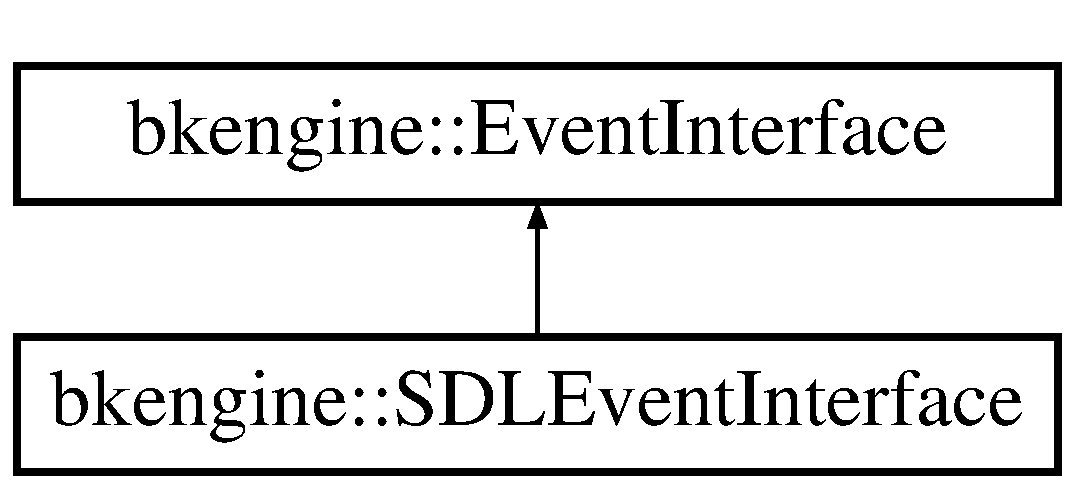
\includegraphics[height=2.000000cm]{classbkengine_1_1EventInterface}
\end{center}
\end{figure}
\subsection*{Public Member Functions}
\begin{DoxyCompactItemize}
\item 
\mbox{\Hypertarget{classbkengine_1_1EventInterface_ab4a68c0c0ca6b55d538afbbb14445345}\label{classbkengine_1_1EventInterface_ab4a68c0c0ca6b55d538afbbb14445345}} 
virtual bool {\bfseries ready} ()=0
\item 
\mbox{\Hypertarget{classbkengine_1_1EventInterface_a2fdf99cc68cc5e12f03cc73634e7b500}\label{classbkengine_1_1EventInterface_a2fdf99cc68cc5e12f03cc73634e7b500}} 
virtual \hyperlink{classbkengine_1_1Event}{Event} {\bfseries poll} ()=0
\end{DoxyCompactItemize}


\subsection{Detailed Description}


Definition at line 8 of file Event\+Interface.\+h.



The documentation for this class was generated from the following file\+:\begin{DoxyCompactItemize}
\item 
/home/skaupper/dev/\+B\+K\+Engine/include/bkengine/Event\+Interface.\+h\end{DoxyCompactItemize}

\hypertarget{classbkengine_1_1Fonts}{}\section{bkengine\+:\+:Fonts Class Reference}
\label{classbkengine_1_1Fonts}\index{bkengine\+::\+Fonts@{bkengine\+::\+Fonts}}
\subsection*{Static Public Member Functions}
\begin{DoxyCompactItemize}
\item 
\mbox{\Hypertarget{classbkengine_1_1Fonts_a5690d3d95ae99ebab8f5598a81fce92f}\label{classbkengine_1_1Fonts_a5690d3d95ae99ebab8f5598a81fce92f}} 
static T\+T\+F\+\_\+\+Font $\ast$ {\bfseries register\+Font} (const std\+::string \&font\+File, int size, const std\+::string \&font\+Name=\char`\"{}\char`\"{})
\item 
\mbox{\Hypertarget{classbkengine_1_1Fonts_a87f4f938ffe851562cf930206daf8898}\label{classbkengine_1_1Fonts_a87f4f938ffe851562cf930206daf8898}} 
static T\+T\+F\+\_\+\+Font $\ast$ {\bfseries get\+Font} (const std\+::string \&font\+Name, int size)
\item 
\mbox{\Hypertarget{classbkengine_1_1Fonts_a2462498df69b120920e5258ad9c8f08d}\label{classbkengine_1_1Fonts_a2462498df69b120920e5258ad9c8f08d}} 
static void {\bfseries release\+Font} (const std\+::string \&font\+Name, int size)
\end{DoxyCompactItemize}
\subsection*{Friends}
\begin{DoxyCompactItemize}
\item 
\mbox{\Hypertarget{classbkengine_1_1Fonts_aa2fab026580d6f14280c2ffb8063a314}\label{classbkengine_1_1Fonts_aa2fab026580d6f14280c2ffb8063a314}} 
class {\bfseries Game}
\end{DoxyCompactItemize}


\subsection{Detailed Description}


Definition at line 15 of file Fonts.\+h.



The documentation for this class was generated from the following files\+:\begin{DoxyCompactItemize}
\item 
/home/skaupper/dev/\+B\+K\+Engine/include/bkengine/Fonts.\+h\item 
/home/skaupper/dev/\+B\+K\+Engine/src/Fonts.\+cpp\end{DoxyCompactItemize}

\hypertarget{classbkengine_1_1Game}{}\section{bkengine\+:\+:Game Class Reference}
\label{classbkengine_1_1Game}\index{bkengine\+::\+Game@{bkengine\+::\+Game}}
Inheritance diagram for bkengine\+:\+:Game\+:\begin{figure}[H]
\begin{center}
\leavevmode
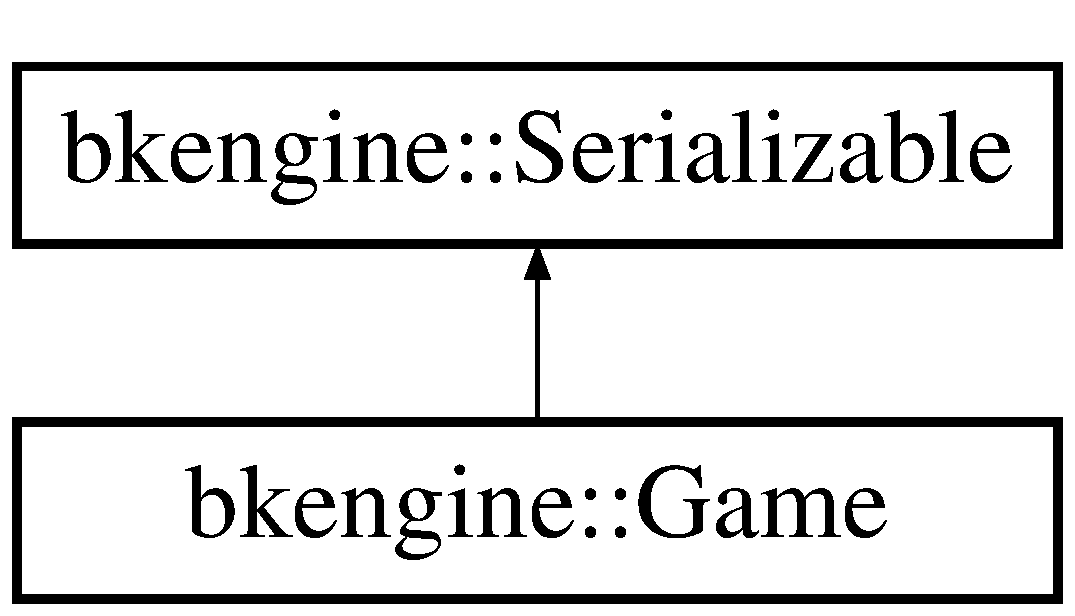
\includegraphics[height=2.000000cm]{classbkengine_1_1Game}
\end{center}
\end{figure}
\subsection*{Public Member Functions}
\begin{DoxyCompactItemize}
\item 
\mbox{\Hypertarget{classbkengine_1_1Game_a4c31e4b00495c28530575b845d2c6384}\label{classbkengine_1_1Game_a4c31e4b00495c28530575b845d2c6384}} 
void {\bfseries activate} (const std\+::string \&name)
\item 
\mbox{\Hypertarget{classbkengine_1_1Game_a1916cb138d297d1a8e5c1c2b31843309}\label{classbkengine_1_1Game_a1916cb138d297d1a8e5c1c2b31843309}} 
void {\bfseries activate} (unsigned int index)
\item 
\mbox{\Hypertarget{classbkengine_1_1Game_acba38c7030021f866cff9a1df67ee00d}\label{classbkengine_1_1Game_acba38c7030021f866cff9a1df67ee00d}} 
bool {\bfseries has\+Scene} (const std\+::string \&name) const
\item 
\mbox{\Hypertarget{classbkengine_1_1Game_a74e4a0a4ec36b5282e5f0cddfa786f99}\label{classbkengine_1_1Game_a74e4a0a4ec36b5282e5f0cddfa786f99}} 
bool {\bfseries has\+Scene} (unsigned int index) const
\item 
\mbox{\Hypertarget{classbkengine_1_1Game_a32a365e70c7e4afeb43359a8e66b5d08}\label{classbkengine_1_1Game_a32a365e70c7e4afeb43359a8e66b5d08}} 
void {\bfseries remove\+Scene} (const std\+::string \&name)
\item 
\mbox{\Hypertarget{classbkengine_1_1Game_afe4b932a5b3d331ea48f63cb9b48e6aa}\label{classbkengine_1_1Game_afe4b932a5b3d331ea48f63cb9b48e6aa}} 
void {\bfseries remove\+Scene} (unsigned int index)
\item 
\mbox{\Hypertarget{classbkengine_1_1Game_a486a485a7ce8122dff0d63f439081ec0}\label{classbkengine_1_1Game_a486a485a7ce8122dff0d63f439081ec0}} 
\hyperlink{classbkengine_1_1Scene}{Scene} \& {\bfseries get\+Scene} (const std\+::string \&name)
\item 
\mbox{\Hypertarget{classbkengine_1_1Game_a8b9e4c8580e8b183138e37617efa4db4}\label{classbkengine_1_1Game_a8b9e4c8580e8b183138e37617efa4db4}} 
\hyperlink{classbkengine_1_1Scene}{Scene} \& {\bfseries get\+Scene} (unsigned int index)
\item 
\mbox{\Hypertarget{classbkengine_1_1Game_ad9d677a0c5648f37961af294d12ef407}\label{classbkengine_1_1Game_ad9d677a0c5648f37961af294d12ef407}} 
\hyperlink{classbkengine_1_1Scene}{Scene} \& {\bfseries get\+Current\+Scene} ()
\item 
\mbox{\Hypertarget{classbkengine_1_1Game_ae10f3f55a157ea67aa44b2826d214757}\label{classbkengine_1_1Game_ae10f3f55a157ea67aa44b2826d214757}} 
{\footnotesize template$<$typename T $>$ }\\T \& {\bfseries add\+Scene} (const T \&)
\item 
\mbox{\Hypertarget{classbkengine_1_1Game_a42a7df337b004ba8e090c4cad4389565}\label{classbkengine_1_1Game_a42a7df337b004ba8e090c4cad4389565}} 
{\footnotesize template$<$typename T $>$ }\\T \& {\bfseries add\+Scene} (const std\+::shared\+\_\+ptr$<$ T $>$ \&)
\item 
\mbox{\Hypertarget{classbkengine_1_1Game_af3c7c7aa11150d386c45e8085f2407d7}\label{classbkengine_1_1Game_af3c7c7aa11150d386c45e8085f2407d7}} 
{\footnotesize template$<$typename T , typename... Params$>$ }\\T \& {\bfseries add\+Scene} (Params...)
\item 
\mbox{\Hypertarget{classbkengine_1_1Game_a7f20847c5da4e2ddd51273519e11df16}\label{classbkengine_1_1Game_a7f20847c5da4e2ddd51273519e11df16}} 
{\footnotesize template$<$typename T $>$ }\\T \& {\bfseries get\+Scene} (const std\+::string \&name)
\item 
\mbox{\Hypertarget{classbkengine_1_1Game_aa7a913a564504cbcaf7c7d442d1fea92}\label{classbkengine_1_1Game_aa7a913a564504cbcaf7c7d442d1fea92}} 
{\footnotesize template$<$typename T $>$ }\\T \& {\bfseries get\+Scene} (unsigned int index)
\item 
\mbox{\Hypertarget{classbkengine_1_1Game_a719d3981be6fa96b07310346311c2413}\label{classbkengine_1_1Game_a719d3981be6fa96b07310346311c2413}} 
{\footnotesize template$<$typename T $>$ }\\T \& {\bfseries get\+Current\+Scene} ()
\item 
\mbox{\Hypertarget{classbkengine_1_1Game_a5b1374495ef9f549c88251d3d930cc12}\label{classbkengine_1_1Game_a5b1374495ef9f549c88251d3d930cc12}} 
bool {\bfseries set\+Icon} (const std\+::string \&icon\+Path)
\item 
\mbox{\Hypertarget{classbkengine_1_1Game_a7494363174008a772d245c20f31b2a19}\label{classbkengine_1_1Game_a7494363174008a772d245c20f31b2a19}} 
void {\bfseries resize\+Window} (int window\+Width, int window\+Height)
\item 
\mbox{\Hypertarget{classbkengine_1_1Game_a2a253152712dc78d5f280badeb34ce3c}\label{classbkengine_1_1Game_a2a253152712dc78d5f280badeb34ce3c}} 
void {\bfseries set\+Window\+Title} (const std\+::string \&)
\item 
\mbox{\Hypertarget{classbkengine_1_1Game_a1480bc58570c9fa4696a642ebe441d7e}\label{classbkengine_1_1Game_a1480bc58570c9fa4696a642ebe441d7e}} 
{\footnotesize template$<$typename T $>$ }\\void {\bfseries set\+Event\+Interface} ()
\item 
\mbox{\Hypertarget{classbkengine_1_1Game_a4c86f004e97fe295c87ea2d756cf9793}\label{classbkengine_1_1Game_a4c86f004e97fe295c87ea2d756cf9793}} 
{\footnotesize template$<$typename T $>$ }\\void {\bfseries set\+Settings\+Interface} ()
\item 
\mbox{\Hypertarget{classbkengine_1_1Game_a03800577e8e89c0370a6e29d62c5bacf}\label{classbkengine_1_1Game_a03800577e8e89c0370a6e29d62c5bacf}} 
std\+::shared\+\_\+ptr$<$ \hyperlink{classbkengine_1_1SettingsInterface}{Settings\+Interface} $>$ {\bfseries get\+Settings\+Interface} ()
\item 
\mbox{\Hypertarget{classbkengine_1_1Game_a91cbdf7dd5a500e2f3fe44cfc5c9b7ba}\label{classbkengine_1_1Game_a91cbdf7dd5a500e2f3fe44cfc5c9b7ba}} 
{\bfseries Game} (int width, int height, const std\+::string \&title)
\item 
\mbox{\Hypertarget{classbkengine_1_1Game_af69eb7d8cc53c238a87d290841951525}\label{classbkengine_1_1Game_af69eb7d8cc53c238a87d290841951525}} 
{\footnotesize template$<$typename T $>$ }\\T \& {\bfseries get\+Data} (const std\+::string \&name)
\item 
\mbox{\Hypertarget{classbkengine_1_1Game_ac9f317fa3194c88239b86a514908bf11}\label{classbkengine_1_1Game_ac9f317fa3194c88239b86a514908bf11}} 
{\footnotesize template$<$typename T $>$ }\\T \& {\bfseries add\+Data} (const std\+::string \&name)
\item 
\mbox{\Hypertarget{classbkengine_1_1Game_a942d8db592cb45378088f315aef0bc21}\label{classbkengine_1_1Game_a942d8db592cb45378088f315aef0bc21}} 
bool {\bfseries has\+Data} (const std\+::string \&name)
\item 
\mbox{\Hypertarget{classbkengine_1_1Game_a1ab78f5ed0d5ea879157357cf2fb2afa}\label{classbkengine_1_1Game_a1ab78f5ed0d5ea879157357cf2fb2afa}} 
void {\bfseries run} ()
\item 
\mbox{\Hypertarget{classbkengine_1_1Game_a17fbb36fd4a2085f9ff4f1fa93d7d08b}\label{classbkengine_1_1Game_a17fbb36fd4a2085f9ff4f1fa93d7d08b}} 
void {\bfseries stop} ()
\item 
\mbox{\Hypertarget{classbkengine_1_1Game_a25f39d006ed6b37397d06cb6f951c33f}\label{classbkengine_1_1Game_a25f39d006ed6b37397d06cb6f951c33f}} 
virtual void {\bfseries setup\+Environment} ()
\item 
\mbox{\Hypertarget{classbkengine_1_1Game_a4a6cdd8a4420d3b678b69c3648bb4a50}\label{classbkengine_1_1Game_a4a6cdd8a4420d3b678b69c3648bb4a50}} 
virtual void {\bfseries setup\+Scenes} ()
\item 
\mbox{\Hypertarget{classbkengine_1_1Game_a3729fd20b2303995d17f2aab824c55ff}\label{classbkengine_1_1Game_a3729fd20b2303995d17f2aab824c55ff}} 
virtual void {\bfseries teardown} ()
\item 
\mbox{\Hypertarget{classbkengine_1_1Game_a8ba8d7bcda356ed584dc445184320ff7}\label{classbkengine_1_1Game_a8ba8d7bcda356ed584dc445184320ff7}} 
void {\bfseries clear} ()
\item 
\mbox{\Hypertarget{classbkengine_1_1Game_ac6f616f1adabfb8622df30edbb63e7e7}\label{classbkengine_1_1Game_ac6f616f1adabfb8622df30edbb63e7e7}} 
virtual void {\bfseries deserialize} (const Json\+::\+Value \&) override
\item 
\mbox{\Hypertarget{classbkengine_1_1Game_a02fd84a6e0f0dfc82f360738581f9eed}\label{classbkengine_1_1Game_a02fd84a6e0f0dfc82f360738581f9eed}} 
virtual Json\+::\+Value {\bfseries serialize} () const override
\item 
\mbox{\Hypertarget{classbkengine_1_1Game_a64bd2346dbaa1bc5e3929f906ed94d95}\label{classbkengine_1_1Game_a64bd2346dbaa1bc5e3929f906ed94d95}} 
{\footnotesize template$<$typename T $>$ }\\T {\bfseries create} (int width, int height, const std\+::string \&title)
\item 
\mbox{\Hypertarget{classbkengine_1_1Game_abf8ff1761ffb25fe79851b1fcfdc903d}\label{classbkengine_1_1Game_abf8ff1761ffb25fe79851b1fcfdc903d}} 
{\footnotesize template$<$typename T $>$ }\\T \& {\bfseries add\+Scene} (const T \&scene)
\item 
\mbox{\Hypertarget{classbkengine_1_1Game_ac619f04cd598a677c7e1e9c6750401b6}\label{classbkengine_1_1Game_ac619f04cd598a677c7e1e9c6750401b6}} 
{\footnotesize template$<$typename T $>$ }\\T \& {\bfseries add\+Scene} (const std\+::shared\+\_\+ptr$<$ T $>$ \&scene)
\item 
\mbox{\Hypertarget{classbkengine_1_1Game_ad4c1a8a7c88ff209cb575bcc978a7d47}\label{classbkengine_1_1Game_ad4c1a8a7c88ff209cb575bcc978a7d47}} 
{\footnotesize template$<$typename T , typename... Params$>$ }\\T \& {\bfseries add\+Scene} (Params... params)
\item 
\mbox{\Hypertarget{classbkengine_1_1Game_af33a446745d9e394b4ad4cf9fe7a6570}\label{classbkengine_1_1Game_af33a446745d9e394b4ad4cf9fe7a6570}} 
{\footnotesize template$<$typename T $>$ }\\T \& {\bfseries get\+Scene} (const std\+::string \&name)
\item 
\mbox{\Hypertarget{classbkengine_1_1Game_a19c505fb0c56f420f44366e16d69b85b}\label{classbkengine_1_1Game_a19c505fb0c56f420f44366e16d69b85b}} 
{\footnotesize template$<$typename T $>$ }\\T \& {\bfseries get\+Scene} (unsigned int index)
\item 
\mbox{\Hypertarget{classbkengine_1_1Game_a7a1bc30c47d3df980851633e99234161}\label{classbkengine_1_1Game_a7a1bc30c47d3df980851633e99234161}} 
{\footnotesize template$<$typename T $>$ }\\T \& {\bfseries get\+Current\+Scene} ()
\item 
\mbox{\Hypertarget{classbkengine_1_1Game_a1480bc58570c9fa4696a642ebe441d7e}\label{classbkengine_1_1Game_a1480bc58570c9fa4696a642ebe441d7e}} 
{\footnotesize template$<$typename T $>$ }\\void {\bfseries set\+Event\+Interface} ()
\item 
\mbox{\Hypertarget{classbkengine_1_1Game_a4c86f004e97fe295c87ea2d756cf9793}\label{classbkengine_1_1Game_a4c86f004e97fe295c87ea2d756cf9793}} 
{\footnotesize template$<$typename T $>$ }\\void {\bfseries set\+Settings\+Interface} ()
\item 
\mbox{\Hypertarget{classbkengine_1_1Game_ab816313a5cfdf6038b9b75a8c8c58730}\label{classbkengine_1_1Game_ab816313a5cfdf6038b9b75a8c8c58730}} 
{\footnotesize template$<$typename T $>$ }\\T \& {\bfseries get\+Data} (const std\+::string \&name)
\item 
\mbox{\Hypertarget{classbkengine_1_1Game_a9fd1d7e5a1ab1665f318cfc6d4aae057}\label{classbkengine_1_1Game_a9fd1d7e5a1ab1665f318cfc6d4aae057}} 
{\footnotesize template$<$typename T $>$ }\\T \& {\bfseries add\+Data} (const std\+::string \&name)
\end{DoxyCompactItemize}
\subsection*{Static Public Member Functions}
\begin{DoxyCompactItemize}
\item 
\mbox{\Hypertarget{classbkengine_1_1Game_ad1be9a123f4758d1a3ec0a547a82612b}\label{classbkengine_1_1Game_ad1be9a123f4758d1a3ec0a547a82612b}} 
{\footnotesize template$<$typename T $>$ }\\static T {\bfseries create} (int=1024, int=768, const std\+::string \&title=\char`\"{}B\+K\+E\+N\+G\+I\+NE W\+I\+N\+D\+OW\char`\"{})
\end{DoxyCompactItemize}


\subsection{Detailed Description}


Definition at line 21 of file Game.\+h.



The documentation for this class was generated from the following files\+:\begin{DoxyCompactItemize}
\item 
/home/skaupper/dev/\+B\+K\+Engine/include/bkengine/Game.\+h\item 
/home/skaupper/dev/\+B\+K\+Engine/include/bkengine/templates/Game\+\_\+templates.\+h\item 
/home/skaupper/dev/\+B\+K\+Engine/src/Game.\+cpp\end{DoxyCompactItemize}

\hypertarget{classbkengine_1_1GameSerializer}{}\section{bkengine\+:\+:Game\+Serializer Class Reference}
\label{classbkengine_1_1GameSerializer}\index{bkengine\+::\+Game\+Serializer@{bkengine\+::\+Game\+Serializer}}
\subsection*{Public Member Functions}
\begin{DoxyCompactItemize}
\item 
\mbox{\Hypertarget{classbkengine_1_1GameSerializer_af853c4ab4056f5d5ccf56d6afadf976c}\label{classbkengine_1_1GameSerializer_af853c4ab4056f5d5ccf56d6afadf976c}} 
{\footnotesize template$<$$>$ }\\std\+::shared\+\_\+ptr$<$ \hyperlink{classbkengine_1_1Game}{Game} $>$ {\bfseries deserialize} (const Json\+::\+Value \&obj)
\item 
\mbox{\Hypertarget{classbkengine_1_1GameSerializer_a4ca10de97f0c3ca5e69ec3ebc82c98ea}\label{classbkengine_1_1GameSerializer_a4ca10de97f0c3ca5e69ec3ebc82c98ea}} 
{\footnotesize template$<$$>$ }\\std\+::shared\+\_\+ptr$<$ \hyperlink{classbkengine_1_1Scene}{Scene} $>$ {\bfseries deserialize} (const Json\+::\+Value \&obj)
\item 
\mbox{\Hypertarget{classbkengine_1_1GameSerializer_a47ee0a5fab46238fee119f05226bc02b}\label{classbkengine_1_1GameSerializer_a47ee0a5fab46238fee119f05226bc02b}} 
{\footnotesize template$<$$>$ }\\std\+::shared\+\_\+ptr$<$ \hyperlink{classbkengine_1_1Element}{Element} $>$ {\bfseries deserialize} (const Json\+::\+Value \&obj)
\item 
\mbox{\Hypertarget{classbkengine_1_1GameSerializer_a88615bdca14bcb3309e435c677555529}\label{classbkengine_1_1GameSerializer_a88615bdca14bcb3309e435c677555529}} 
{\footnotesize template$<$$>$ }\\std\+::shared\+\_\+ptr$<$ \hyperlink{classbkengine_1_1Animation}{Animation} $>$ {\bfseries deserialize} (const Json\+::\+Value \&obj)
\item 
\mbox{\Hypertarget{classbkengine_1_1GameSerializer_a77c6a2676347b3c51d0596e3b89c09db}\label{classbkengine_1_1GameSerializer_a77c6a2676347b3c51d0596e3b89c09db}} 
{\footnotesize template$<$$>$ }\\std\+::shared\+\_\+ptr$<$ \hyperlink{classbkengine_1_1Texture}{Texture} $>$ {\bfseries deserialize} (const Json\+::\+Value \&obj)
\end{DoxyCompactItemize}
\subsection*{Static Public Member Functions}
\begin{DoxyCompactItemize}
\item 
\mbox{\Hypertarget{classbkengine_1_1GameSerializer_a1eed5a6aa6012dda21172db8b5e8714a}\label{classbkengine_1_1GameSerializer_a1eed5a6aa6012dda21172db8b5e8714a}} 
{\footnotesize template$<$typename T $>$ }\\static std\+::shared\+\_\+ptr$<$ T $>$ {\bfseries deserialize} (const Json\+::\+Value \&obj)
\end{DoxyCompactItemize}


\subsection{Detailed Description}


Definition at line 19 of file Game\+Serializer.\+h.



The documentation for this class was generated from the following files\+:\begin{DoxyCompactItemize}
\item 
/home/skaupper/dev/\+B\+K\+Engine/include/bkengine/Game\+Serializer.\+h\item 
/home/skaupper/dev/\+B\+K\+Engine/src/Game\+Serializer.\+cpp\end{DoxyCompactItemize}

\hypertarget{classbkengine_1_1INISettingsInterface}{}\section{bkengine\+:\+:I\+N\+I\+Settings\+Interface Class Reference}
\label{classbkengine_1_1INISettingsInterface}\index{bkengine\+::\+I\+N\+I\+Settings\+Interface@{bkengine\+::\+I\+N\+I\+Settings\+Interface}}
Inheritance diagram for bkengine\+:\+:I\+N\+I\+Settings\+Interface\+:\begin{figure}[H]
\begin{center}
\leavevmode
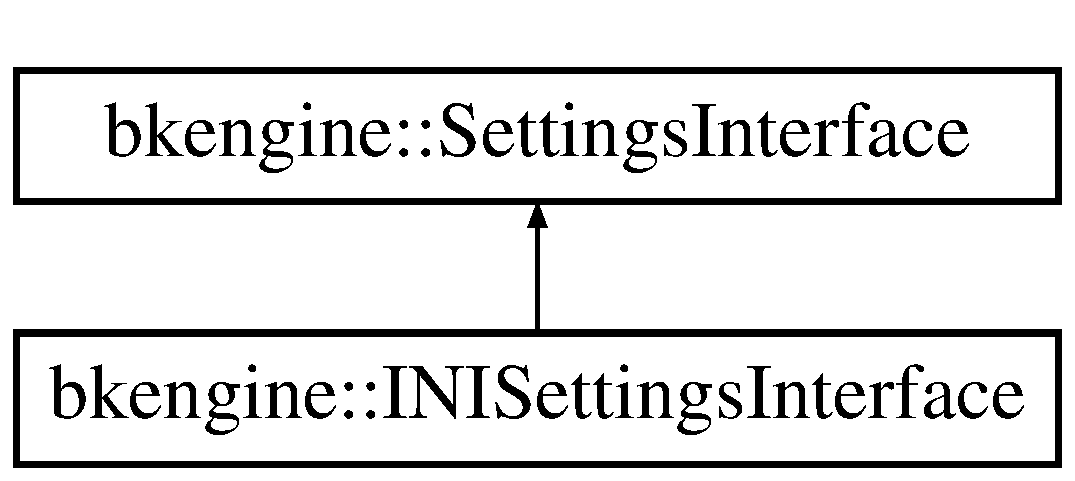
\includegraphics[height=2.000000cm]{classbkengine_1_1INISettingsInterface}
\end{center}
\end{figure}
\subsection*{Public Member Functions}
\begin{DoxyCompactItemize}
\item 
\mbox{\Hypertarget{classbkengine_1_1INISettingsInterface_ad84a5d64d5cc69907d1cbfde8045e5c5}\label{classbkengine_1_1INISettingsInterface_ad84a5d64d5cc69907d1cbfde8045e5c5}} 
virtual void {\bfseries init} () override
\item 
\mbox{\Hypertarget{classbkengine_1_1INISettingsInterface_a08102628fa63304dd60d3dc47a38ea49}\label{classbkengine_1_1INISettingsInterface_a08102628fa63304dd60d3dc47a38ea49}} 
virtual void {\bfseries load\+From\+File} (const std\+::string \&filename) override
\item 
\mbox{\Hypertarget{classbkengine_1_1INISettingsInterface_aab677d0087cf7df2b42a2198c0700ff2}\label{classbkengine_1_1INISettingsInterface_aab677d0087cf7df2b42a2198c0700ff2}} 
virtual void {\bfseries save\+To\+File} (const std\+::string \&filename) const override
\item 
\mbox{\Hypertarget{classbkengine_1_1INISettingsInterface_a8f8c91c1fb425e55422bec1d535e0c4e}\label{classbkengine_1_1INISettingsInterface_a8f8c91c1fb425e55422bec1d535e0c4e}} 
virtual std\+::string {\bfseries get} (const std\+::string \&key) const override
\item 
\mbox{\Hypertarget{classbkengine_1_1INISettingsInterface_acf7c1800ed16171569ec7e29ab4ab371}\label{classbkengine_1_1INISettingsInterface_acf7c1800ed16171569ec7e29ab4ab371}} 
virtual std\+::string {\bfseries remove} (const std\+::string \&key) override
\item 
\mbox{\Hypertarget{classbkengine_1_1INISettingsInterface_aeed7655aa361b07d69d2e97111cd20c7}\label{classbkengine_1_1INISettingsInterface_aeed7655aa361b07d69d2e97111cd20c7}} 
virtual bool {\bfseries has\+Value} (const std\+::string \&key) const override
\item 
\mbox{\Hypertarget{classbkengine_1_1INISettingsInterface_afd51d34f3397ddb3c0f6ce3f7ecdd28d}\label{classbkengine_1_1INISettingsInterface_afd51d34f3397ddb3c0f6ce3f7ecdd28d}} 
virtual void {\bfseries create} (const std\+::string \&key, const std\+::string \&value) override
\item 
\mbox{\Hypertarget{classbkengine_1_1INISettingsInterface_a30c11f0fe030a3bba304962a6b1c77d1}\label{classbkengine_1_1INISettingsInterface_a30c11f0fe030a3bba304962a6b1c77d1}} 
virtual void {\bfseries change} (const std\+::string \&key, const std\+::string \&newvalue) override
\item 
\mbox{\Hypertarget{classbkengine_1_1INISettingsInterface_a58176c5b620d050afc30432a9ac08166}\label{classbkengine_1_1INISettingsInterface_a58176c5b620d050afc30432a9ac08166}} 
virtual uint32\+\_\+t {\bfseries count} () const override
\end{DoxyCompactItemize}


\subsection{Detailed Description}


Definition at line 12 of file I\+N\+I\+Settings\+Interface.\+h.



The documentation for this class was generated from the following files\+:\begin{DoxyCompactItemize}
\item 
/home/skaupper/dev/\+B\+K\+Engine/include/bkengine/I\+N\+I\+Settings\+Interface.\+h\item 
/home/skaupper/dev/\+B\+K\+Engine/src/I\+N\+I\+Settings\+Interface.\+cpp\end{DoxyCompactItemize}

\hypertarget{classbkengine_1_1Key}{}\section{bkengine\+:\+:Key Class Reference}
\label{classbkengine_1_1Key}\index{bkengine\+::\+Key@{bkengine\+::\+Key}}
\subsection*{Public Member Functions}
\begin{DoxyCompactItemize}
\item 
\mbox{\Hypertarget{classbkengine_1_1Key_a54ce3095078f60337098fd48c0af785b}\label{classbkengine_1_1Key_a54ce3095078f60337098fd48c0af785b}} 
{\bfseries Key} (const std\+::string \&key\+String)
\item 
\mbox{\Hypertarget{classbkengine_1_1Key_a8cb85e358786ea8bf137a68fa8e72307}\label{classbkengine_1_1Key_a8cb85e358786ea8bf137a68fa8e72307}} 
bool {\bfseries operator==} (const \hyperlink{classbkengine_1_1Key}{Key} \&) const
\item 
\mbox{\Hypertarget{classbkengine_1_1Key_a2d1bc06b124e7757ac4df2950d2fc108}\label{classbkengine_1_1Key_a2d1bc06b124e7757ac4df2950d2fc108}} 
bool {\bfseries operator!=} (const \hyperlink{classbkengine_1_1Key}{Key} \&) const
\item 
\mbox{\Hypertarget{classbkengine_1_1Key_a13a320efc0b88e3dee46c3413e23351a}\label{classbkengine_1_1Key_a13a320efc0b88e3dee46c3413e23351a}} 
{\bfseries operator const std\+::string} () const
\item 
\mbox{\Hypertarget{classbkengine_1_1Key_ae097454f3d2b400816700e9b6b9738a1}\label{classbkengine_1_1Key_ae097454f3d2b400816700e9b6b9738a1}} 
std\+::string {\bfseries to\+String} () const
\end{DoxyCompactItemize}


\subsection{Detailed Description}


Definition at line 8 of file Keys.\+h.



The documentation for this class was generated from the following files\+:\begin{DoxyCompactItemize}
\item 
/home/skaupper/dev/\+B\+K\+Engine/include/bkengine/Keys.\+h\item 
/home/skaupper/dev/\+B\+K\+Engine/src/Keys.\+cpp\end{DoxyCompactItemize}

\hypertarget{structbkengine_1_1KeyboardEvent}{}\section{bkengine\+:\+:Keyboard\+Event Struct Reference}
\label{structbkengine_1_1KeyboardEvent}\index{bkengine\+::\+Keyboard\+Event@{bkengine\+::\+Keyboard\+Event}}
\subsection*{Public Attributes}
\begin{DoxyCompactItemize}
\item 
\mbox{\Hypertarget{structbkengine_1_1KeyboardEvent_a7512cfbc91f52c63277afc29883f0784}\label{structbkengine_1_1KeyboardEvent_a7512cfbc91f52c63277afc29883f0784}} 
\hyperlink{classbkengine_1_1Key}{Key} {\bfseries key}
\item 
\mbox{\Hypertarget{structbkengine_1_1KeyboardEvent_ae1ef646e201c5bb43506af57b96d104b}\label{structbkengine_1_1KeyboardEvent_ae1ef646e201c5bb43506af57b96d104b}} 
Key\+State {\bfseries state}
\item 
\mbox{\Hypertarget{structbkengine_1_1KeyboardEvent_a7a4e85fd8ad152558feaa9405264a14a}\label{structbkengine_1_1KeyboardEvent_a7a4e85fd8ad152558feaa9405264a14a}} 
bool {\bfseries repeat}
\end{DoxyCompactItemize}


\subsection{Detailed Description}


Definition at line 54 of file Event.\+h.



The documentation for this struct was generated from the following file\+:\begin{DoxyCompactItemize}
\item 
/home/skaupper/dev/\+B\+K\+Engine/include/bkengine/Event.\+h\end{DoxyCompactItemize}

\hypertarget{classbkengine_1_1Keys}{}\section{bkengine\+:\+:Keys Class Reference}
\label{classbkengine_1_1Keys}\index{bkengine\+::\+Keys@{bkengine\+::\+Keys}}
\subsection*{Static Public Attributes}
\begin{DoxyCompactItemize}
\item 
\mbox{\Hypertarget{classbkengine_1_1Keys_addcb4b866148a29c66316aaad8bf6383}\label{classbkengine_1_1Keys_addcb4b866148a29c66316aaad8bf6383}} 
static \hyperlink{classbkengine_1_1Key}{Key} {\bfseries U\+N\+K\+N\+O\+WN}
\item 
\mbox{\Hypertarget{classbkengine_1_1Keys_a774f502aec51497a2e115f4b988eea27}\label{classbkengine_1_1Keys_a774f502aec51497a2e115f4b988eea27}} 
static \hyperlink{classbkengine_1_1Key}{Key} {\bfseries R\+E\+T\+U\+RN}
\item 
\mbox{\Hypertarget{classbkengine_1_1Keys_aae120cdc1dd2c94e5a8d4d67f8144618}\label{classbkengine_1_1Keys_aae120cdc1dd2c94e5a8d4d67f8144618}} 
static \hyperlink{classbkengine_1_1Key}{Key} {\bfseries E\+S\+C\+A\+PE}
\item 
\mbox{\Hypertarget{classbkengine_1_1Keys_a97b56123f742970db534e9dc2f7f0026}\label{classbkengine_1_1Keys_a97b56123f742970db534e9dc2f7f0026}} 
static \hyperlink{classbkengine_1_1Key}{Key} {\bfseries B\+A\+C\+K\+S\+P\+A\+CE}
\item 
\mbox{\Hypertarget{classbkengine_1_1Keys_a33554518bac96b2f2b4441601bee36b4}\label{classbkengine_1_1Keys_a33554518bac96b2f2b4441601bee36b4}} 
static \hyperlink{classbkengine_1_1Key}{Key} {\bfseries T\+AB}
\item 
\mbox{\Hypertarget{classbkengine_1_1Keys_a2530f649d8ec413275a429e11e109596}\label{classbkengine_1_1Keys_a2530f649d8ec413275a429e11e109596}} 
static \hyperlink{classbkengine_1_1Key}{Key} {\bfseries S\+P\+A\+CE}
\item 
\mbox{\Hypertarget{classbkengine_1_1Keys_a06322734d3bb330a58ce47da5b7af579}\label{classbkengine_1_1Keys_a06322734d3bb330a58ce47da5b7af579}} 
static \hyperlink{classbkengine_1_1Key}{Key} {\bfseries C\+A\+P\+S\+L\+O\+CK}
\item 
\mbox{\Hypertarget{classbkengine_1_1Keys_a958a175e1b13f779c8e0f878066cd81a}\label{classbkengine_1_1Keys_a958a175e1b13f779c8e0f878066cd81a}} 
static \hyperlink{classbkengine_1_1Key}{Key} {\bfseries Z\+E\+RO}
\item 
\mbox{\Hypertarget{classbkengine_1_1Keys_ac4fab41f5e4973205cc8d869b0d9fc7e}\label{classbkengine_1_1Keys_ac4fab41f5e4973205cc8d869b0d9fc7e}} 
static \hyperlink{classbkengine_1_1Key}{Key} {\bfseries O\+NE}
\item 
\mbox{\Hypertarget{classbkengine_1_1Keys_a99bbbde9c1b2ebd1955062ce99cb63e0}\label{classbkengine_1_1Keys_a99bbbde9c1b2ebd1955062ce99cb63e0}} 
static \hyperlink{classbkengine_1_1Key}{Key} {\bfseries T\+WO}
\item 
\mbox{\Hypertarget{classbkengine_1_1Keys_aa28d3a7ba9ae8c13d05847a4a2e3b757}\label{classbkengine_1_1Keys_aa28d3a7ba9ae8c13d05847a4a2e3b757}} 
static \hyperlink{classbkengine_1_1Key}{Key} {\bfseries T\+H\+R\+EE}
\item 
\mbox{\Hypertarget{classbkengine_1_1Keys_a9a15f04f12658fa4efc0a79e8daf2859}\label{classbkengine_1_1Keys_a9a15f04f12658fa4efc0a79e8daf2859}} 
static \hyperlink{classbkengine_1_1Key}{Key} {\bfseries F\+O\+UR}
\item 
\mbox{\Hypertarget{classbkengine_1_1Keys_af25451f8a0f27b3aa020a6d9eba4fc98}\label{classbkengine_1_1Keys_af25451f8a0f27b3aa020a6d9eba4fc98}} 
static \hyperlink{classbkengine_1_1Key}{Key} {\bfseries F\+I\+VE}
\item 
\mbox{\Hypertarget{classbkengine_1_1Keys_a31eadc7c18b5847b09001049ca8b6f0f}\label{classbkengine_1_1Keys_a31eadc7c18b5847b09001049ca8b6f0f}} 
static \hyperlink{classbkengine_1_1Key}{Key} {\bfseries S\+IX}
\item 
\mbox{\Hypertarget{classbkengine_1_1Keys_a5a18cdba584bf459e4aa425c953b016d}\label{classbkengine_1_1Keys_a5a18cdba584bf459e4aa425c953b016d}} 
static \hyperlink{classbkengine_1_1Key}{Key} {\bfseries S\+E\+V\+EN}
\item 
\mbox{\Hypertarget{classbkengine_1_1Keys_ab94009d0d795fdac5a48e0a5729dfc06}\label{classbkengine_1_1Keys_ab94009d0d795fdac5a48e0a5729dfc06}} 
static \hyperlink{classbkengine_1_1Key}{Key} {\bfseries E\+I\+G\+HT}
\item 
\mbox{\Hypertarget{classbkengine_1_1Keys_aaed0bfb9c54f732507a0501405a5209d}\label{classbkengine_1_1Keys_aaed0bfb9c54f732507a0501405a5209d}} 
static \hyperlink{classbkengine_1_1Key}{Key} {\bfseries N\+I\+NE}
\item 
\mbox{\Hypertarget{classbkengine_1_1Keys_ada460850abec744e287429ebbe8bc0d4}\label{classbkengine_1_1Keys_ada460850abec744e287429ebbe8bc0d4}} 
static \hyperlink{classbkengine_1_1Key}{Key} {\bfseries A}
\item 
\mbox{\Hypertarget{classbkengine_1_1Keys_a1caf482ee5dc69021de5610984c216ca}\label{classbkengine_1_1Keys_a1caf482ee5dc69021de5610984c216ca}} 
static \hyperlink{classbkengine_1_1Key}{Key} {\bfseries B}
\item 
\mbox{\Hypertarget{classbkengine_1_1Keys_ab317b0d157fab91cb1634516a134351e}\label{classbkengine_1_1Keys_ab317b0d157fab91cb1634516a134351e}} 
static \hyperlink{classbkengine_1_1Key}{Key} {\bfseries C}
\item 
\mbox{\Hypertarget{classbkengine_1_1Keys_a4b9a155361c82b66e88befab5cbb55dd}\label{classbkengine_1_1Keys_a4b9a155361c82b66e88befab5cbb55dd}} 
static \hyperlink{classbkengine_1_1Key}{Key} {\bfseries D}
\item 
\mbox{\Hypertarget{classbkengine_1_1Keys_a4f9676f3bb503344d2fa0101d32389e8}\label{classbkengine_1_1Keys_a4f9676f3bb503344d2fa0101d32389e8}} 
static \hyperlink{classbkengine_1_1Key}{Key} {\bfseries E}
\item 
\mbox{\Hypertarget{classbkengine_1_1Keys_a9be4a6ceaf5c6afb40f3782106e47b49}\label{classbkengine_1_1Keys_a9be4a6ceaf5c6afb40f3782106e47b49}} 
static \hyperlink{classbkengine_1_1Key}{Key} {\bfseries F}
\item 
\mbox{\Hypertarget{classbkengine_1_1Keys_a997bd44047f0ca27b19d3c967f56feb1}\label{classbkengine_1_1Keys_a997bd44047f0ca27b19d3c967f56feb1}} 
static \hyperlink{classbkengine_1_1Key}{Key} {\bfseries G}
\item 
\mbox{\Hypertarget{classbkengine_1_1Keys_a7343b649d18858888eb4748002e62a4b}\label{classbkengine_1_1Keys_a7343b649d18858888eb4748002e62a4b}} 
static \hyperlink{classbkengine_1_1Key}{Key} {\bfseries H}
\item 
\mbox{\Hypertarget{classbkengine_1_1Keys_aec32a930a1e8b91be3f73b9f01ed7759}\label{classbkengine_1_1Keys_aec32a930a1e8b91be3f73b9f01ed7759}} 
static \hyperlink{classbkengine_1_1Key}{Key} {\bfseries I}
\item 
\mbox{\Hypertarget{classbkengine_1_1Keys_adc7d8ea0b7a0756ad26705ed41ed0690}\label{classbkengine_1_1Keys_adc7d8ea0b7a0756ad26705ed41ed0690}} 
static \hyperlink{classbkengine_1_1Key}{Key} {\bfseries J}
\item 
\mbox{\Hypertarget{classbkengine_1_1Keys_a86dda8e642432b08d374b2cae0272330}\label{classbkengine_1_1Keys_a86dda8e642432b08d374b2cae0272330}} 
static \hyperlink{classbkengine_1_1Key}{Key} {\bfseries K}
\item 
\mbox{\Hypertarget{classbkengine_1_1Keys_a5cdccc9972d35811cf6a8e79fe633448}\label{classbkengine_1_1Keys_a5cdccc9972d35811cf6a8e79fe633448}} 
static \hyperlink{classbkengine_1_1Key}{Key} {\bfseries L}
\item 
\mbox{\Hypertarget{classbkengine_1_1Keys_a256a401ead6e56c32794df839aea160e}\label{classbkengine_1_1Keys_a256a401ead6e56c32794df839aea160e}} 
static \hyperlink{classbkengine_1_1Key}{Key} {\bfseries M}
\item 
\mbox{\Hypertarget{classbkengine_1_1Keys_a8758e141678a5357f4335404479a554f}\label{classbkengine_1_1Keys_a8758e141678a5357f4335404479a554f}} 
static \hyperlink{classbkengine_1_1Key}{Key} {\bfseries N}
\item 
\mbox{\Hypertarget{classbkengine_1_1Keys_aa3897869bd582bcf65fd8d27e8b9ff7a}\label{classbkengine_1_1Keys_aa3897869bd582bcf65fd8d27e8b9ff7a}} 
static \hyperlink{classbkengine_1_1Key}{Key} {\bfseries O}
\item 
\mbox{\Hypertarget{classbkengine_1_1Keys_a3e5a8af144b9aa009fd166eafd4b4bc3}\label{classbkengine_1_1Keys_a3e5a8af144b9aa009fd166eafd4b4bc3}} 
static \hyperlink{classbkengine_1_1Key}{Key} {\bfseries P}
\item 
\mbox{\Hypertarget{classbkengine_1_1Keys_afa0de6f6a8642ccf219cb37ecb570708}\label{classbkengine_1_1Keys_afa0de6f6a8642ccf219cb37ecb570708}} 
static \hyperlink{classbkengine_1_1Key}{Key} {\bfseries Q}
\item 
\mbox{\Hypertarget{classbkengine_1_1Keys_af1c13d95b6e90052fbc675ce7728bb59}\label{classbkengine_1_1Keys_af1c13d95b6e90052fbc675ce7728bb59}} 
static \hyperlink{classbkengine_1_1Key}{Key} {\bfseries R}
\item 
\mbox{\Hypertarget{classbkengine_1_1Keys_af36bcabd458fa62a23a8b4e6d0823a8b}\label{classbkengine_1_1Keys_af36bcabd458fa62a23a8b4e6d0823a8b}} 
static \hyperlink{classbkengine_1_1Key}{Key} {\bfseries S}
\item 
\mbox{\Hypertarget{classbkengine_1_1Keys_ab16bd868a6b0787336606a9ed3c94d63}\label{classbkengine_1_1Keys_ab16bd868a6b0787336606a9ed3c94d63}} 
static \hyperlink{classbkengine_1_1Key}{Key} {\bfseries T}
\item 
\mbox{\Hypertarget{classbkengine_1_1Keys_a0861af816440c5cc099b8a6c6cd744b0}\label{classbkengine_1_1Keys_a0861af816440c5cc099b8a6c6cd744b0}} 
static \hyperlink{classbkengine_1_1Key}{Key} {\bfseries U}
\item 
\mbox{\Hypertarget{classbkengine_1_1Keys_a4d5f4d407b8f3cefbd4b388733d33549}\label{classbkengine_1_1Keys_a4d5f4d407b8f3cefbd4b388733d33549}} 
static \hyperlink{classbkengine_1_1Key}{Key} {\bfseries V}
\item 
\mbox{\Hypertarget{classbkengine_1_1Keys_a78ab48cce2287c6332b49b461f89e0e2}\label{classbkengine_1_1Keys_a78ab48cce2287c6332b49b461f89e0e2}} 
static \hyperlink{classbkengine_1_1Key}{Key} {\bfseries W}
\item 
\mbox{\Hypertarget{classbkengine_1_1Keys_ab8b1f87d6da5f1dd510127831835998c}\label{classbkengine_1_1Keys_ab8b1f87d6da5f1dd510127831835998c}} 
static \hyperlink{classbkengine_1_1Key}{Key} {\bfseries X}
\item 
\mbox{\Hypertarget{classbkengine_1_1Keys_a8b121019d7ce4e427478586f651786aa}\label{classbkengine_1_1Keys_a8b121019d7ce4e427478586f651786aa}} 
static \hyperlink{classbkengine_1_1Key}{Key} {\bfseries Y}
\item 
\mbox{\Hypertarget{classbkengine_1_1Keys_a9ece11461923f53a68fef7354cd2c092}\label{classbkengine_1_1Keys_a9ece11461923f53a68fef7354cd2c092}} 
static \hyperlink{classbkengine_1_1Key}{Key} {\bfseries Z}
\item 
\mbox{\Hypertarget{classbkengine_1_1Keys_a74abc2d920672085e28d8c89cb176f4d}\label{classbkengine_1_1Keys_a74abc2d920672085e28d8c89cb176f4d}} 
static \hyperlink{classbkengine_1_1Key}{Key} {\bfseries F1}
\item 
\mbox{\Hypertarget{classbkengine_1_1Keys_adbe5f2abcf2fa7cfe1378bc39aa0f398}\label{classbkengine_1_1Keys_adbe5f2abcf2fa7cfe1378bc39aa0f398}} 
static \hyperlink{classbkengine_1_1Key}{Key} {\bfseries F2}
\item 
\mbox{\Hypertarget{classbkengine_1_1Keys_a3431245ced583a6803aeef8e57a36409}\label{classbkengine_1_1Keys_a3431245ced583a6803aeef8e57a36409}} 
static \hyperlink{classbkengine_1_1Key}{Key} {\bfseries F3}
\item 
\mbox{\Hypertarget{classbkengine_1_1Keys_a5e26bf79452906c1eebfe7d119fdc50f}\label{classbkengine_1_1Keys_a5e26bf79452906c1eebfe7d119fdc50f}} 
static \hyperlink{classbkengine_1_1Key}{Key} {\bfseries F4}
\item 
\mbox{\Hypertarget{classbkengine_1_1Keys_a193bf9614f16cb9d21d3bf51a815f434}\label{classbkengine_1_1Keys_a193bf9614f16cb9d21d3bf51a815f434}} 
static \hyperlink{classbkengine_1_1Key}{Key} {\bfseries F5}
\item 
\mbox{\Hypertarget{classbkengine_1_1Keys_a9677a0cf7ac459b1f25221a5a8ba1bec}\label{classbkengine_1_1Keys_a9677a0cf7ac459b1f25221a5a8ba1bec}} 
static \hyperlink{classbkengine_1_1Key}{Key} {\bfseries F6}
\item 
\mbox{\Hypertarget{classbkengine_1_1Keys_a825f6a9cfe908f2047a939a5197d63b2}\label{classbkengine_1_1Keys_a825f6a9cfe908f2047a939a5197d63b2}} 
static \hyperlink{classbkengine_1_1Key}{Key} {\bfseries F7}
\item 
\mbox{\Hypertarget{classbkengine_1_1Keys_acf5e503958248d502a5a402f854c948e}\label{classbkengine_1_1Keys_acf5e503958248d502a5a402f854c948e}} 
static \hyperlink{classbkengine_1_1Key}{Key} {\bfseries F8}
\item 
\mbox{\Hypertarget{classbkengine_1_1Keys_a60058160adb1ca9e1c7cedd6104f1669}\label{classbkengine_1_1Keys_a60058160adb1ca9e1c7cedd6104f1669}} 
static \hyperlink{classbkengine_1_1Key}{Key} {\bfseries F9}
\item 
\mbox{\Hypertarget{classbkengine_1_1Keys_a2bf8d472257ef5be863295746ff0f0f5}\label{classbkengine_1_1Keys_a2bf8d472257ef5be863295746ff0f0f5}} 
static \hyperlink{classbkengine_1_1Key}{Key} {\bfseries F10}
\item 
\mbox{\Hypertarget{classbkengine_1_1Keys_afeb6197df126da3bdbdda9815725dc70}\label{classbkengine_1_1Keys_afeb6197df126da3bdbdda9815725dc70}} 
static \hyperlink{classbkengine_1_1Key}{Key} {\bfseries F11}
\item 
\mbox{\Hypertarget{classbkengine_1_1Keys_a8b01d79dad0b63c19b817041a8f687fd}\label{classbkengine_1_1Keys_a8b01d79dad0b63c19b817041a8f687fd}} 
static \hyperlink{classbkengine_1_1Key}{Key} {\bfseries F12}
\item 
\mbox{\Hypertarget{classbkengine_1_1Keys_ac950dbfd4c70178174c945b7ad6322d6}\label{classbkengine_1_1Keys_ac950dbfd4c70178174c945b7ad6322d6}} 
static \hyperlink{classbkengine_1_1Key}{Key} {\bfseries F13}
\item 
\mbox{\Hypertarget{classbkengine_1_1Keys_aa42cef60e11e9429be2e39d900b60ece}\label{classbkengine_1_1Keys_aa42cef60e11e9429be2e39d900b60ece}} 
static \hyperlink{classbkengine_1_1Key}{Key} {\bfseries F14}
\item 
\mbox{\Hypertarget{classbkengine_1_1Keys_ab9edc77f4b97513a1a2ef03cf9987a1f}\label{classbkengine_1_1Keys_ab9edc77f4b97513a1a2ef03cf9987a1f}} 
static \hyperlink{classbkengine_1_1Key}{Key} {\bfseries F15}
\item 
\mbox{\Hypertarget{classbkengine_1_1Keys_ae6b8487d4960718e5e0b4c2bf8c6d071}\label{classbkengine_1_1Keys_ae6b8487d4960718e5e0b4c2bf8c6d071}} 
static \hyperlink{classbkengine_1_1Key}{Key} {\bfseries F16}
\item 
\mbox{\Hypertarget{classbkengine_1_1Keys_a4d450efe7f30582ab996759c3c220775}\label{classbkengine_1_1Keys_a4d450efe7f30582ab996759c3c220775}} 
static \hyperlink{classbkengine_1_1Key}{Key} {\bfseries F17}
\item 
\mbox{\Hypertarget{classbkengine_1_1Keys_a65186ccea8bca0f413ba56f03f3ae3c1}\label{classbkengine_1_1Keys_a65186ccea8bca0f413ba56f03f3ae3c1}} 
static \hyperlink{classbkengine_1_1Key}{Key} {\bfseries F18}
\item 
\mbox{\Hypertarget{classbkengine_1_1Keys_acfde9c223748e4f675e31645ca72d16a}\label{classbkengine_1_1Keys_acfde9c223748e4f675e31645ca72d16a}} 
static \hyperlink{classbkengine_1_1Key}{Key} {\bfseries F19}
\item 
\mbox{\Hypertarget{classbkengine_1_1Keys_a4cdaee66d7d9be3e37f5f6ecc10a6d3a}\label{classbkengine_1_1Keys_a4cdaee66d7d9be3e37f5f6ecc10a6d3a}} 
static \hyperlink{classbkengine_1_1Key}{Key} {\bfseries F20}
\item 
\mbox{\Hypertarget{classbkengine_1_1Keys_a67264efc57cad207328f209b8b57d8ef}\label{classbkengine_1_1Keys_a67264efc57cad207328f209b8b57d8ef}} 
static \hyperlink{classbkengine_1_1Key}{Key} {\bfseries F21}
\item 
\mbox{\Hypertarget{classbkengine_1_1Keys_a601b5bb9461b90b955476056bdeabcd7}\label{classbkengine_1_1Keys_a601b5bb9461b90b955476056bdeabcd7}} 
static \hyperlink{classbkengine_1_1Key}{Key} {\bfseries F22}
\item 
\mbox{\Hypertarget{classbkengine_1_1Keys_a5411061e2f9e76717019e97385d057f7}\label{classbkengine_1_1Keys_a5411061e2f9e76717019e97385d057f7}} 
static \hyperlink{classbkengine_1_1Key}{Key} {\bfseries F23}
\item 
\mbox{\Hypertarget{classbkengine_1_1Keys_ab3da570d12d162a78d0fda45a6029fea}\label{classbkengine_1_1Keys_ab3da570d12d162a78d0fda45a6029fea}} 
static \hyperlink{classbkengine_1_1Key}{Key} {\bfseries F24}
\item 
\mbox{\Hypertarget{classbkengine_1_1Keys_a7df58222f913546f50097255ee99e305}\label{classbkengine_1_1Keys_a7df58222f913546f50097255ee99e305}} 
static \hyperlink{classbkengine_1_1Key}{Key} {\bfseries R\+I\+G\+HT}
\item 
\mbox{\Hypertarget{classbkengine_1_1Keys_a4a3b6ae1de6165fa6829dc5043164b88}\label{classbkengine_1_1Keys_a4a3b6ae1de6165fa6829dc5043164b88}} 
static \hyperlink{classbkengine_1_1Key}{Key} {\bfseries L\+E\+FT}
\item 
\mbox{\Hypertarget{classbkengine_1_1Keys_af5a1544edcfb3edbb6e6505ff54448c1}\label{classbkengine_1_1Keys_af5a1544edcfb3edbb6e6505ff54448c1}} 
static \hyperlink{classbkengine_1_1Key}{Key} {\bfseries D\+O\+WN}
\item 
\mbox{\Hypertarget{classbkengine_1_1Keys_ac1cfcfb7458a13c88d5f53c87748a67f}\label{classbkengine_1_1Keys_ac1cfcfb7458a13c88d5f53c87748a67f}} 
static \hyperlink{classbkengine_1_1Key}{Key} {\bfseries UP}
\item 
\mbox{\Hypertarget{classbkengine_1_1Keys_af8ca779a2b07fd21ae47ff7c6bd8cf4a}\label{classbkengine_1_1Keys_af8ca779a2b07fd21ae47ff7c6bd8cf4a}} 
static \hyperlink{classbkengine_1_1Key}{Key} {\bfseries P\+R\+I\+N\+T\+S\+C\+R\+E\+EN}
\item 
\mbox{\Hypertarget{classbkengine_1_1Keys_a66659a21354cb654a646fa17c9e0a3da}\label{classbkengine_1_1Keys_a66659a21354cb654a646fa17c9e0a3da}} 
static \hyperlink{classbkengine_1_1Key}{Key} {\bfseries S\+C\+R\+O\+L\+L\+L\+O\+CK}
\item 
\mbox{\Hypertarget{classbkengine_1_1Keys_a6ef40fda56ebe43e5444a27264affdbe}\label{classbkengine_1_1Keys_a6ef40fda56ebe43e5444a27264affdbe}} 
static \hyperlink{classbkengine_1_1Key}{Key} {\bfseries P\+A\+U\+SE}
\item 
\mbox{\Hypertarget{classbkengine_1_1Keys_aeb58f2fb471534a7e6365c277e8e63d9}\label{classbkengine_1_1Keys_aeb58f2fb471534a7e6365c277e8e63d9}} 
static \hyperlink{classbkengine_1_1Key}{Key} {\bfseries I\+N\+S\+E\+RT}
\item 
\mbox{\Hypertarget{classbkengine_1_1Keys_a6cd1c65d33dc19aaff5e4da27ec59d9c}\label{classbkengine_1_1Keys_a6cd1c65d33dc19aaff5e4da27ec59d9c}} 
static \hyperlink{classbkengine_1_1Key}{Key} {\bfseries H\+O\+ME}
\item 
\mbox{\Hypertarget{classbkengine_1_1Keys_a15ae5fac182a5780c185316d51c0ae1c}\label{classbkengine_1_1Keys_a15ae5fac182a5780c185316d51c0ae1c}} 
static \hyperlink{classbkengine_1_1Key}{Key} {\bfseries P\+A\+G\+E\+UP}
\item 
\mbox{\Hypertarget{classbkengine_1_1Keys_a1d96627139b840eed95096841f4751d3}\label{classbkengine_1_1Keys_a1d96627139b840eed95096841f4751d3}} 
static \hyperlink{classbkengine_1_1Key}{Key} {\bfseries D\+E\+L\+E\+TE}
\item 
\mbox{\Hypertarget{classbkengine_1_1Keys_a61f121aeebf278118dfafdf62c376469}\label{classbkengine_1_1Keys_a61f121aeebf278118dfafdf62c376469}} 
static \hyperlink{classbkengine_1_1Key}{Key} {\bfseries E\+ND}
\item 
\mbox{\Hypertarget{classbkengine_1_1Keys_a052b604008a2cf62f956b7ebfb5f44b9}\label{classbkengine_1_1Keys_a052b604008a2cf62f956b7ebfb5f44b9}} 
static \hyperlink{classbkengine_1_1Key}{Key} {\bfseries P\+A\+G\+E\+D\+O\+WN}
\item 
\mbox{\Hypertarget{classbkengine_1_1Keys_a361317c35e1d1049705cc2a7b875a6a6}\label{classbkengine_1_1Keys_a361317c35e1d1049705cc2a7b875a6a6}} 
static \hyperlink{classbkengine_1_1Key}{Key} {\bfseries N\+U\+M\+L\+O\+C\+K\+C\+L\+E\+AR}
\item 
\mbox{\Hypertarget{classbkengine_1_1Keys_a279fbfcf686c10e58ef4d81dc5ad754c}\label{classbkengine_1_1Keys_a279fbfcf686c10e58ef4d81dc5ad754c}} 
static \hyperlink{classbkengine_1_1Key}{Key} {\bfseries N\+P\+\_\+\+D\+I\+V\+I\+DE}
\item 
\mbox{\Hypertarget{classbkengine_1_1Keys_acfda754bba1ab3f1c1195c8a563ae408}\label{classbkengine_1_1Keys_acfda754bba1ab3f1c1195c8a563ae408}} 
static \hyperlink{classbkengine_1_1Key}{Key} {\bfseries N\+P\+\_\+\+M\+U\+L\+T\+I\+P\+LY}
\item 
\mbox{\Hypertarget{classbkengine_1_1Keys_a4911144a88662ec54ea26f4ad4cff91c}\label{classbkengine_1_1Keys_a4911144a88662ec54ea26f4ad4cff91c}} 
static \hyperlink{classbkengine_1_1Key}{Key} {\bfseries N\+P\+\_\+\+M\+I\+N\+US}
\item 
\mbox{\Hypertarget{classbkengine_1_1Keys_a7c7a29f3616b6c2ebe343af5e64554fc}\label{classbkengine_1_1Keys_a7c7a29f3616b6c2ebe343af5e64554fc}} 
static \hyperlink{classbkengine_1_1Key}{Key} {\bfseries N\+P\+\_\+\+P\+L\+US}
\item 
\mbox{\Hypertarget{classbkengine_1_1Keys_ad8193bc20e2e759fc4c77b7686e13635}\label{classbkengine_1_1Keys_ad8193bc20e2e759fc4c77b7686e13635}} 
static \hyperlink{classbkengine_1_1Key}{Key} {\bfseries N\+P\+\_\+\+E\+N\+T\+ER}
\item 
\mbox{\Hypertarget{classbkengine_1_1Keys_a4836fde647ea0b44cd40b3ab5feff008}\label{classbkengine_1_1Keys_a4836fde647ea0b44cd40b3ab5feff008}} 
static \hyperlink{classbkengine_1_1Key}{Key} {\bfseries N\+P\+\_\+\+O\+NE}
\item 
\mbox{\Hypertarget{classbkengine_1_1Keys_aefde3394e3bf8b67cff9538f15ac709b}\label{classbkengine_1_1Keys_aefde3394e3bf8b67cff9538f15ac709b}} 
static \hyperlink{classbkengine_1_1Key}{Key} {\bfseries N\+P\+\_\+\+T\+WO}
\item 
\mbox{\Hypertarget{classbkengine_1_1Keys_a0993b1bf1d97f1e08cefede167035b64}\label{classbkengine_1_1Keys_a0993b1bf1d97f1e08cefede167035b64}} 
static \hyperlink{classbkengine_1_1Key}{Key} {\bfseries N\+P\+\_\+\+T\+H\+R\+EE}
\item 
\mbox{\Hypertarget{classbkengine_1_1Keys_ae306e0b20f1ccc3e7e01d71fd00dc17c}\label{classbkengine_1_1Keys_ae306e0b20f1ccc3e7e01d71fd00dc17c}} 
static \hyperlink{classbkengine_1_1Key}{Key} {\bfseries N\+P\+\_\+\+F\+O\+UR}
\item 
\mbox{\Hypertarget{classbkengine_1_1Keys_ae6ecbaebf7f2149f56a6c8e743473413}\label{classbkengine_1_1Keys_ae6ecbaebf7f2149f56a6c8e743473413}} 
static \hyperlink{classbkengine_1_1Key}{Key} {\bfseries N\+P\+\_\+\+F\+I\+VE}
\item 
\mbox{\Hypertarget{classbkengine_1_1Keys_a04e53e1c2d289626d8897f1b02800ceb}\label{classbkengine_1_1Keys_a04e53e1c2d289626d8897f1b02800ceb}} 
static \hyperlink{classbkengine_1_1Key}{Key} {\bfseries N\+P\+\_\+\+S\+IX}
\item 
\mbox{\Hypertarget{classbkengine_1_1Keys_a83484c9f79554ba34cf4004185dc2f7b}\label{classbkengine_1_1Keys_a83484c9f79554ba34cf4004185dc2f7b}} 
static \hyperlink{classbkengine_1_1Key}{Key} {\bfseries N\+P\+\_\+\+S\+E\+V\+EN}
\item 
\mbox{\Hypertarget{classbkengine_1_1Keys_adc0c3afacb99a58f86e06616854d0902}\label{classbkengine_1_1Keys_adc0c3afacb99a58f86e06616854d0902}} 
static \hyperlink{classbkengine_1_1Key}{Key} {\bfseries N\+P\+\_\+\+E\+I\+G\+HT}
\item 
\mbox{\Hypertarget{classbkengine_1_1Keys_a947810f07720060c3099c32f3615558d}\label{classbkengine_1_1Keys_a947810f07720060c3099c32f3615558d}} 
static \hyperlink{classbkengine_1_1Key}{Key} {\bfseries N\+P\+\_\+\+N\+I\+NE}
\item 
\mbox{\Hypertarget{classbkengine_1_1Keys_a56b7a7b50fcd39451d53bd77963da397}\label{classbkengine_1_1Keys_a56b7a7b50fcd39451d53bd77963da397}} 
static \hyperlink{classbkengine_1_1Key}{Key} {\bfseries N\+P\+\_\+\+Z\+E\+RO}
\item 
\mbox{\Hypertarget{classbkengine_1_1Keys_a9f91034f9c5c98d27dff27a6b19e8998}\label{classbkengine_1_1Keys_a9f91034f9c5c98d27dff27a6b19e8998}} 
static \hyperlink{classbkengine_1_1Key}{Key} {\bfseries N\+P\+\_\+\+S\+E\+P\+A\+R\+A\+T\+OR}
\item 
\mbox{\Hypertarget{classbkengine_1_1Keys_a4d92edcc8ea3b04dfa49ec808ace74ae}\label{classbkengine_1_1Keys_a4d92edcc8ea3b04dfa49ec808ace74ae}} 
static \hyperlink{classbkengine_1_1Key}{Key} {\bfseries L\+C\+T\+RL}
\item 
\mbox{\Hypertarget{classbkengine_1_1Keys_a4780425cfae4da6c4988bdf862a53876}\label{classbkengine_1_1Keys_a4780425cfae4da6c4988bdf862a53876}} 
static \hyperlink{classbkengine_1_1Key}{Key} {\bfseries L\+S\+H\+I\+FT}
\item 
\mbox{\Hypertarget{classbkengine_1_1Keys_ac94499717d2abb711e216fb322d79b9f}\label{classbkengine_1_1Keys_ac94499717d2abb711e216fb322d79b9f}} 
static \hyperlink{classbkengine_1_1Key}{Key} {\bfseries L\+A\+LT}
\item 
\mbox{\Hypertarget{classbkengine_1_1Keys_a61758a12db36c7052262967e492de4c5}\label{classbkengine_1_1Keys_a61758a12db36c7052262967e492de4c5}} 
static \hyperlink{classbkengine_1_1Key}{Key} {\bfseries L\+G\+UI}
\item 
\mbox{\Hypertarget{classbkengine_1_1Keys_a2fd6339c22048344cffb26627a6fa959}\label{classbkengine_1_1Keys_a2fd6339c22048344cffb26627a6fa959}} 
static \hyperlink{classbkengine_1_1Key}{Key} {\bfseries R\+C\+T\+RL}
\item 
\mbox{\Hypertarget{classbkengine_1_1Keys_a612353f7c322a1fdfdcfd1415b45ab04}\label{classbkengine_1_1Keys_a612353f7c322a1fdfdcfd1415b45ab04}} 
static \hyperlink{classbkengine_1_1Key}{Key} {\bfseries R\+S\+H\+I\+FT}
\item 
\mbox{\Hypertarget{classbkengine_1_1Keys_a5c07cb301655da3cd2b9931f718e33c8}\label{classbkengine_1_1Keys_a5c07cb301655da3cd2b9931f718e33c8}} 
static \hyperlink{classbkengine_1_1Key}{Key} {\bfseries R\+A\+LT}
\item 
\mbox{\Hypertarget{classbkengine_1_1Keys_aa433b3488f2323b9d203a6a76c5ac4ee}\label{classbkengine_1_1Keys_aa433b3488f2323b9d203a6a76c5ac4ee}} 
static \hyperlink{classbkengine_1_1Key}{Key} {\bfseries R\+G\+UI}
\item 
\mbox{\Hypertarget{classbkengine_1_1Keys_a8aaa13ca4515bf7a4ac7b1e5a38516e7}\label{classbkengine_1_1Keys_a8aaa13ca4515bf7a4ac7b1e5a38516e7}} 
static \hyperlink{classbkengine_1_1Key}{Key} {\bfseries M\+U\+TE}
\item 
\mbox{\Hypertarget{classbkengine_1_1Keys_a4e056aa86fb2583495ee94435ad42731}\label{classbkengine_1_1Keys_a4e056aa86fb2583495ee94435ad42731}} 
static \hyperlink{classbkengine_1_1Key}{Key} {\bfseries V\+O\+L\+U\+M\+E\+UP}
\item 
\mbox{\Hypertarget{classbkengine_1_1Keys_acb955a4fb66901aa4cb743a83bd68aa7}\label{classbkengine_1_1Keys_acb955a4fb66901aa4cb743a83bd68aa7}} 
static \hyperlink{classbkengine_1_1Key}{Key} {\bfseries V\+O\+L\+U\+M\+E\+D\+O\+WN}
\item 
\mbox{\Hypertarget{classbkengine_1_1Keys_ad27c0f233c66b2af9bc3920f869b433e}\label{classbkengine_1_1Keys_ad27c0f233c66b2af9bc3920f869b433e}} 
static \hyperlink{classbkengine_1_1Key}{Key} {\bfseries A\+U\+D\+I\+O\+N\+E\+XT}
\item 
\mbox{\Hypertarget{classbkengine_1_1Keys_a5dc77d38ec88353c3ee735af85c8b0f8}\label{classbkengine_1_1Keys_a5dc77d38ec88353c3ee735af85c8b0f8}} 
static \hyperlink{classbkengine_1_1Key}{Key} {\bfseries A\+U\+D\+I\+O\+P\+R\+EV}
\item 
\mbox{\Hypertarget{classbkengine_1_1Keys_a981654aa0b222a0fa54d23cd0bb30954}\label{classbkengine_1_1Keys_a981654aa0b222a0fa54d23cd0bb30954}} 
static \hyperlink{classbkengine_1_1Key}{Key} {\bfseries A\+U\+D\+I\+O\+S\+T\+OP}
\item 
\mbox{\Hypertarget{classbkengine_1_1Keys_a6fc2f8afa829509c00c5cc5acc0f1b08}\label{classbkengine_1_1Keys_a6fc2f8afa829509c00c5cc5acc0f1b08}} 
static \hyperlink{classbkengine_1_1Key}{Key} {\bfseries A\+U\+D\+I\+O\+P\+L\+AY}
\item 
\mbox{\Hypertarget{classbkengine_1_1Keys_a22cda6a8f76246cf96998a79b3f6511b}\label{classbkengine_1_1Keys_a22cda6a8f76246cf96998a79b3f6511b}} 
static \hyperlink{classbkengine_1_1Key}{Key} {\bfseries A\+U\+D\+I\+O\+M\+U\+TE}
\item 
\mbox{\Hypertarget{classbkengine_1_1Keys_aa0e40ff0a1d47cc6b43df691d7f700fb}\label{classbkengine_1_1Keys_aa0e40ff0a1d47cc6b43df691d7f700fb}} 
static \hyperlink{classbkengine_1_1Key}{Key} {\bfseries A\+P\+P\+L\+I\+C\+A\+T\+I\+ON}
\item 
\mbox{\Hypertarget{classbkengine_1_1Keys_a10569da98037bc221ec5abcf608d42ab}\label{classbkengine_1_1Keys_a10569da98037bc221ec5abcf608d42ab}} 
static \hyperlink{classbkengine_1_1Key}{Key} {\bfseries M\+E\+NU}
\item 
\mbox{\Hypertarget{classbkengine_1_1Keys_a650255dfa14749e0d54b5a3421bd2d38}\label{classbkengine_1_1Keys_a650255dfa14749e0d54b5a3421bd2d38}} 
static \hyperlink{classbkengine_1_1Key}{Key} {\bfseries B\+R\+I\+G\+H\+T\+N\+E\+S\+S\+D\+O\+WN}
\item 
\mbox{\Hypertarget{classbkengine_1_1Keys_a6679013407bbd4ab43bbdf5fb8cbd89f}\label{classbkengine_1_1Keys_a6679013407bbd4ab43bbdf5fb8cbd89f}} 
static \hyperlink{classbkengine_1_1Key}{Key} {\bfseries B\+R\+I\+G\+H\+T\+N\+E\+S\+S\+UP}
\item 
\mbox{\Hypertarget{classbkengine_1_1Keys_ad0c2c3f8167fed85a78880df78586668}\label{classbkengine_1_1Keys_ad0c2c3f8167fed85a78880df78586668}} 
static \hyperlink{classbkengine_1_1Key}{Key} {\bfseries S\+L\+E\+EP}
\item 
\mbox{\Hypertarget{classbkengine_1_1Keys_a56a092820f30ff13ac645c59d22c6f0b}\label{classbkengine_1_1Keys_a56a092820f30ff13ac645c59d22c6f0b}} 
static \hyperlink{classbkengine_1_1Key}{Key} {\bfseries P\+O\+W\+ER}
\end{DoxyCompactItemize}


\subsection{Detailed Description}


Definition at line 23 of file Keys.\+h.



The documentation for this class was generated from the following files\+:\begin{DoxyCompactItemize}
\item 
/home/skaupper/dev/\+B\+K\+Engine/include/bkengine/Keys.\+h\item 
/home/skaupper/dev/\+B\+K\+Engine/src/Keys.\+cpp\end{DoxyCompactItemize}

\hypertarget{structbkengine_1_1Location}{}\section{bkengine\+:\+:Location Struct Reference}
\label{structbkengine_1_1Location}\index{bkengine\+::\+Location@{bkengine\+::\+Location}}
\subsection*{Public Member Functions}
\begin{DoxyCompactItemize}
\item 
\mbox{\Hypertarget{structbkengine_1_1Location_aea7a5db2f61c29e69784fe031fc896e3}\label{structbkengine_1_1Location_aea7a5db2f61c29e69784fe031fc896e3}} 
{\bfseries Location} (float x, float y)
\item 
\mbox{\Hypertarget{structbkengine_1_1Location_a8acfe3b137ecc53b8c4f33197ab63511}\label{structbkengine_1_1Location_a8acfe3b137ecc53b8c4f33197ab63511}} 
std\+::string {\bfseries to\+String} () const
\item 
\mbox{\Hypertarget{structbkengine_1_1Location_a6df8ec3029d50231915aad247c645003}\label{structbkengine_1_1Location_a6df8ec3029d50231915aad247c645003}} 
S\+D\+L\+\_\+\+Point {\bfseries to\+S\+D\+L\+Point} () const
\end{DoxyCompactItemize}
\subsection*{Public Attributes}
\begin{DoxyCompactItemize}
\item 
\mbox{\Hypertarget{structbkengine_1_1Location_a34ff117f0e3e95e644efbcfd54f46def}\label{structbkengine_1_1Location_a34ff117f0e3e95e644efbcfd54f46def}} 
float {\bfseries x}
\item 
\mbox{\Hypertarget{structbkengine_1_1Location_ad7ee1cf61ddbac135229d2515e3f542e}\label{structbkengine_1_1Location_ad7ee1cf61ddbac135229d2515e3f542e}} 
float {\bfseries y}
\end{DoxyCompactItemize}


\subsection{Detailed Description}


Definition at line 17 of file Misc.\+h.



The documentation for this struct was generated from the following files\+:\begin{DoxyCompactItemize}
\item 
/home/skaupper/dev/\+B\+K\+Engine/include/bkengine/Misc.\+h\item 
/home/skaupper/dev/\+B\+K\+Engine/src/Misc.\+cpp\end{DoxyCompactItemize}

\hypertarget{classbkengine_1_1Logger}{}\section{bkengine\+:\+:Logger Class Reference}
\label{classbkengine_1_1Logger}\index{bkengine\+::\+Logger@{bkengine\+::\+Logger}}
\subsection*{Static Public Member Functions}
\begin{DoxyCompactItemize}
\item 
\mbox{\Hypertarget{classbkengine_1_1Logger_a285832280f90f1fdd5251ed88b7deec6}\label{classbkengine_1_1Logger_a285832280f90f1fdd5251ed88b7deec6}} 
static void {\bfseries Use\+Stdout} (bool use\+Stdout=true)
\item 
\mbox{\Hypertarget{classbkengine_1_1Logger_a8b443fbe097014bf5357960cc9ae3377}\label{classbkengine_1_1Logger_a8b443fbe097014bf5357960cc9ae3377}} 
static void {\bfseries Use\+File} (const std\+::string \&path=\char`\"{}\char`\"{})
\item 
\mbox{\Hypertarget{classbkengine_1_1Logger_a7da4e96c7d137c284f21a74e76d7bf35}\label{classbkengine_1_1Logger_a7da4e96c7d137c284f21a74e76d7bf35}} 
static void {\bfseries Set\+Level} (unsigned int log\+Level)
\item 
\mbox{\Hypertarget{classbkengine_1_1Logger_a82eff0daa023837fb4f8adb546f283bb}\label{classbkengine_1_1Logger_a82eff0daa023837fb4f8adb546f283bb}} 
static void {\bfseries Set\+Level} (const Log\+Level \&log\+Level)
\item 
\mbox{\Hypertarget{classbkengine_1_1Logger_ad1ef8bf9b65a6fe391201e4628372e58}\label{classbkengine_1_1Logger_ad1ef8bf9b65a6fe391201e4628372e58}} 
static void {\bfseries Log\+Debug} (const std\+::string \&text)
\item 
\mbox{\Hypertarget{classbkengine_1_1Logger_a11760fa555425e9984ba0647c2d8cd07}\label{classbkengine_1_1Logger_a11760fa555425e9984ba0647c2d8cd07}} 
static void {\bfseries Log\+Info} (const std\+::string \&text)
\item 
\mbox{\Hypertarget{classbkengine_1_1Logger_a7a5a535c461afc0db634571925088aba}\label{classbkengine_1_1Logger_a7a5a535c461afc0db634571925088aba}} 
static void {\bfseries Log\+Warning} (const std\+::string \&text)
\item 
\mbox{\Hypertarget{classbkengine_1_1Logger_acf714f22b291acccfe52da66a443e0a3}\label{classbkengine_1_1Logger_acf714f22b291acccfe52da66a443e0a3}} 
static void {\bfseries Log\+Error} (const std\+::string \&text)
\item 
\mbox{\Hypertarget{classbkengine_1_1Logger_a5f5b9a6b3c3f4f958af327b2716161c8}\label{classbkengine_1_1Logger_a5f5b9a6b3c3f4f958af327b2716161c8}} 
static void {\bfseries Log\+Critical} (const std\+::string \&text)
\item 
\mbox{\Hypertarget{classbkengine_1_1Logger_a88523c0e10412fdfe8855ca1d956edde}\label{classbkengine_1_1Logger_a88523c0e10412fdfe8855ca1d956edde}} 
static void {\bfseries Log} (const Log\+Level \&level, const std\+::string \&text)
\item 
\mbox{\Hypertarget{classbkengine_1_1Logger_a5c4ac2babe0784cd0ce7d09ea95a0ac1}\label{classbkengine_1_1Logger_a5c4ac2babe0784cd0ce7d09ea95a0ac1}} 
static void {\bfseries Log} (unsigned int level, const std\+::string \&text)
\end{DoxyCompactItemize}


\subsection{Detailed Description}


Definition at line 21 of file Logger.\+h.



The documentation for this class was generated from the following files\+:\begin{DoxyCompactItemize}
\item 
/home/skaupper/dev/\+B\+K\+Engine/include/bkengine/Logger.\+h\item 
/home/skaupper/dev/\+B\+K\+Engine/src/Logger.\+cpp\end{DoxyCompactItemize}

\hypertarget{structbkengine_1_1MotionEvent}{}\section{bkengine\+:\+:Motion\+Event Struct Reference}
\label{structbkengine_1_1MotionEvent}\index{bkengine\+::\+Motion\+Event@{bkengine\+::\+Motion\+Event}}
\subsection*{Public Attributes}
\begin{DoxyCompactItemize}
\item 
\mbox{\Hypertarget{structbkengine_1_1MotionEvent_a5749d1019df479279f419b053ce7e5de}\label{structbkengine_1_1MotionEvent_a5749d1019df479279f419b053ce7e5de}} 
int32\+\_\+t {\bfseries x}
\item 
\mbox{\Hypertarget{structbkengine_1_1MotionEvent_a31f55a0d9f09e02aef18999daeec9df6}\label{structbkengine_1_1MotionEvent_a31f55a0d9f09e02aef18999daeec9df6}} 
int32\+\_\+t {\bfseries y}
\item 
\mbox{\Hypertarget{structbkengine_1_1MotionEvent_a40920cd91d98141c395c500edb8cca02}\label{structbkengine_1_1MotionEvent_a40920cd91d98141c395c500edb8cca02}} 
int32\+\_\+t {\bfseries relativeX}
\item 
\mbox{\Hypertarget{structbkengine_1_1MotionEvent_a43240adbb50090b7cb2b500cda093a1a}\label{structbkengine_1_1MotionEvent_a43240adbb50090b7cb2b500cda093a1a}} 
int32\+\_\+t {\bfseries relativeY}
\end{DoxyCompactItemize}


\subsection{Detailed Description}


Definition at line 69 of file Event.\+h.



The documentation for this struct was generated from the following file\+:\begin{DoxyCompactItemize}
\item 
/home/skaupper/dev/\+B\+K\+Engine/include/bkengine/Event.\+h\end{DoxyCompactItemize}

\hypertarget{structbkengine_1_1MouseEvent}{}\section{bkengine\+:\+:Mouse\+Event Struct Reference}
\label{structbkengine_1_1MouseEvent}\index{bkengine\+::\+Mouse\+Event@{bkengine\+::\+Mouse\+Event}}
\subsection*{Public Attributes}
\begin{DoxyCompactItemize}
\item 
\mbox{\Hypertarget{structbkengine_1_1MouseEvent_a51bf4f34bfa583e1acc1e965c679e756}\label{structbkengine_1_1MouseEvent_a51bf4f34bfa583e1acc1e965c679e756}} 
Button\+State {\bfseries state}
\item 
\mbox{\Hypertarget{structbkengine_1_1MouseEvent_a457e37469e0597b948807170c92ba00a}\label{structbkengine_1_1MouseEvent_a457e37469e0597b948807170c92ba00a}} 
\hyperlink{classbkengine_1_1Button}{Button} {\bfseries button}
\item 
\mbox{\Hypertarget{structbkengine_1_1MouseEvent_a21daf4afc3b01eca82c3e9e8d9793a96}\label{structbkengine_1_1MouseEvent_a21daf4afc3b01eca82c3e9e8d9793a96}} 
uint8\+\_\+t {\bfseries special\+Id}
\item 
\mbox{\Hypertarget{structbkengine_1_1MouseEvent_ab55f73804c2ecb46c50b0280657e66a7}\label{structbkengine_1_1MouseEvent_ab55f73804c2ecb46c50b0280657e66a7}} 
uint8\+\_\+t {\bfseries clicks}
\item 
\mbox{\Hypertarget{structbkengine_1_1MouseEvent_ada1093c3192154b191eb555765f34394}\label{structbkengine_1_1MouseEvent_ada1093c3192154b191eb555765f34394}} 
int32\+\_\+t {\bfseries x}
\item 
\mbox{\Hypertarget{structbkengine_1_1MouseEvent_a15989b690b7b597e86b66ccbd057b51d}\label{structbkengine_1_1MouseEvent_a15989b690b7b597e86b66ccbd057b51d}} 
int32\+\_\+t {\bfseries y}
\end{DoxyCompactItemize}


\subsection{Detailed Description}


Definition at line 60 of file Event.\+h.



The documentation for this struct was generated from the following file\+:\begin{DoxyCompactItemize}
\item 
/home/skaupper/dev/\+B\+K\+Engine/include/bkengine/Event.\+h\end{DoxyCompactItemize}

\hypertarget{structbkengine_1_1Rect}{}\section{bkengine\+:\+:Rect Struct Reference}
\label{structbkengine_1_1Rect}\index{bkengine\+::\+Rect@{bkengine\+::\+Rect}}
\subsection*{Public Member Functions}
\begin{DoxyCompactItemize}
\item 
\mbox{\Hypertarget{structbkengine_1_1Rect_a7cc0661f74761aabb5e75ccb1afcb40a}\label{structbkengine_1_1Rect_a7cc0661f74761aabb5e75ccb1afcb40a}} 
{\bfseries Rect} (float w, float h)
\item 
\mbox{\Hypertarget{structbkengine_1_1Rect_a03207fc16543eb85f773572a5062aab4}\label{structbkengine_1_1Rect_a03207fc16543eb85f773572a5062aab4}} 
{\bfseries Rect} (float x, float y, float w, float h)
\item 
\mbox{\Hypertarget{structbkengine_1_1Rect_a3be08ed9c43d955c778af45aa514673a}\label{structbkengine_1_1Rect_a3be08ed9c43d955c778af45aa514673a}} 
std\+::string {\bfseries to\+String} () const
\item 
\mbox{\Hypertarget{structbkengine_1_1Rect_aedbff1c8866e12bedc940d606f985bec}\label{structbkengine_1_1Rect_aedbff1c8866e12bedc940d606f985bec}} 
S\+D\+L\+\_\+\+Rect {\bfseries to\+S\+D\+L\+Rect} () const
\item 
\mbox{\Hypertarget{structbkengine_1_1Rect_acb4f26132777f2b17936ed0731fdc4dd}\label{structbkengine_1_1Rect_acb4f26132777f2b17936ed0731fdc4dd}} 
bool {\bfseries operator==} (const \hyperlink{structbkengine_1_1Rect}{Rect} \&c) const
\item 
\mbox{\Hypertarget{structbkengine_1_1Rect_a81f3754e289024672210140e9fa3df43}\label{structbkengine_1_1Rect_a81f3754e289024672210140e9fa3df43}} 
bool {\bfseries operator$<$} (const \hyperlink{structbkengine_1_1Rect}{Rect} \&c) const
\end{DoxyCompactItemize}
\subsection*{Public Attributes}
\begin{DoxyCompactItemize}
\item 
\mbox{\Hypertarget{structbkengine_1_1Rect_ae4f01ce0504da34b3b94e0ca409a8078}\label{structbkengine_1_1Rect_ae4f01ce0504da34b3b94e0ca409a8078}} 
float {\bfseries x}
\item 
\mbox{\Hypertarget{structbkengine_1_1Rect_a09b456ee0fe84d8fa826c0f64d1fb2dc}\label{structbkengine_1_1Rect_a09b456ee0fe84d8fa826c0f64d1fb2dc}} 
float {\bfseries y}
\item 
\mbox{\Hypertarget{structbkengine_1_1Rect_adf5528e92fe470a84c126d0784531494}\label{structbkengine_1_1Rect_adf5528e92fe470a84c126d0784531494}} 
float {\bfseries w}
\item 
\mbox{\Hypertarget{structbkengine_1_1Rect_a8d2c3ae96862607e7fd81e90ae0024b0}\label{structbkengine_1_1Rect_a8d2c3ae96862607e7fd81e90ae0024b0}} 
float {\bfseries h}
\end{DoxyCompactItemize}


\subsection{Detailed Description}


Definition at line 40 of file Misc.\+h.



The documentation for this struct was generated from the following files\+:\begin{DoxyCompactItemize}
\item 
/home/skaupper/dev/\+B\+K\+Engine/include/bkengine/Misc.\+h\item 
/home/skaupper/dev/\+B\+K\+Engine/src/Misc.\+cpp\end{DoxyCompactItemize}

\hypertarget{classbkengine_1_1RelativeCoordinates}{}\section{bkengine\+:\+:Relative\+Coordinates Class Reference}
\label{classbkengine_1_1RelativeCoordinates}\index{bkengine\+::\+Relative\+Coordinates@{bkengine\+::\+Relative\+Coordinates}}
\subsection*{Static Public Member Functions}
\begin{DoxyCompactItemize}
\item 
\mbox{\Hypertarget{classbkengine_1_1RelativeCoordinates_a91abcdf513c8228b0b3fa684cd7ce3e2}\label{classbkengine_1_1RelativeCoordinates_a91abcdf513c8228b0b3fa684cd7ce3e2}} 
static \hyperlink{structbkengine_1_1Rect}{Rect} {\bfseries apply} (const \hyperlink{structbkengine_1_1Rect}{Rect} \&rect, const \hyperlink{structbkengine_1_1Rect}{Rect} \&src\+Rect)
\end{DoxyCompactItemize}


\subsection{Detailed Description}


Definition at line 123 of file Misc.\+h.



The documentation for this class was generated from the following files\+:\begin{DoxyCompactItemize}
\item 
/home/skaupper/dev/\+B\+K\+Engine/include/bkengine/Misc.\+h\item 
/home/skaupper/dev/\+B\+K\+Engine/src/Misc.\+cpp\end{DoxyCompactItemize}

\hypertarget{classbkengine_1_1Scene}{}\section{bkengine\+:\+:Scene Class Reference}
\label{classbkengine_1_1Scene}\index{bkengine\+::\+Scene@{bkengine\+::\+Scene}}
Inheritance diagram for bkengine\+:\+:Scene\+:\begin{figure}[H]
\begin{center}
\leavevmode
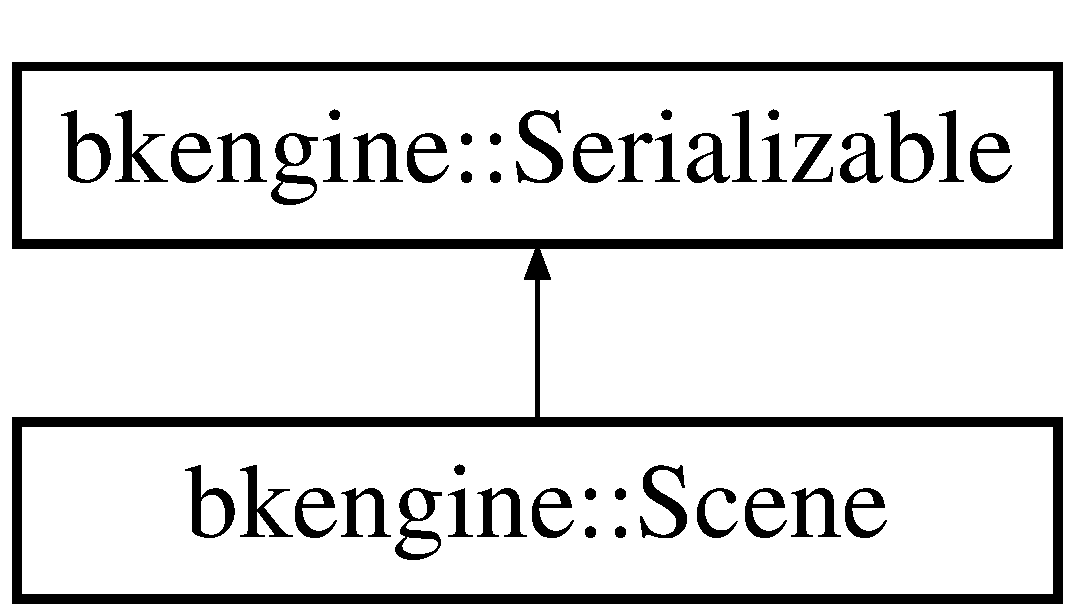
\includegraphics[height=2.000000cm]{classbkengine_1_1Scene}
\end{center}
\end{figure}
\subsection*{Public Member Functions}
\begin{DoxyCompactItemize}
\item 
\mbox{\Hypertarget{classbkengine_1_1Scene_a3127e57e1ff42edb9c3cda34d27249c2}\label{classbkengine_1_1Scene_a3127e57e1ff42edb9c3cda34d27249c2}} 
bool {\bfseries has\+Element} (const std\+::string \&name) const
\item 
\mbox{\Hypertarget{classbkengine_1_1Scene_afe21a71bdcef366a6e6be0779db675d7}\label{classbkengine_1_1Scene_afe21a71bdcef366a6e6be0779db675d7}} 
bool {\bfseries has\+Element} (unsigned int index) const
\item 
\mbox{\Hypertarget{classbkengine_1_1Scene_a6b9eddaef6e6f1e5845627a27f4c0855}\label{classbkengine_1_1Scene_a6b9eddaef6e6f1e5845627a27f4c0855}} 
void {\bfseries remove\+Element} (const std\+::string \&name)
\item 
\mbox{\Hypertarget{classbkengine_1_1Scene_a96c7a8bf8b818bb718a82410ed930997}\label{classbkengine_1_1Scene_a96c7a8bf8b818bb718a82410ed930997}} 
void {\bfseries remove\+Element} (unsigned int index)
\item 
\mbox{\Hypertarget{classbkengine_1_1Scene_a6bdf98fd9bef98e82744d92915651ec7}\label{classbkengine_1_1Scene_a6bdf98fd9bef98e82744d92915651ec7}} 
\hyperlink{classbkengine_1_1Element}{Element} \& {\bfseries get\+Element} (unsigned int index)
\item 
\mbox{\Hypertarget{classbkengine_1_1Scene_a9023f6c7dd5dd75ea1b0410265f06d5e}\label{classbkengine_1_1Scene_a9023f6c7dd5dd75ea1b0410265f06d5e}} 
\hyperlink{classbkengine_1_1Element}{Element} \& {\bfseries get\+Element} (const std\+::string \&name)
\item 
\mbox{\Hypertarget{classbkengine_1_1Scene_a2750a0b50166349395b8c0a31f34a414}\label{classbkengine_1_1Scene_a2750a0b50166349395b8c0a31f34a414}} 
{\footnotesize template$<$typename T $>$ }\\T \& {\bfseries add\+Element} (const T \&)
\item 
\mbox{\Hypertarget{classbkengine_1_1Scene_acbb42fedce808f75e0f82e59f3bfa43c}\label{classbkengine_1_1Scene_acbb42fedce808f75e0f82e59f3bfa43c}} 
{\footnotesize template$<$typename T $>$ }\\T \& {\bfseries add\+Element} (const std\+::shared\+\_\+ptr$<$ T $>$ \&)
\item 
\mbox{\Hypertarget{classbkengine_1_1Scene_af5481a1f876f29a0ef178e8fb583d0b2}\label{classbkengine_1_1Scene_af5481a1f876f29a0ef178e8fb583d0b2}} 
{\footnotesize template$<$typename T , typename... Params$>$ }\\T \& {\bfseries add\+Element} (Params...)
\item 
\mbox{\Hypertarget{classbkengine_1_1Scene_a3af9c0e5920908dc2b55c09f3ac63f05}\label{classbkengine_1_1Scene_a3af9c0e5920908dc2b55c09f3ac63f05}} 
{\footnotesize template$<$typename T $>$ }\\T \& {\bfseries get\+Element} (const std\+::string \&name)
\item 
\mbox{\Hypertarget{classbkengine_1_1Scene_afe0c7bb1ad5cfd3051d77e453275afbc}\label{classbkengine_1_1Scene_afe0c7bb1ad5cfd3051d77e453275afbc}} 
{\footnotesize template$<$typename T $>$ }\\T \& {\bfseries get\+Element} (unsigned int index)
\item 
\mbox{\Hypertarget{classbkengine_1_1Scene_ad38687f5ba8e021eae3be69d65eb8793}\label{classbkengine_1_1Scene_ad38687f5ba8e021eae3be69d65eb8793}} 
std\+::string {\bfseries get\+Name} () const
\item 
\mbox{\Hypertarget{classbkengine_1_1Scene_a5e0f80e658596a1b5641bdcadd748eb1}\label{classbkengine_1_1Scene_a5e0f80e658596a1b5641bdcadd748eb1}} 
{\bfseries Scene} (\hyperlink{classbkengine_1_1Game}{Game} $\ast$parent\+Game=nullptr, const std\+::string \&name=\char`\"{}\char`\"{})
\item 
\mbox{\Hypertarget{classbkengine_1_1Scene_a908f0ea17201652c169a1ccd2ed9e6c1}\label{classbkengine_1_1Scene_a908f0ea17201652c169a1ccd2ed9e6c1}} 
{\bfseries Scene} (\hyperlink{classbkengine_1_1Scene}{Scene} \&\&scene)
\item 
\mbox{\Hypertarget{classbkengine_1_1Scene_a85ff28a4e5b89c819cf145bcd6b2f96e}\label{classbkengine_1_1Scene_a85ff28a4e5b89c819cf145bcd6b2f96e}} 
\hyperlink{classbkengine_1_1Scene}{Scene} \& {\bfseries operator=} (\hyperlink{classbkengine_1_1Scene}{Scene} \&\&scene)
\item 
\mbox{\Hypertarget{classbkengine_1_1Scene_ac6e562fa1a4acfc552231f6dc31b6319}\label{classbkengine_1_1Scene_ac6e562fa1a4acfc552231f6dc31b6319}} 
virtual void {\bfseries setup\+Environment} ()
\item 
\mbox{\Hypertarget{classbkengine_1_1Scene_a59db4aed9b0a6c097c53f367a468a894}\label{classbkengine_1_1Scene_a59db4aed9b0a6c097c53f367a468a894}} 
virtual void {\bfseries setup\+Elements} ()
\item 
\mbox{\Hypertarget{classbkengine_1_1Scene_a2fbdf62053d4c57c27a1a73af8b1aad1}\label{classbkengine_1_1Scene_a2fbdf62053d4c57c27a1a73af8b1aad1}} 
virtual void {\bfseries on\+Loop} ()
\item 
\mbox{\Hypertarget{classbkengine_1_1Scene_afda94c0c7067d5f30b62f2850926876c}\label{classbkengine_1_1Scene_afda94c0c7067d5f30b62f2850926876c}} 
virtual void {\bfseries on\+Render} ()
\item 
\mbox{\Hypertarget{classbkengine_1_1Scene_ab397349c749fb47dae6fe40447c130dd}\label{classbkengine_1_1Scene_ab397349c749fb47dae6fe40447c130dd}} 
virtual bool {\bfseries on\+Event} (const \hyperlink{classbkengine_1_1Event}{Event} \&)
\item 
\mbox{\Hypertarget{classbkengine_1_1Scene_a70e5b1218abb729d70d9f41b107017f9}\label{classbkengine_1_1Scene_a70e5b1218abb729d70d9f41b107017f9}} 
void {\bfseries clear} ()
\item 
\mbox{\Hypertarget{classbkengine_1_1Scene_af4a628160b935f47a247c9abbe083598}\label{classbkengine_1_1Scene_af4a628160b935f47a247c9abbe083598}} 
virtual void {\bfseries deserialize} (const Json\+::\+Value \&) override
\item 
\mbox{\Hypertarget{classbkengine_1_1Scene_a14a8d5ffd84e2fe7babafaff7a39fd73}\label{classbkengine_1_1Scene_a14a8d5ffd84e2fe7babafaff7a39fd73}} 
virtual Json\+::\+Value {\bfseries serialize} () const override
\item 
\mbox{\Hypertarget{classbkengine_1_1Scene_a8b72aa22a98f75e49cef5eaa531e2d95}\label{classbkengine_1_1Scene_a8b72aa22a98f75e49cef5eaa531e2d95}} 
{\footnotesize template$<$typename T $>$ }\\T \& {\bfseries add\+Element} (const T \&element)
\item 
\mbox{\Hypertarget{classbkengine_1_1Scene_a14a6dc3997d94ecd1410fa2595ab3eb6}\label{classbkengine_1_1Scene_a14a6dc3997d94ecd1410fa2595ab3eb6}} 
{\footnotesize template$<$typename T $>$ }\\T \& {\bfseries add\+Element} (const std\+::shared\+\_\+ptr$<$ T $>$ \&element)
\item 
\mbox{\Hypertarget{classbkengine_1_1Scene_a5d54191111b9d4b1f6a95730c5affbb1}\label{classbkengine_1_1Scene_a5d54191111b9d4b1f6a95730c5affbb1}} 
{\footnotesize template$<$typename T , typename... Params$>$ }\\T \& {\bfseries add\+Element} (Params... params)
\item 
\mbox{\Hypertarget{classbkengine_1_1Scene_a1695992fd5f3340dc9c78d4bb64ad753}\label{classbkengine_1_1Scene_a1695992fd5f3340dc9c78d4bb64ad753}} 
{\footnotesize template$<$typename T $>$ }\\T \& {\bfseries get\+Element} (const std\+::string \&name)
\item 
\mbox{\Hypertarget{classbkengine_1_1Scene_a2004416cacbd5a6ae3dcd303609d640a}\label{classbkengine_1_1Scene_a2004416cacbd5a6ae3dcd303609d640a}} 
{\footnotesize template$<$typename T $>$ }\\T \& {\bfseries get\+Element} (unsigned int index)
\end{DoxyCompactItemize}
\subsection*{Friends}
\begin{DoxyCompactItemize}
\item 
\mbox{\Hypertarget{classbkengine_1_1Scene_a016b821f88c7c0a2de1451c175cefbf9}\label{classbkengine_1_1Scene_a016b821f88c7c0a2de1451c175cefbf9}} 
class {\bfseries Element}
\item 
\mbox{\Hypertarget{classbkengine_1_1Scene_aa2fab026580d6f14280c2ffb8063a314}\label{classbkengine_1_1Scene_aa2fab026580d6f14280c2ffb8063a314}} 
class {\bfseries Game}
\end{DoxyCompactItemize}


\subsection{Detailed Description}


Definition at line 15 of file Scene.\+h.



The documentation for this class was generated from the following files\+:\begin{DoxyCompactItemize}
\item 
/home/skaupper/dev/\+B\+K\+Engine/include/bkengine/Scene.\+h\item 
/home/skaupper/dev/\+B\+K\+Engine/include/bkengine/templates/Scene\+\_\+templates.\+h\item 
/home/skaupper/dev/\+B\+K\+Engine/src/Scene.\+cpp\end{DoxyCompactItemize}

\hypertarget{classbkengine_1_1SDLEventInterface}{}\section{bkengine\+:\+:S\+D\+L\+Event\+Interface Class Reference}
\label{classbkengine_1_1SDLEventInterface}\index{bkengine\+::\+S\+D\+L\+Event\+Interface@{bkengine\+::\+S\+D\+L\+Event\+Interface}}
Inheritance diagram for bkengine\+:\+:S\+D\+L\+Event\+Interface\+:\begin{figure}[H]
\begin{center}
\leavevmode
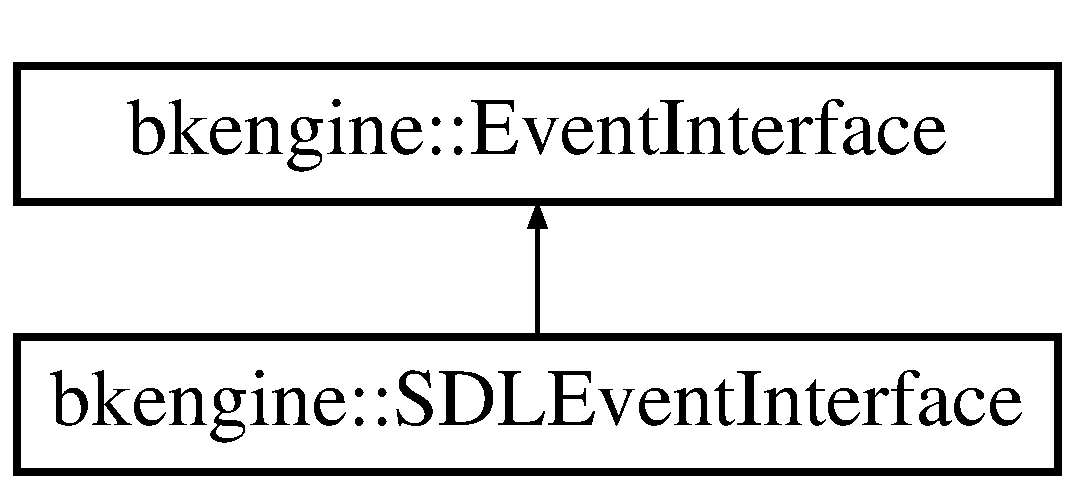
\includegraphics[height=2.000000cm]{classbkengine_1_1SDLEventInterface}
\end{center}
\end{figure}
\subsection*{Public Member Functions}
\begin{DoxyCompactItemize}
\item 
\mbox{\Hypertarget{classbkengine_1_1SDLEventInterface_a3ab921ee8788de5d7f9484d517088b29}\label{classbkengine_1_1SDLEventInterface_a3ab921ee8788de5d7f9484d517088b29}} 
virtual bool {\bfseries ready} ()
\item 
\mbox{\Hypertarget{classbkengine_1_1SDLEventInterface_a86d38142252d30b76aab60007569e7f1}\label{classbkengine_1_1SDLEventInterface_a86d38142252d30b76aab60007569e7f1}} 
virtual \hyperlink{classbkengine_1_1Event}{Event} {\bfseries poll} ()
\end{DoxyCompactItemize}


\subsection{Detailed Description}


Definition at line 12 of file S\+D\+L\+Event\+Interface.\+h.



The documentation for this class was generated from the following files\+:\begin{DoxyCompactItemize}
\item 
/home/skaupper/dev/\+B\+K\+Engine/include/bkengine/S\+D\+L\+Event\+Interface.\+h\item 
/home/skaupper/dev/\+B\+K\+Engine/src/S\+D\+L\+Event\+Interface.\+cpp\end{DoxyCompactItemize}

\hypertarget{classSDLMock}{}\section{S\+D\+L\+Mock Class Reference}
\label{classSDLMock}\index{S\+D\+L\+Mock@{S\+D\+L\+Mock}}
Inheritance diagram for S\+D\+L\+Mock\+:\begin{figure}[H]
\begin{center}
\leavevmode
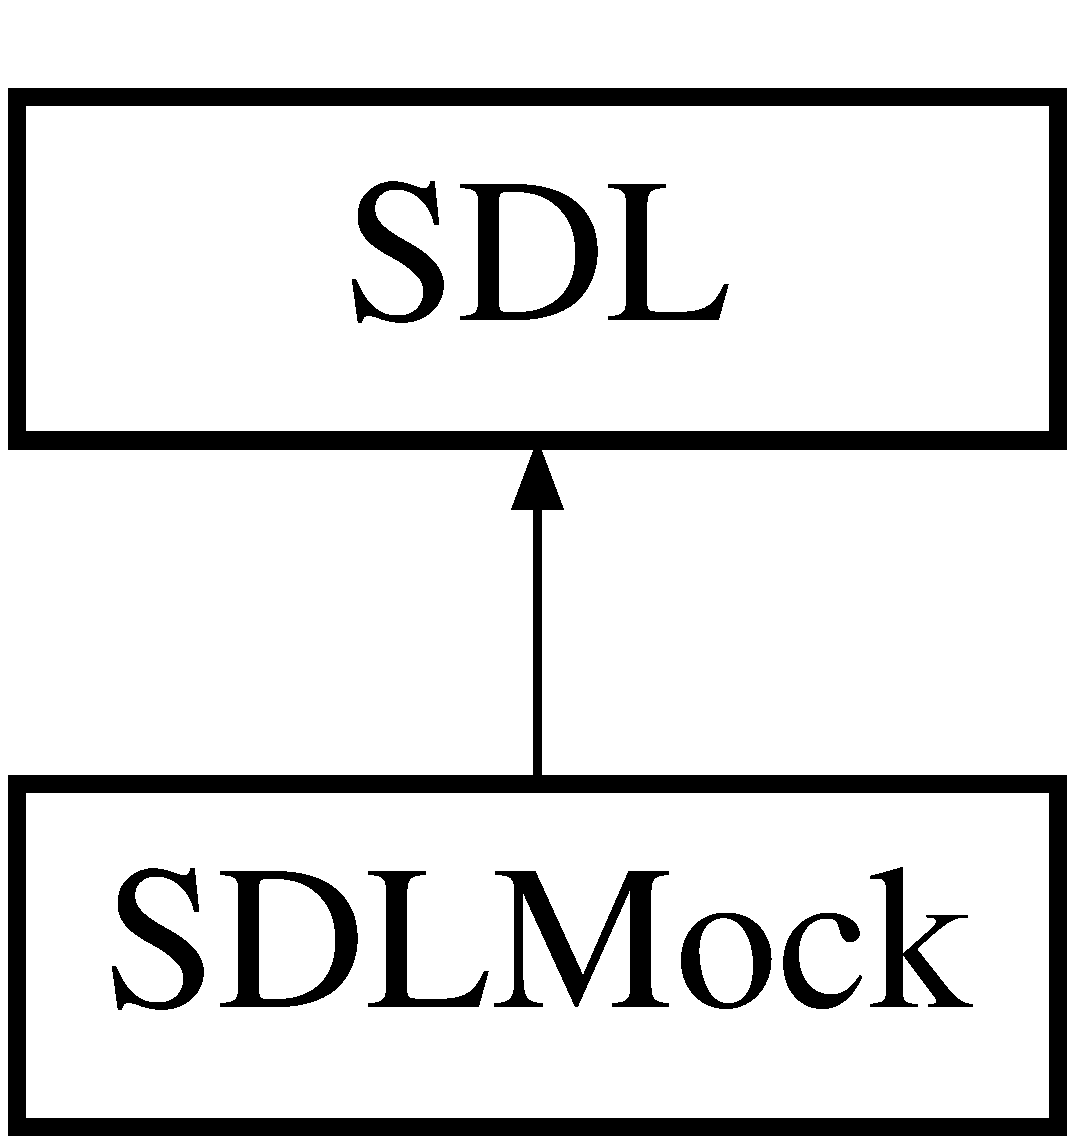
\includegraphics[height=2.000000cm]{classSDLMock}
\end{center}
\end{figure}
\subsection*{Public Member Functions}
\begin{DoxyCompactItemize}
\item 
\mbox{\Hypertarget{classSDLMock_a0922c5ef963abd254c463063b81a1407}\label{classSDLMock_a0922c5ef963abd254c463063b81a1407}} 
{\bfseries M\+O\+C\+K\+\_\+\+M\+E\+T\+H\+O\+D0} (S\+D\+L\+\_\+\+Get\+Error, const char $\ast$())
\item 
\mbox{\Hypertarget{classSDLMock_a8c253aa6691f49a181d589ce5d3cb141}\label{classSDLMock_a8c253aa6691f49a181d589ce5d3cb141}} 
{\bfseries M\+O\+C\+K\+\_\+\+M\+E\+T\+H\+O\+D1} (S\+D\+L\+\_\+\+Destroy\+Renderer, void(S\+D\+L\+\_\+\+Renderer $\ast$))
\item 
\mbox{\Hypertarget{classSDLMock_a1270866dc6be83a224a53734883fa60c}\label{classSDLMock_a1270866dc6be83a224a53734883fa60c}} 
{\bfseries M\+O\+C\+K\+\_\+\+M\+E\+T\+H\+O\+D1} (S\+D\+L\+\_\+\+Destroy\+Window, void(S\+D\+L\+\_\+\+Window $\ast$))
\item 
\mbox{\Hypertarget{classSDLMock_acb91d7819df1b2bc453173db9ed70389}\label{classSDLMock_acb91d7819df1b2bc453173db9ed70389}} 
{\bfseries M\+O\+C\+K\+\_\+\+M\+E\+T\+H\+O\+D0} (S\+D\+L\+\_\+\+Quit, void())
\item 
\mbox{\Hypertarget{classSDLMock_aa555627d7f34fb08a442aab406a5619c}\label{classSDLMock_aa555627d7f34fb08a442aab406a5619c}} 
{\bfseries M\+O\+C\+K\+\_\+\+M\+E\+T\+H\+O\+D1} (S\+D\+L\+\_\+\+Init, int(uint32\+\_\+t))
\item 
\mbox{\Hypertarget{classSDLMock_ad846bdb6738a4e9daeffaf118b78fd78}\label{classSDLMock_ad846bdb6738a4e9daeffaf118b78fd78}} 
{\bfseries M\+O\+C\+K\+\_\+\+M\+E\+T\+H\+O\+D2} (S\+D\+L\+\_\+\+Set\+Hint, S\+D\+L\+\_\+bool(const char $\ast$, const char $\ast$))
\item 
\mbox{\Hypertarget{classSDLMock_ab1f3a182c097e7f56e622cb9a475669e}\label{classSDLMock_ab1f3a182c097e7f56e622cb9a475669e}} 
{\bfseries M\+O\+C\+K\+\_\+\+M\+E\+T\+H\+O\+D6} (S\+D\+L\+\_\+\+Create\+Window, S\+D\+L\+\_\+\+Window $\ast$(const char $\ast$, int, int, int, int, uint32\+\_\+t))
\item 
\mbox{\Hypertarget{classSDLMock_a8d6247ca471a04b9a63e8121bcbca7ff}\label{classSDLMock_a8d6247ca471a04b9a63e8121bcbca7ff}} 
{\bfseries M\+O\+C\+K\+\_\+\+M\+E\+T\+H\+O\+D2} (S\+D\+L\+\_\+\+Set\+Window\+Icon, void(S\+D\+L\+\_\+\+Window $\ast$, S\+D\+L\+\_\+\+Surface $\ast$))
\item 
\mbox{\Hypertarget{classSDLMock_a658576368c9a958936a638bd91453ea5}\label{classSDLMock_a658576368c9a958936a638bd91453ea5}} 
{\bfseries M\+O\+C\+K\+\_\+\+M\+E\+T\+H\+O\+D1} (S\+D\+L\+\_\+\+Free\+Surface, void(S\+D\+L\+\_\+\+Surface $\ast$))
\item 
\mbox{\Hypertarget{classSDLMock_aaff62f5c69eeb30fcb0cdb7415163d80}\label{classSDLMock_aaff62f5c69eeb30fcb0cdb7415163d80}} 
{\bfseries M\+O\+C\+K\+\_\+\+M\+E\+T\+H\+O\+D3} (S\+D\+L\+\_\+\+Create\+Renderer, S\+D\+L\+\_\+\+Renderer $\ast$(S\+D\+L\+\_\+\+Window $\ast$, int, uint32\+\_\+t))
\item 
\mbox{\Hypertarget{classSDLMock_aa4bba6254b823069672361b6c5a95ff2}\label{classSDLMock_aa4bba6254b823069672361b6c5a95ff2}} 
{\bfseries M\+O\+C\+K\+\_\+\+M\+E\+T\+H\+O\+D5} (S\+D\+L\+\_\+\+Set\+Render\+Draw\+Color, int(S\+D\+L\+\_\+\+Renderer $\ast$, uint8\+\_\+t, uint8\+\_\+t, uint8\+\_\+t, uint8\+\_\+t))
\item 
\mbox{\Hypertarget{classSDLMock_a7c65e1143e4e8bc1637e25c3cc37357e}\label{classSDLMock_a7c65e1143e4e8bc1637e25c3cc37357e}} 
{\bfseries M\+O\+C\+K\+\_\+\+M\+E\+T\+H\+O\+D1} (S\+D\+L\+\_\+\+Poll\+Event, int(S\+D\+L\+\_\+\+Event $\ast$))
\item 
\mbox{\Hypertarget{classSDLMock_a2c4e72a0b0158285c2bfb1eaec1cbb12}\label{classSDLMock_a2c4e72a0b0158285c2bfb1eaec1cbb12}} 
{\bfseries M\+O\+C\+K\+\_\+\+M\+E\+T\+H\+O\+D1} (S\+D\+L\+\_\+\+Delay, void(uint32\+\_\+t))
\item 
\mbox{\Hypertarget{classSDLMock_a20f0745fa1567a29273045ef430c8b22}\label{classSDLMock_a20f0745fa1567a29273045ef430c8b22}} 
{\bfseries M\+O\+C\+K\+\_\+\+M\+E\+T\+H\+O\+D1} (S\+D\+L\+\_\+\+Render\+Clear, int(S\+D\+L\+\_\+\+Renderer $\ast$))
\item 
\mbox{\Hypertarget{classSDLMock_aabda25c5efe41cc214ffcbfba4f03ffc}\label{classSDLMock_aabda25c5efe41cc214ffcbfba4f03ffc}} 
{\bfseries M\+O\+C\+K\+\_\+\+M\+E\+T\+H\+O\+D1} (S\+D\+L\+\_\+\+Render\+Present, void(S\+D\+L\+\_\+\+Renderer $\ast$))
\item 
\mbox{\Hypertarget{classSDLMock_ac25fb9830d2e388f4e681d53fc51dce9}\label{classSDLMock_ac25fb9830d2e388f4e681d53fc51dce9}} 
{\bfseries M\+O\+C\+K\+\_\+\+M\+E\+T\+H\+O\+D1} (S\+D\+L\+\_\+\+Destroy\+Texture, void(S\+D\+L\+\_\+\+Texture $\ast$))
\item 
\mbox{\Hypertarget{classSDLMock_acc8333f8abbe99a67a13cefeecaefb32}\label{classSDLMock_acc8333f8abbe99a67a13cefeecaefb32}} 
{\bfseries M\+O\+C\+K\+\_\+\+M\+E\+T\+H\+O\+D2} (S\+D\+L\+\_\+\+Create\+Texture\+From\+Surface, S\+D\+L\+\_\+\+Texture $\ast$(S\+D\+L\+\_\+\+Renderer $\ast$, S\+D\+L\+\_\+\+Surface $\ast$))
\item 
\mbox{\Hypertarget{classSDLMock_adef6a49962945e23cc287caccc3a84e8}\label{classSDLMock_adef6a49962945e23cc287caccc3a84e8}} 
{\bfseries M\+O\+C\+K\+\_\+\+M\+E\+T\+H\+O\+D5} (S\+D\+L\+\_\+\+Query\+Texture, int(S\+D\+L\+\_\+\+Texture $\ast$, uint32\+\_\+t $\ast$, int $\ast$, int $\ast$, int $\ast$))
\item 
\mbox{\Hypertarget{classSDLMock_aaa0d5ea9ea703f31eebb2a18bf119828}\label{classSDLMock_aaa0d5ea9ea703f31eebb2a18bf119828}} 
{\bfseries M\+O\+C\+K\+\_\+\+M\+E\+T\+H\+O\+D3} (S\+D\+L\+\_\+\+Get\+Window\+Size, void(S\+D\+L\+\_\+\+Window $\ast$, int $\ast$, int $\ast$))
\item 
\mbox{\Hypertarget{classSDLMock_a4e3accd6fba192ed90c06729ce3fa566}\label{classSDLMock_a4e3accd6fba192ed90c06729ce3fa566}} 
{\bfseries M\+O\+C\+K\+\_\+\+M\+E\+T\+H\+O\+D1} (S\+D\+L\+\_\+\+Get\+Window\+Title, const char $\ast$(S\+D\+L\+\_\+\+Window $\ast$))
\item 
\mbox{\Hypertarget{classSDLMock_afdff18b55ec4e6b488db8440581b9d20}\label{classSDLMock_afdff18b55ec4e6b488db8440581b9d20}} 
{\bfseries M\+O\+C\+K\+\_\+\+M\+E\+T\+H\+O\+D7} (S\+D\+L\+\_\+\+Render\+Copy\+Ex, int(S\+D\+L\+\_\+\+Renderer $\ast$, S\+D\+L\+\_\+\+Texture $\ast$, const S\+D\+L\+\_\+\+Rect $\ast$, const S\+D\+L\+\_\+\+Rect $\ast$, const double, const S\+D\+L\+\_\+\+Point $\ast$, const S\+D\+L\+\_\+\+Renderer\+Flip))
\item 
\mbox{\Hypertarget{classSDLMock_a0494f469f47cb2f5591dc22d400aca08}\label{classSDLMock_a0494f469f47cb2f5591dc22d400aca08}} 
{\bfseries M\+O\+C\+K\+\_\+\+M\+E\+T\+H\+O\+D4} (S\+D\+L\+\_\+\+Render\+Copy, int(S\+D\+L\+\_\+\+Renderer $\ast$, S\+D\+L\+\_\+\+Texture $\ast$, const S\+D\+L\+\_\+\+Rect $\ast$, const S\+D\+L\+\_\+\+Rect $\ast$))
\item 
\mbox{\Hypertarget{classSDLMock_abe4a22b5adce6b21b9dd81c7929ebff7}\label{classSDLMock_abe4a22b5adce6b21b9dd81c7929ebff7}} 
{\bfseries M\+O\+C\+K\+\_\+\+M\+E\+T\+H\+O\+D0} (S\+D\+L\+\_\+\+Get\+Ticks, uint32\+\_\+t())
\item 
\mbox{\Hypertarget{classSDLMock_a7d11b0bd17dd806269d1a6d118687fbb}\label{classSDLMock_a7d11b0bd17dd806269d1a6d118687fbb}} 
{\bfseries M\+O\+C\+K\+\_\+\+M\+E\+T\+H\+O\+D0} (T\+T\+F\+\_\+\+Init, int())
\item 
\mbox{\Hypertarget{classSDLMock_aa451d78bba36016af9c89ed21b757aed}\label{classSDLMock_aa451d78bba36016af9c89ed21b757aed}} 
{\bfseries M\+O\+C\+K\+\_\+\+M\+E\+T\+H\+O\+D2} (T\+T\+F\+\_\+\+Open\+Font, T\+T\+F\+\_\+\+Font $\ast$(const char $\ast$, int))
\item 
\mbox{\Hypertarget{classSDLMock_a167f794e4df063476013a91307afdbe1}\label{classSDLMock_a167f794e4df063476013a91307afdbe1}} 
{\bfseries M\+O\+C\+K\+\_\+\+M\+E\+T\+H\+O\+D3} (T\+T\+F\+\_\+\+Render\+Text\+\_\+\+Solid, S\+D\+L\+\_\+\+Surface $\ast$(T\+T\+F\+\_\+\+Font $\ast$, const char $\ast$, S\+D\+L\+\_\+\+Color))
\item 
\mbox{\Hypertarget{classSDLMock_a22f101992bbdbd9130b32a357e07906d}\label{classSDLMock_a22f101992bbdbd9130b32a357e07906d}} 
{\bfseries M\+O\+C\+K\+\_\+\+M\+E\+T\+H\+O\+D1} (T\+T\+F\+\_\+\+Close\+Font, void(T\+T\+F\+\_\+\+Font $\ast$))
\item 
\mbox{\Hypertarget{classSDLMock_acaace20d5e817097c3edbc5c1a4b1f3d}\label{classSDLMock_acaace20d5e817097c3edbc5c1a4b1f3d}} 
{\bfseries M\+O\+C\+K\+\_\+\+M\+E\+T\+H\+O\+D0} (T\+T\+F\+\_\+\+Quit, void())
\item 
\mbox{\Hypertarget{classSDLMock_ae75ec568e235fa9757a16f04bc21362c}\label{classSDLMock_ae75ec568e235fa9757a16f04bc21362c}} 
{\bfseries M\+O\+C\+K\+\_\+\+M\+E\+T\+H\+O\+D1} (I\+M\+G\+\_\+\+Init, int(int))
\item 
\mbox{\Hypertarget{classSDLMock_ab2c158ba13a0d6d7940952b8035c6a63}\label{classSDLMock_ab2c158ba13a0d6d7940952b8035c6a63}} 
{\bfseries M\+O\+C\+K\+\_\+\+M\+E\+T\+H\+O\+D1} (I\+M\+G\+\_\+\+Load, S\+D\+L\+\_\+\+Surface $\ast$(const char $\ast$))
\item 
\mbox{\Hypertarget{classSDLMock_a634219e9f1b4a82d0c281377c6bc06c7}\label{classSDLMock_a634219e9f1b4a82d0c281377c6bc06c7}} 
{\bfseries M\+O\+C\+K\+\_\+\+M\+E\+T\+H\+O\+D0} (I\+M\+G\+\_\+\+Quit, void())
\item 
\mbox{\Hypertarget{classSDLMock_a93c15996fd5209123c253b1747751a8b}\label{classSDLMock_a93c15996fd5209123c253b1747751a8b}} 
{\bfseries M\+O\+C\+K\+\_\+\+M\+E\+T\+H\+O\+D4} (Mix\+\_\+\+Open\+Audio, int(int, uint16\+\_\+t, int, int))
\item 
\mbox{\Hypertarget{classSDLMock_a7d12dc6f716e903b1a4a45ddbf22497c}\label{classSDLMock_a7d12dc6f716e903b1a4a45ddbf22497c}} 
{\bfseries M\+O\+C\+K\+\_\+\+M\+E\+T\+H\+O\+D0} (Mix\+\_\+\+Quit, void())
\end{DoxyCompactItemize}


\subsection{Detailed Description}


Definition at line 10 of file S\+D\+L\+Mock.\+h.



The documentation for this class was generated from the following file\+:\begin{DoxyCompactItemize}
\item 
/home/skaupper/dev/\+B\+K\+Engine/tests/S\+D\+L\+Mock.\+h\end{DoxyCompactItemize}

\hypertarget{classbkengine_1_1Serializable}{}\section{bkengine\+:\+:Serializable Class Reference}
\label{classbkengine_1_1Serializable}\index{bkengine\+::\+Serializable@{bkengine\+::\+Serializable}}
Inheritance diagram for bkengine\+:\+:Serializable\+:\begin{figure}[H]
\begin{center}
\leavevmode
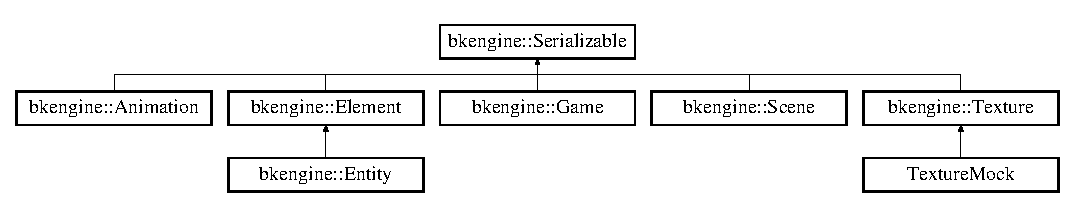
\includegraphics[height=2.349650cm]{classbkengine_1_1Serializable}
\end{center}
\end{figure}
\subsection*{Public Member Functions}
\begin{DoxyCompactItemize}
\item 
\mbox{\Hypertarget{classbkengine_1_1Serializable_adcb6ba349430cf279d985a31c9251d1f}\label{classbkengine_1_1Serializable_adcb6ba349430cf279d985a31c9251d1f}} 
virtual void {\bfseries deserialize} (const Json\+::\+Value \&)
\item 
\mbox{\Hypertarget{classbkengine_1_1Serializable_a44d249742000d1818b44bde3ebcfe3ce}\label{classbkengine_1_1Serializable_a44d249742000d1818b44bde3ebcfe3ce}} 
virtual Json\+::\+Value {\bfseries serialize} () const =0
\item 
\mbox{\Hypertarget{classbkengine_1_1Serializable_ad97f199bcd3cfe35b1e29adead7acf74}\label{classbkengine_1_1Serializable_ad97f199bcd3cfe35b1e29adead7acf74}} 
void {\bfseries set} ()
\item 
\mbox{\Hypertarget{classbkengine_1_1Serializable_a283a95509d8ab2e8cb6d0ac4b8d2d8d9}\label{classbkengine_1_1Serializable_a283a95509d8ab2e8cb6d0ac4b8d2d8d9}} 
void {\bfseries reset} ()
\item 
\mbox{\Hypertarget{classbkengine_1_1Serializable_a72754434ccc30248fc64faaca277c69b}\label{classbkengine_1_1Serializable_a72754434ccc30248fc64faaca277c69b}} 
std\+::string {\bfseries to\+String} () const
\end{DoxyCompactItemize}


\subsection{Detailed Description}


Definition at line 13 of file Serializable.\+h.



The documentation for this class was generated from the following files\+:\begin{DoxyCompactItemize}
\item 
/home/skaupper/dev/\+B\+K\+Engine/include/bkengine/Serializable.\+h\item 
/home/skaupper/dev/\+B\+K\+Engine/src/Serializable.\+cpp\end{DoxyCompactItemize}

\hypertarget{classbkengine_1_1Serializer}{}\section{bkengine\+:\+:Serializer Class Reference}
\label{classbkengine_1_1Serializer}\index{bkengine\+::\+Serializer@{bkengine\+::\+Serializer}}
\subsection*{Static Public Member Functions}
\begin{DoxyCompactItemize}
\item 
\mbox{\Hypertarget{classbkengine_1_1Serializer_a80fab1c59d2ddbb9328f6428fb404a66}\label{classbkengine_1_1Serializer_a80fab1c59d2ddbb9328f6428fb404a66}} 
{\footnotesize template$<$typename T $>$ }\\static void {\bfseries add\+Type} (const std\+::string \&name)
\item 
\mbox{\Hypertarget{classbkengine_1_1Serializer_ac41e89308a3a250d3fcc2c6ded2fd468}\label{classbkengine_1_1Serializer_ac41e89308a3a250d3fcc2c6ded2fd468}} 
{\footnotesize template$<$typename T $>$ }\\static std\+::shared\+\_\+ptr$<$ T $>$ {\bfseries get\+Instance} (const std\+::string \&name)
\end{DoxyCompactItemize}


\subsection{Detailed Description}


Definition at line 30 of file Serializable.\+h.



The documentation for this class was generated from the following files\+:\begin{DoxyCompactItemize}
\item 
/home/skaupper/dev/\+B\+K\+Engine/include/bkengine/Serializable.\+h\item 
/home/skaupper/dev/\+B\+K\+Engine/src/Serializable.\+cpp\end{DoxyCompactItemize}

\hypertarget{classbkengine_1_1SettingsInterface}{}\section{bkengine\+:\+:Settings\+Interface Class Reference}
\label{classbkengine_1_1SettingsInterface}\index{bkengine\+::\+Settings\+Interface@{bkengine\+::\+Settings\+Interface}}
Inheritance diagram for bkengine\+:\+:Settings\+Interface\+:\begin{figure}[H]
\begin{center}
\leavevmode
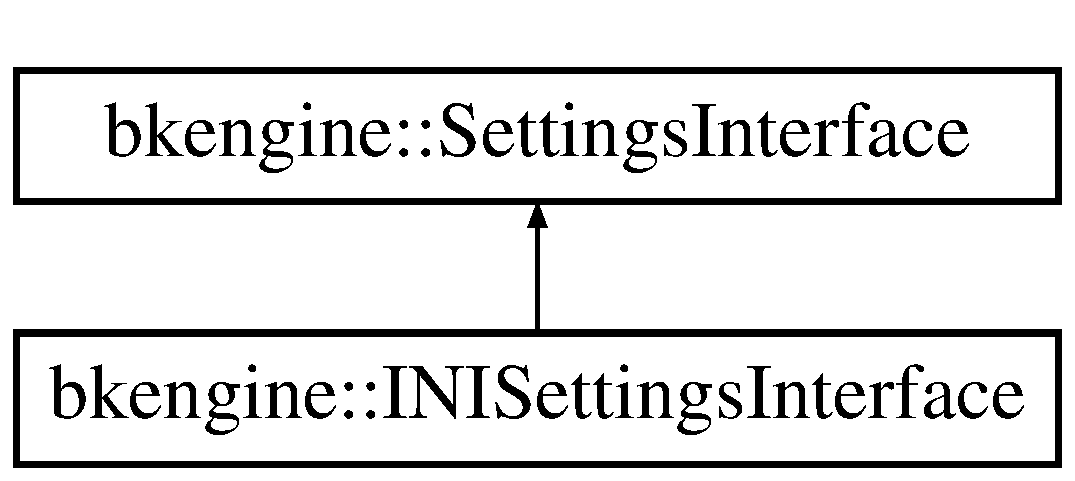
\includegraphics[height=2.000000cm]{classbkengine_1_1SettingsInterface}
\end{center}
\end{figure}
\subsection*{Public Member Functions}
\begin{DoxyCompactItemize}
\item 
\mbox{\Hypertarget{classbkengine_1_1SettingsInterface_a1022cfb0b4e25bc73563082456db3913}\label{classbkengine_1_1SettingsInterface_a1022cfb0b4e25bc73563082456db3913}} 
virtual void {\bfseries init} ()=0
\item 
\mbox{\Hypertarget{classbkengine_1_1SettingsInterface_a7f5937eb93d953422c997b00f6ba21a8}\label{classbkengine_1_1SettingsInterface_a7f5937eb93d953422c997b00f6ba21a8}} 
virtual void {\bfseries load\+From\+File} (const std\+::string \&filename)=0
\item 
\mbox{\Hypertarget{classbkengine_1_1SettingsInterface_a5aaaa97c4131306a4bd5b4635b08fd48}\label{classbkengine_1_1SettingsInterface_a5aaaa97c4131306a4bd5b4635b08fd48}} 
virtual void {\bfseries save\+To\+File} (const std\+::string \&filename) const =0
\item 
\mbox{\Hypertarget{classbkengine_1_1SettingsInterface_a8e8ab86b2ece557d6e54fe1bc5bcef49}\label{classbkengine_1_1SettingsInterface_a8e8ab86b2ece557d6e54fe1bc5bcef49}} 
virtual bool {\bfseries has\+Value} (const std\+::string \&key) const =0
\item 
\mbox{\Hypertarget{classbkengine_1_1SettingsInterface_a97607df1c2261e5311084283fdcb179e}\label{classbkengine_1_1SettingsInterface_a97607df1c2261e5311084283fdcb179e}} 
virtual std\+::string {\bfseries get} (const std\+::string \&key) const =0
\item 
\mbox{\Hypertarget{classbkengine_1_1SettingsInterface_a6d39b7291fe754dc1b24cb78078c29f8}\label{classbkengine_1_1SettingsInterface_a6d39b7291fe754dc1b24cb78078c29f8}} 
virtual std\+::string {\bfseries remove} (const std\+::string \&key)=0
\item 
\mbox{\Hypertarget{classbkengine_1_1SettingsInterface_a80131ee581fd983125b7c1b73152db8b}\label{classbkengine_1_1SettingsInterface_a80131ee581fd983125b7c1b73152db8b}} 
virtual void {\bfseries create} (const std\+::string \&key, const std\+::string \&value)=0
\item 
\mbox{\Hypertarget{classbkengine_1_1SettingsInterface_a596ab8a979efb83a290199aad8d445d7}\label{classbkengine_1_1SettingsInterface_a596ab8a979efb83a290199aad8d445d7}} 
virtual void {\bfseries change} (const std\+::string \&key, const std\+::string \&newvalue)=0
\item 
\mbox{\Hypertarget{classbkengine_1_1SettingsInterface_a69a7a944749bfe0319125e1ce416579c}\label{classbkengine_1_1SettingsInterface_a69a7a944749bfe0319125e1ce416579c}} 
virtual uint32\+\_\+t {\bfseries count} () const =0
\end{DoxyCompactItemize}


\subsection{Detailed Description}


Definition at line 9 of file Settings\+Interface.\+h.



The documentation for this class was generated from the following file\+:\begin{DoxyCompactItemize}
\item 
/home/skaupper/dev/\+B\+K\+Engine/include/bkengine/Settings\+Interface.\+h\end{DoxyCompactItemize}

\hypertarget{structbkengine_1_1Size}{}\section{bkengine\+:\+:Size Struct Reference}
\label{structbkengine_1_1Size}\index{bkengine\+::\+Size@{bkengine\+::\+Size}}
\subsection*{Public Member Functions}
\begin{DoxyCompactItemize}
\item 
\mbox{\Hypertarget{structbkengine_1_1Size_a83fc60222fdc4509baacd931f1f2e19f}\label{structbkengine_1_1Size_a83fc60222fdc4509baacd931f1f2e19f}} 
{\bfseries Size} (float w, float h)
\item 
\mbox{\Hypertarget{structbkengine_1_1Size_a20d8b4e9f54a2d32f46f4a0bc9fb8bf5}\label{structbkengine_1_1Size_a20d8b4e9f54a2d32f46f4a0bc9fb8bf5}} 
std\+::string {\bfseries to\+String} () const
\item 
\mbox{\Hypertarget{structbkengine_1_1Size_a855276eef78ff8379cdc357c0f2b35ce}\label{structbkengine_1_1Size_a855276eef78ff8379cdc357c0f2b35ce}} 
S\+D\+L\+\_\+\+Point {\bfseries to\+S\+D\+L\+Point} () const
\end{DoxyCompactItemize}
\subsection*{Public Attributes}
\begin{DoxyCompactItemize}
\item 
\mbox{\Hypertarget{structbkengine_1_1Size_a14fb3163bebe1c3f68a3c65c72673230}\label{structbkengine_1_1Size_a14fb3163bebe1c3f68a3c65c72673230}} 
float {\bfseries w}
\item 
\mbox{\Hypertarget{structbkengine_1_1Size_acbdb27a32a6c880a071a427892e582d2}\label{structbkengine_1_1Size_acbdb27a32a6c880a071a427892e582d2}} 
float {\bfseries h}
\end{DoxyCompactItemize}


\subsection{Detailed Description}


Definition at line 29 of file Misc.\+h.



The documentation for this struct was generated from the following files\+:\begin{DoxyCompactItemize}
\item 
/home/skaupper/dev/\+B\+K\+Engine/include/bkengine/Misc.\+h\item 
/home/skaupper/dev/\+B\+K\+Engine/src/Misc.\+cpp\end{DoxyCompactItemize}

\hypertarget{classbkengine_1_1Storage}{}\section{bkengine\+:\+:Storage Class Reference}
\label{classbkengine_1_1Storage}\index{bkengine\+::\+Storage@{bkengine\+::\+Storage}}
\subsection*{Public Member Functions}
\begin{DoxyCompactItemize}
\item 
\mbox{\Hypertarget{classbkengine_1_1Storage_aabb685ee2db8aea1090f0b88aff3c8bb}\label{classbkengine_1_1Storage_aabb685ee2db8aea1090f0b88aff3c8bb}} 
{\bfseries Storage} (const std\+::string \&type)
\item 
\mbox{\Hypertarget{classbkengine_1_1Storage_afa7bcd7e54058dddde2407ffff451436}\label{classbkengine_1_1Storage_afa7bcd7e54058dddde2407ffff451436}} 
const std\+::string \& {\bfseries get\+Type} () const
\end{DoxyCompactItemize}
\subsection*{Static Public Attributes}
\begin{DoxyCompactItemize}
\item 
\mbox{\Hypertarget{classbkengine_1_1Storage_a92b3d2d6295531b85638cfdb6d1b55b4}\label{classbkengine_1_1Storage_a92b3d2d6295531b85638cfdb6d1b55b4}} 
static const std\+::string {\bfseries T\+Y\+PE} = \char`\"{}S\+T\+O\+R\+A\+GE\char`\"{}
\end{DoxyCompactItemize}


\subsection{Detailed Description}


Definition at line 8 of file Storage.\+h.



The documentation for this class was generated from the following files\+:\begin{DoxyCompactItemize}
\item 
/home/skaupper/dev/\+B\+K\+Engine/include/bkengine/Storage.\+h\item 
/home/skaupper/dev/\+B\+K\+Engine/src/Storage.\+cpp\end{DoxyCompactItemize}

\hypertarget{classbkengine_1_1Texture}{}\section{bkengine\+:\+:Texture Class Reference}
\label{classbkengine_1_1Texture}\index{bkengine\+::\+Texture@{bkengine\+::\+Texture}}
Inheritance diagram for bkengine\+:\+:Texture\+:\begin{figure}[H]
\begin{center}
\leavevmode
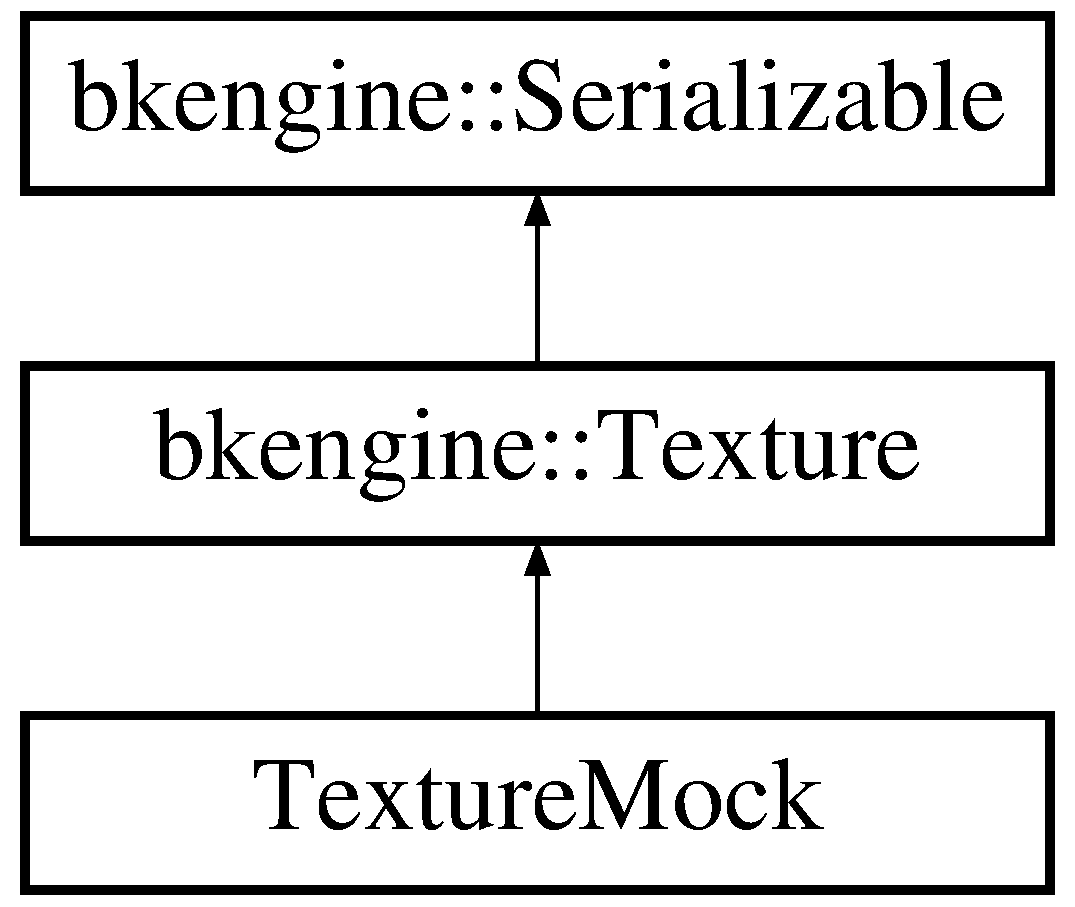
\includegraphics[height=3.000000cm]{classbkengine_1_1Texture}
\end{center}
\end{figure}
\subsection*{Public Member Functions}
\begin{DoxyCompactItemize}
\item 
\mbox{\Hypertarget{classbkengine_1_1Texture_aabea3eecbe16a0e44a280ed2ec1edb45}\label{classbkengine_1_1Texture_aabea3eecbe16a0e44a280ed2ec1edb45}} 
\hyperlink{structbkengine_1_1Rect}{Rect} {\bfseries get\+Size} () const
\item 
\mbox{\Hypertarget{classbkengine_1_1Texture_a68e73d6b3c30050ef410240b2de32fea}\label{classbkengine_1_1Texture_a68e73d6b3c30050ef410240b2de32fea}} 
void {\bfseries set\+Size} (int w, int h)
\item 
\mbox{\Hypertarget{classbkengine_1_1Texture_ad98c098ac51603405b2e8cb3237b5763}\label{classbkengine_1_1Texture_ad98c098ac51603405b2e8cb3237b5763}} 
void {\bfseries set\+Size} (const \hyperlink{structbkengine_1_1Rect}{Rect} \&rect)
\item 
\mbox{\Hypertarget{classbkengine_1_1Texture_a8b423c07980bfa1dbc54322bb6a65fbd}\label{classbkengine_1_1Texture_a8b423c07980bfa1dbc54322bb6a65fbd}} 
{\bfseries Texture} (const std\+::string \&font\+Name, const std\+::string \&text, const \hyperlink{structbkengine_1_1Rect}{Rect} \&size, const \hyperlink{structbkengine_1_1Color}{Color} \&color=\hyperlink{structbkengine_1_1Color}{Color}(), Text\+Quality quality=Text\+Quality\+::\+S\+O\+L\+ID)
\item 
\mbox{\Hypertarget{classbkengine_1_1Texture_a582d3c6b791a0da39cf5956fafa81801}\label{classbkengine_1_1Texture_a582d3c6b791a0da39cf5956fafa81801}} 
{\bfseries Texture} (const std\+::string \&path, const \hyperlink{structbkengine_1_1Rect}{Rect} \&size=\hyperlink{structbkengine_1_1Rect}{Rect}(), const \hyperlink{structbkengine_1_1Rect}{Rect} \&clip=\hyperlink{structbkengine_1_1Rect}{Rect}())
\item 
\mbox{\Hypertarget{classbkengine_1_1Texture_a3e67decde84b36228e612bd4a9f0a19c}\label{classbkengine_1_1Texture_a3e67decde84b36228e612bd4a9f0a19c}} 
virtual bool {\bfseries load\+Text} (const std\+::string \&font\+Name, const std\+::string \&text, const \hyperlink{structbkengine_1_1Rect}{Rect} \&size, const \hyperlink{structbkengine_1_1Color}{Color} \&color=\hyperlink{structbkengine_1_1Color}{Color}(), Text\+Quality quality=Text\+Quality\+::\+S\+O\+L\+ID)
\item 
\mbox{\Hypertarget{classbkengine_1_1Texture_a880fcd8dda876cb2c16390f079d8b99a}\label{classbkengine_1_1Texture_a880fcd8dda876cb2c16390f079d8b99a}} 
virtual bool {\bfseries load\+Image} (const std\+::string \&path, const \hyperlink{structbkengine_1_1Rect}{Rect} \&clip=\hyperlink{structbkengine_1_1Rect}{Rect}(), const \hyperlink{structbkengine_1_1Rect}{Rect} \&size=\hyperlink{structbkengine_1_1Rect}{Rect}())
\item 
\mbox{\Hypertarget{classbkengine_1_1Texture_a6a747f0cbe6320bd0e1a7f33281f0f7d}\label{classbkengine_1_1Texture_a6a747f0cbe6320bd0e1a7f33281f0f7d}} 
virtual void {\bfseries on\+Render} (const \hyperlink{structbkengine_1_1Rect}{Rect} \&parent\+Rect=\hyperlink{structbkengine_1_1Rect}{Rect}(), bool flip=false)
\item 
\mbox{\Hypertarget{classbkengine_1_1Texture_afaf8154bb525d6b600c1850822714d5c}\label{classbkengine_1_1Texture_afaf8154bb525d6b600c1850822714d5c}} 
virtual void {\bfseries deserialize} (const Json\+::\+Value \&) override
\item 
\mbox{\Hypertarget{classbkengine_1_1Texture_af1e8d8e6738ead367fadd06522be2c56}\label{classbkengine_1_1Texture_af1e8d8e6738ead367fadd06522be2c56}} 
virtual Json\+::\+Value {\bfseries serialize} () const override
\end{DoxyCompactItemize}


\subsection{Detailed Description}


Definition at line 20 of file Texture.\+h.



The documentation for this class was generated from the following files\+:\begin{DoxyCompactItemize}
\item 
/home/skaupper/dev/\+B\+K\+Engine/include/bkengine/Texture.\+h\item 
/home/skaupper/dev/\+B\+K\+Engine/src/Texture.\+cpp\end{DoxyCompactItemize}

\hypertarget{classTextureMock}{}\section{Texture\+Mock Class Reference}
\label{classTextureMock}\index{Texture\+Mock@{Texture\+Mock}}
Inheritance diagram for Texture\+Mock\+:\begin{figure}[H]
\begin{center}
\leavevmode
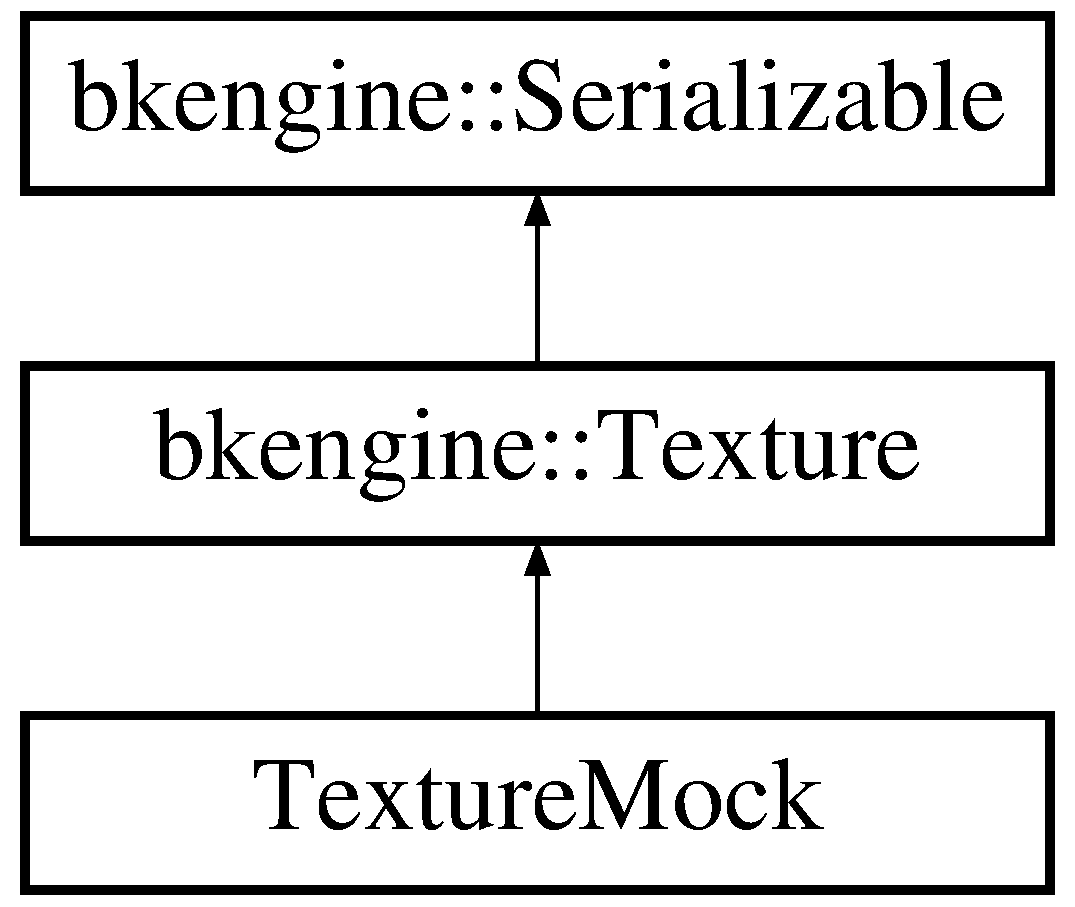
\includegraphics[height=3.000000cm]{classTextureMock}
\end{center}
\end{figure}
\subsection*{Static Public Attributes}
\begin{DoxyCompactItemize}
\item 
\mbox{\Hypertarget{classTextureMock_a7270b7f066e9f909afe0cf1f9e246fa5}\label{classTextureMock_a7270b7f066e9f909afe0cf1f9e246fa5}} 
static int {\bfseries init\+Count} = 0
\item 
\mbox{\Hypertarget{classTextureMock_a3507d8bf53323a7314b4cdc039b6fc31}\label{classTextureMock_a3507d8bf53323a7314b4cdc039b6fc31}} 
static int {\bfseries destruct\+Count} = 0
\end{DoxyCompactItemize}
\subsection*{Additional Inherited Members}


\subsection{Detailed Description}


Definition at line 14 of file Texture\+Test.\+h.



The documentation for this class was generated from the following files\+:\begin{DoxyCompactItemize}
\item 
/home/skaupper/dev/\+B\+K\+Engine/tests/Texture\+Test.\+h\item 
/home/skaupper/dev/\+B\+K\+Engine/tests/Texture\+Test.\+cpp\end{DoxyCompactItemize}

\hypertarget{classTextureTest}{}\section{Texture\+Test Class Reference}
\label{classTextureTest}\index{Texture\+Test@{Texture\+Test}}
Inheritance diagram for Texture\+Test\+:\begin{figure}[H]
\begin{center}
\leavevmode
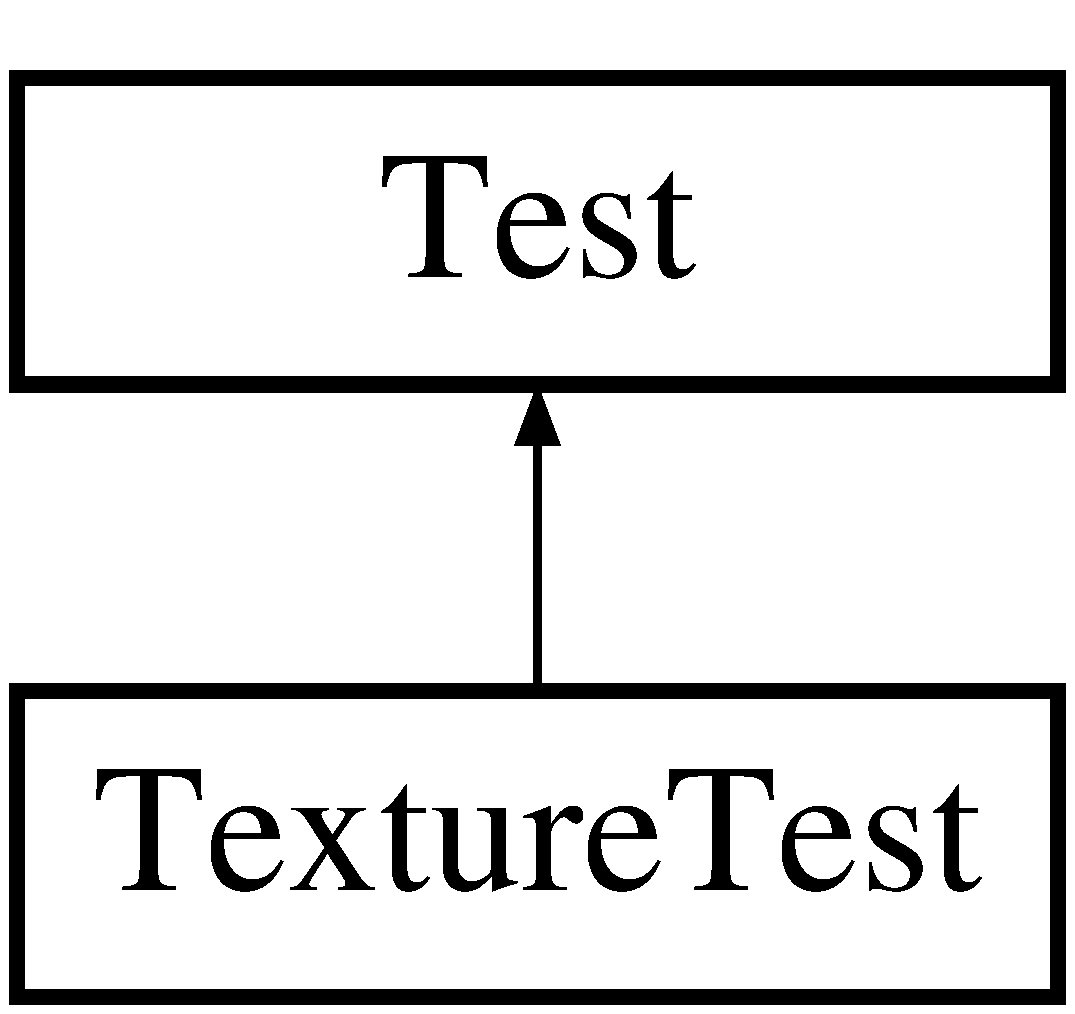
\includegraphics[height=2.000000cm]{classTextureTest}
\end{center}
\end{figure}
\subsection*{Public Member Functions}
\begin{DoxyCompactItemize}
\item 
\mbox{\Hypertarget{classTextureTest_a8cca7d9a0760cb391be5d9e6fb51f486}\label{classTextureTest_a8cca7d9a0760cb391be5d9e6fb51f486}} 
virtual void {\bfseries Set\+Up} ()
\item 
\mbox{\Hypertarget{classTextureTest_aaa60dee1e4561c37c49dd4736783e120}\label{classTextureTest_aaa60dee1e4561c37c49dd4736783e120}} 
virtual void {\bfseries Tear\+Down} ()
\end{DoxyCompactItemize}
\subsection*{Public Attributes}
\begin{DoxyCompactItemize}
\item 
\mbox{\Hypertarget{classTextureTest_a1b0d48fea35d6bdadae4e1856cf12e21}\label{classTextureTest_a1b0d48fea35d6bdadae4e1856cf12e21}} 
\hyperlink{classSDLMock}{S\+D\+L\+Mock} $\ast$ {\bfseries mock}
\end{DoxyCompactItemize}


\subsection{Detailed Description}


Definition at line 36 of file Texture\+Test.\+h.



The documentation for this class was generated from the following file\+:\begin{DoxyCompactItemize}
\item 
/home/skaupper/dev/\+B\+K\+Engine/tests/Texture\+Test.\+h\end{DoxyCompactItemize}

\hypertarget{classbkengine_1_1TextureWrapper}{}\section{bkengine\+:\+:Texture\+Wrapper Class Reference}
\label{classbkengine_1_1TextureWrapper}\index{bkengine\+::\+Texture\+Wrapper@{bkengine\+::\+Texture\+Wrapper}}
\subsection*{Public Member Functions}
\begin{DoxyCompactItemize}
\item 
\mbox{\Hypertarget{classbkengine_1_1TextureWrapper_aa33c372bc5b664f584884525ca0d09fa}\label{classbkengine_1_1TextureWrapper_aa33c372bc5b664f584884525ca0d09fa}} 
{\bfseries Texture\+Wrapper} (S\+D\+L\+\_\+\+Texture $\ast$tex, const std\+::string \&path)
\item 
\mbox{\Hypertarget{classbkengine_1_1TextureWrapper_a8c71398da302ff4fdb21c631f8ba7fbe}\label{classbkengine_1_1TextureWrapper_a8c71398da302ff4fdb21c631f8ba7fbe}} 
{\bfseries Texture\+Wrapper} (S\+D\+L\+\_\+\+Texture $\ast$tex, const std\+::string \&text, const std\+::string \&font\+Name, \hyperlink{structbkengine_1_1Color}{Color} c, Text\+Quality quality)
\item 
\mbox{\Hypertarget{classbkengine_1_1TextureWrapper_ab6682dd9e08515e7ae7cf9c6315952ab}\label{classbkengine_1_1TextureWrapper_ab6682dd9e08515e7ae7cf9c6315952ab}} 
S\+D\+L\+\_\+\+Texture $\ast$ {\bfseries get} () const
\item 
\mbox{\Hypertarget{classbkengine_1_1TextureWrapper_a92879535f9315c64449f075e8e9eb24d}\label{classbkengine_1_1TextureWrapper_a92879535f9315c64449f075e8e9eb24d}} 
void {\bfseries set} (S\+D\+L\+\_\+\+Texture $\ast$tex)
\item 
\mbox{\Hypertarget{classbkengine_1_1TextureWrapper_aaf2f6ae04d38d6f855753521ea299547}\label{classbkengine_1_1TextureWrapper_aaf2f6ae04d38d6f855753521ea299547}} 
void {\bfseries free} ()
\item 
\mbox{\Hypertarget{classbkengine_1_1TextureWrapper_aa349172b01bf01501c1454f8bb6f88a6}\label{classbkengine_1_1TextureWrapper_aa349172b01bf01501c1454f8bb6f88a6}} 
\hyperlink{structbkengine_1_1Rect}{Rect} {\bfseries get\+Size} () const
\end{DoxyCompactItemize}
\subsection*{Friends}
\begin{DoxyCompactItemize}
\item 
\mbox{\Hypertarget{classbkengine_1_1TextureWrapper_af7f909106d08e36cd50aa58e36f9bf47}\label{classbkengine_1_1TextureWrapper_af7f909106d08e36cd50aa58e36f9bf47}} 
class {\bfseries Texture}
\end{DoxyCompactItemize}


\subsection{Detailed Description}


Definition at line 98 of file Misc.\+h.



The documentation for this class was generated from the following files\+:\begin{DoxyCompactItemize}
\item 
/home/skaupper/dev/\+B\+K\+Engine/include/bkengine/Misc.\+h\item 
/home/skaupper/dev/\+B\+K\+Engine/src/Misc.\+cpp\end{DoxyCompactItemize}

\hypertarget{classbkengine_1_1Timer}{}\section{bkengine\+:\+:Timer Class Reference}
\label{classbkengine_1_1Timer}\index{bkengine\+::\+Timer@{bkengine\+::\+Timer}}
\subsection*{Public Member Functions}
\begin{DoxyCompactItemize}
\item 
\mbox{\Hypertarget{classbkengine_1_1Timer_a3a8b5272198d029779dc9302a54305a8}\label{classbkengine_1_1Timer_a3a8b5272198d029779dc9302a54305a8}} 
void {\bfseries start} ()
\item 
\mbox{\Hypertarget{classbkengine_1_1Timer_a63f0eb44b27402196590a03781515dba}\label{classbkengine_1_1Timer_a63f0eb44b27402196590a03781515dba}} 
void {\bfseries stop} ()
\item 
\mbox{\Hypertarget{classbkengine_1_1Timer_a0289effad7b573c508bc27e405900a23}\label{classbkengine_1_1Timer_a0289effad7b573c508bc27e405900a23}} 
void {\bfseries pause} ()
\item 
\mbox{\Hypertarget{classbkengine_1_1Timer_aa4dd50d7ed48ac73efed2950749d35d6}\label{classbkengine_1_1Timer_aa4dd50d7ed48ac73efed2950749d35d6}} 
void {\bfseries unpause} ()
\item 
\mbox{\Hypertarget{classbkengine_1_1Timer_a867fa6b90d7e3e0595e1469450b95210}\label{classbkengine_1_1Timer_a867fa6b90d7e3e0595e1469450b95210}} 
int {\bfseries get\+Ticks} () const
\item 
\mbox{\Hypertarget{classbkengine_1_1Timer_ac52c3294294bd363fa029bf382dab204}\label{classbkengine_1_1Timer_ac52c3294294bd363fa029bf382dab204}} 
bool {\bfseries is\+Started} () const
\item 
\mbox{\Hypertarget{classbkengine_1_1Timer_ad5a769d16483dde076721b30bfdbeb73}\label{classbkengine_1_1Timer_ad5a769d16483dde076721b30bfdbeb73}} 
bool {\bfseries is\+Paused} () const
\end{DoxyCompactItemize}


\subsection{Detailed Description}


Definition at line 8 of file Timer.\+h.



The documentation for this class was generated from the following files\+:\begin{DoxyCompactItemize}
\item 
/home/skaupper/dev/\+B\+K\+Engine/include/bkengine/Timer.\+h\item 
/home/skaupper/dev/\+B\+K\+Engine/src/Timer.\+cpp\end{DoxyCompactItemize}

\hypertarget{structbkengine_1_1WheelEvent}{}\section{bkengine\+:\+:Wheel\+Event Struct Reference}
\label{structbkengine_1_1WheelEvent}\index{bkengine\+::\+Wheel\+Event@{bkengine\+::\+Wheel\+Event}}
\subsection*{Public Attributes}
\begin{DoxyCompactItemize}
\item 
\mbox{\Hypertarget{structbkengine_1_1WheelEvent_a8dff42b278014781dcfea71e45fc10e8}\label{structbkengine_1_1WheelEvent_a8dff42b278014781dcfea71e45fc10e8}} 
int32\+\_\+t {\bfseries x}
\item 
\mbox{\Hypertarget{structbkengine_1_1WheelEvent_ad4cecaa9119eef57325a503ce0746eff}\label{structbkengine_1_1WheelEvent_ad4cecaa9119eef57325a503ce0746eff}} 
int32\+\_\+t {\bfseries y}
\item 
\mbox{\Hypertarget{structbkengine_1_1WheelEvent_adafbc85c70ddf5cc485c2dd1228d8801}\label{structbkengine_1_1WheelEvent_adafbc85c70ddf5cc485c2dd1228d8801}} 
Wheel\+Direction {\bfseries direction}
\end{DoxyCompactItemize}


\subsection{Detailed Description}


Definition at line 76 of file Event.\+h.



The documentation for this struct was generated from the following file\+:\begin{DoxyCompactItemize}
\item 
/home/skaupper/dev/\+B\+K\+Engine/include/bkengine/Event.\+h\end{DoxyCompactItemize}

\hypertarget{structbkengine_1_1WindowEvent}{}\section{bkengine\+:\+:Window\+Event Struct Reference}
\label{structbkengine_1_1WindowEvent}\index{bkengine\+::\+Window\+Event@{bkengine\+::\+Window\+Event}}
\subsection*{Public Attributes}
\begin{DoxyCompactItemize}
\item 
\mbox{\Hypertarget{structbkengine_1_1WindowEvent_ad03317d9c4222438ba3e9321fa0f2f9a}\label{structbkengine_1_1WindowEvent_ad03317d9c4222438ba3e9321fa0f2f9a}} 
Window\+Event\+Type {\bfseries type}
\item 
\mbox{\Hypertarget{structbkengine_1_1WindowEvent_a1dc5d858cd7ecd44bed9810e41544b85}\label{structbkengine_1_1WindowEvent_a1dc5d858cd7ecd44bed9810e41544b85}} 
std\+::vector$<$ int32\+\_\+t $>$ {\bfseries data}
\end{DoxyCompactItemize}


\subsection{Detailed Description}


Definition at line 82 of file Event.\+h.



The documentation for this struct was generated from the following file\+:\begin{DoxyCompactItemize}
\item 
/home/skaupper/dev/\+B\+K\+Engine/include/bkengine/Event.\+h\end{DoxyCompactItemize}

%--- End generated contents ---

% Index
\backmatter
\newpage
\phantomsection
\clearemptydoublepage
\addcontentsline{toc}{chapter}{Index}
\printindex

\end{document}
